\documentclass[twoside]{book}

% Packages required by doxygen
\usepackage{fixltx2e}
\usepackage{calc}
\usepackage{doxygen}
\usepackage[export]{adjustbox} % also loads graphicx
\usepackage{graphicx}
\usepackage[utf8]{inputenc}
\usepackage{makeidx}
\usepackage{multicol}
\usepackage{multirow}
\PassOptionsToPackage{warn}{textcomp}
\usepackage{textcomp}
\usepackage[nointegrals]{wasysym}
\usepackage[table]{xcolor}

% Font selection
\usepackage[T1]{fontenc}
\usepackage[scaled=.90]{helvet}
\usepackage{courier}
\usepackage{amssymb}
\usepackage{sectsty}
\renewcommand{\familydefault}{\sfdefault}
\allsectionsfont{%
  \fontseries{bc}\selectfont%
  \color{darkgray}%
}
\renewcommand{\DoxyLabelFont}{%
  \fontseries{bc}\selectfont%
  \color{darkgray}%
}
\newcommand{\+}{\discretionary{\mbox{\scriptsize$\hookleftarrow$}}{}{}}

% Page & text layout
\usepackage{geometry}
\geometry{%
  a4paper,%
  top=2.5cm,%
  bottom=2.5cm,%
  left=2.5cm,%
  right=2.5cm%
}
\tolerance=750
\hfuzz=15pt
\hbadness=750
\setlength{\emergencystretch}{15pt}
\setlength{\parindent}{0cm}
\setlength{\parskip}{3ex plus 2ex minus 2ex}
\makeatletter
\renewcommand{\paragraph}{%
  \@startsection{paragraph}{4}{0ex}{-1.0ex}{1.0ex}{%
    \normalfont\normalsize\bfseries\SS@parafont%
  }%
}
\renewcommand{\subparagraph}{%
  \@startsection{subparagraph}{5}{0ex}{-1.0ex}{1.0ex}{%
    \normalfont\normalsize\bfseries\SS@subparafont%
  }%
}
\makeatother

% Headers & footers
\usepackage{fancyhdr}
\pagestyle{fancyplain}
\fancyhead[LE]{\fancyplain{}{\bfseries\thepage}}
\fancyhead[CE]{\fancyplain{}{}}
\fancyhead[RE]{\fancyplain{}{\bfseries\leftmark}}
\fancyhead[LO]{\fancyplain{}{\bfseries\rightmark}}
\fancyhead[CO]{\fancyplain{}{}}
\fancyhead[RO]{\fancyplain{}{\bfseries\thepage}}
\fancyfoot[LE]{\fancyplain{}{}}
\fancyfoot[CE]{\fancyplain{}{}}
\fancyfoot[RE]{\fancyplain{}{\bfseries\scriptsize Generated by Doxygen }}
\fancyfoot[LO]{\fancyplain{}{\bfseries\scriptsize Generated by Doxygen }}
\fancyfoot[CO]{\fancyplain{}{}}
\fancyfoot[RO]{\fancyplain{}{}}
\renewcommand{\footrulewidth}{0.4pt}
\renewcommand{\chaptermark}[1]{%
  \markboth{#1}{}%
}
\renewcommand{\sectionmark}[1]{%
  \markright{\thesection\ #1}%
}

% Indices & bibliography
\usepackage{natbib}
\usepackage[titles]{tocloft}
\setcounter{tocdepth}{3}
\setcounter{secnumdepth}{5}
\makeindex

% Hyperlinks (required, but should be loaded last)
\usepackage{ifpdf}
\ifpdf
  \usepackage[pdftex,pagebackref=true]{hyperref}
\else
  \usepackage[ps2pdf,pagebackref=true]{hyperref}
\fi
\hypersetup{%
  colorlinks=true,%
  linkcolor=blue,%
  citecolor=blue,%
  unicode%
}

% Custom commands
\newcommand{\clearemptydoublepage}{%
  \newpage{\pagestyle{empty}\cleardoublepage}%
}

\usepackage{caption}
\captionsetup{labelsep=space,justification=centering,font={bf},singlelinecheck=off,skip=4pt,position=top}

%===== C O N T E N T S =====

\begin{document}

% Titlepage & ToC
\hypersetup{pageanchor=false,
             bookmarksnumbered=true,
             pdfencoding=unicode
            }
\pagenumbering{alph}
\begin{titlepage}
\vspace*{7cm}
\begin{center}%
{\Large Wild\+Life Tracker Services }\\
\vspace*{1cm}
{\large Generated by Doxygen 1.8.13}\\
\end{center}
\end{titlepage}
\clearemptydoublepage
\pagenumbering{roman}
\tableofcontents
\clearemptydoublepage
\pagenumbering{arabic}
\hypersetup{pageanchor=true}

%--- Begin generated contents ---
\chapter{Namespace Index}
\section{Namespace List}
Here is a list of all namespaces with brief descriptions\+:\begin{DoxyCompactList}
\item\contentsline{section}{\hyperlink{namespaceWildlifeTrackingApp}{Wildlife\+Tracking\+App} }{\pageref{namespaceWildlifeTrackingApp}}{}
\item\contentsline{section}{\hyperlink{namespaceWildlifeTrackingApp_1_1Delegates}{Wildlife\+Tracking\+App.\+Delegates} }{\pageref{namespaceWildlifeTrackingApp_1_1Delegates}}{}
\item\contentsline{section}{\hyperlink{namespaceWildlifeTrackingApp_1_1Models}{Wildlife\+Tracking\+App.\+Models} }{\pageref{namespaceWildlifeTrackingApp_1_1Models}}{}
\item\contentsline{section}{\hyperlink{namespaceWildlifeTrackingApp_1_1Properties}{Wildlife\+Tracking\+App.\+Properties} }{\pageref{namespaceWildlifeTrackingApp_1_1Properties}}{}
\item\contentsline{section}{\hyperlink{namespaceWildlifeTrackingApp_1_1Utility}{Wildlife\+Tracking\+App.\+Utility} }{\pageref{namespaceWildlifeTrackingApp_1_1Utility}}{}
\end{DoxyCompactList}

\chapter{Hierarchical Index}
\section{Class Hierarchy}
This inheritance list is sorted roughly, but not completely, alphabetically\+:\begin{DoxyCompactList}
\item Form\begin{DoxyCompactList}
\item \contentsline{section}{Add\+\_\+\+G\+PS}{\pageref{classWildlifeTrackingApp_1_1Add__GPS}}{}
\item \contentsline{section}{Add\+Category}{\pageref{classWildlifeTrackingApp_1_1AddCategory}}{}
\item \contentsline{section}{Animal\+Name}{\pageref{classWildlifeTrackingApp_1_1AnimalName}}{}
\item \contentsline{section}{Category}{\pageref{classWildlifeTrackingApp_1_1Category}}{}
\item \contentsline{section}{G\+P\+S\+Device}{\pageref{classWildlifeTrackingApp_1_1GPSDevice}}{}
\item \contentsline{section}{Locate\+Category}{\pageref{classWildlifeTrackingApp_1_1LocateCategory}}{}
\item \contentsline{section}{Main\+Page}{\pageref{classWildlifeTrackingApp_1_1MainPage}}{}
\item \contentsline{section}{Pop\+Up}{\pageref{classWildlifeTrackingApp_1_1PopUp}}{}
\item \contentsline{section}{Report}{\pageref{classWildlifeTrackingApp_1_1Report}}{}
\end{DoxyCompactList}
\item Application\+Settings\+Base\begin{DoxyCompactList}
\item \contentsline{section}{Settings}{\pageref{classWildlifeTrackingApp_1_1Properties_1_1Settings}}{}
\end{DoxyCompactList}
\item \contentsline{section}{Animal\+Delegate}{\pageref{classWildlifeTrackingApp_1_1Delegates_1_1AnimalDelegate}}{}
\item \contentsline{section}{Category\+Delegate}{\pageref{classWildlifeTrackingApp_1_1Delegates_1_1CategoryDelegate}}{}
\item \contentsline{section}{Tracking\+Info\+Delegate}{\pageref{classWildlifeTrackingApp_1_1Delegates_1_1TrackingInfoDelegate}}{}
\item \contentsline{section}{Animal}{\pageref{classWildlifeTrackingApp_1_1Models_1_1Animal}}{}
\item \contentsline{section}{Animal\+Category\+Count}{\pageref{classWildlifeTrackingApp_1_1Models_1_1AnimalCategoryCount}}{}
\item \contentsline{section}{Animal\+Response\+View}{\pageref{classWildlifeTrackingApp_1_1Models_1_1AnimalResponseView}}{}
\item \contentsline{section}{Category\+Response\+View}{\pageref{classWildlifeTrackingApp_1_1Models_1_1CategoryResponseView}}{}
\item \contentsline{section}{Response}{\pageref{classWildlifeTrackingApp_1_1Models_1_1Response}}{}
\begin{DoxyCompactList}
\item \contentsline{section}{Category}{\pageref{classWildlifeTrackingApp_1_1Models_1_1Category}}{}
\end{DoxyCompactList}
\item \contentsline{section}{Tracking\+Info}{\pageref{classWildlifeTrackingApp_1_1Models_1_1TrackingInfo}}{}
\item \contentsline{section}{Tracking\+Response\+View}{\pageref{classWildlifeTrackingApp_1_1Models_1_1TrackingResponseView}}{}
\item \contentsline{section}{Program}{\pageref{classWildlifeTrackingApp_1_1Program}}{}
\item \contentsline{section}{Resources}{\pageref{classWildlifeTrackingApp_1_1Properties_1_1Resources}}{}
\item \contentsline{section}{Constants}{\pageref{classWildlifeTrackingApp_1_1Utility_1_1Constants}}{}
\item \contentsline{section}{Http\+Util}{\pageref{classWildlifeTrackingApp_1_1Utility_1_1HttpUtil}}{}
\end{DoxyCompactList}

\chapter{Class Index}
\section{Class List}
Here are the classes, structs, unions and interfaces with brief descriptions\+:\begin{DoxyCompactList}
\item\contentsline{section}{\hyperlink{classWildLifeTracker_1_1CategoryService}{Category\+Service} \\*Category Service to perform different operations. }{\pageref{classWildLifeTracker_1_1CategoryService}}{}
\item\contentsline{section}{\hyperlink{classWildLifeTracker_1_1game__reserve__dbEntities}{game\+\_\+reserve\+\_\+db\+Entities} }{\pageref{classWildLifeTracker_1_1game__reserve__dbEntities}}{}
\item\contentsline{section}{\hyperlink{interfaceWildLifeTracker_1_1ICategoryService}{I\+Category\+Service} \\*The interface exposes all the A\+P\+Is for category details }{\pageref{interfaceWildLifeTracker_1_1ICategoryService}}{}
\item\contentsline{section}{\hyperlink{classWildLifeTracker_1_1Models_1_1Animal}{Animal} }{\pageref{classWildLifeTracker_1_1Models_1_1Animal}}{}
\item\contentsline{section}{\hyperlink{classWildLifeTracker_1_1Models_1_1AnimalCount}{Animal\+Count} }{\pageref{classWildLifeTracker_1_1Models_1_1AnimalCount}}{}
\item\contentsline{section}{\hyperlink{classWildLifeTracker_1_1Models_1_1Category}{Category} }{\pageref{classWildLifeTracker_1_1Models_1_1Category}}{}
\item\contentsline{section}{\hyperlink{classWildLifeTracker_1_1Models_1_1GPSTrackingInfo}{G\+P\+S\+Tracking\+Info} }{\pageref{classWildLifeTracker_1_1Models_1_1GPSTrackingInfo}}{}
\item\contentsline{section}{\hyperlink{classWildLifeTracker_1_1Repository_1_1AnimalRepo}{Animal\+Repo} \\*The class is used to fetch the animals details from DB or save it in the DB }{\pageref{classWildLifeTracker_1_1Repository_1_1AnimalRepo}}{}
\item\contentsline{section}{\hyperlink{classWildLifeTracker_1_1Repository_1_1CategoryRepo}{Category\+Repo} \\*This class is used to add, update, delete and retrieve the category details. }{\pageref{classWildLifeTracker_1_1Repository_1_1CategoryRepo}}{}
\item\contentsline{section}{\hyperlink{classWildLifeTracker_1_1Repository_1_1TrackingRepo}{Tracking\+Repo} \\*The class is used to store the G\+PS Location and retrieve the latest position of animals }{\pageref{classWildLifeTracker_1_1Repository_1_1TrackingRepo}}{}
\item\contentsline{section}{\hyperlink{classWildLifeTracker_1_1Response_1_1AnimalResponse}{Animal\+Response} \\*The model is used to create a response for animal operation }{\pageref{classWildLifeTracker_1_1Response_1_1AnimalResponse}}{}
\item\contentsline{section}{\hyperlink{classWildLifeTracker_1_1Response_1_1CategoryResponse}{Category\+Response} \\*The model is used to create a response for category operation }{\pageref{classWildLifeTracker_1_1Response_1_1CategoryResponse}}{}
\item\contentsline{section}{\hyperlink{classWildLifeTracker_1_1Response_1_1Response}{Response} }{\pageref{classWildLifeTracker_1_1Response_1_1Response}}{}
\item\contentsline{section}{\hyperlink{classWildLifeTracker_1_1Response_1_1TrackingInfoResponse}{Tracking\+Info\+Response} \\*The model is used to create a response for tracking operation }{\pageref{classWildLifeTracker_1_1Response_1_1TrackingInfoResponse}}{}
\item\contentsline{section}{\hyperlink{classWildLifeTracker_1_1Services_1_1AnimalService}{Animal\+Service} \\*Animal Service to perform different operations. }{\pageref{classWildLifeTracker_1_1Services_1_1AnimalService}}{}
\item\contentsline{section}{\hyperlink{interfaceWildLifeTracker_1_1Services_1_1IAnimalService}{I\+Animal\+Service} \\*The interface exposes all the A\+P\+Is for animal details }{\pageref{interfaceWildLifeTracker_1_1Services_1_1IAnimalService}}{}
\item\contentsline{section}{\hyperlink{interfaceWildLifeTracker_1_1Services_1_1ITrackingInfoService}{I\+Tracking\+Info\+Service} \\*The interface exposes all the A\+P\+Is for tracking details }{\pageref{interfaceWildLifeTracker_1_1Services_1_1ITrackingInfoService}}{}
\item\contentsline{section}{\hyperlink{classWildLifeTracker_1_1Services_1_1TrackingInfoService}{Tracking\+Info\+Service} \\*Tracking Service to perform different operations. }{\pageref{classWildLifeTracker_1_1Services_1_1TrackingInfoService}}{}
\item\contentsline{section}{\hyperlink{classWildLifeTracker_1_1tblanimal}{tblanimal} }{\pageref{classWildLifeTracker_1_1tblanimal}}{}
\item\contentsline{section}{\hyperlink{classWildLifeTracker_1_1tblcategory}{tblcategory} }{\pageref{classWildLifeTracker_1_1tblcategory}}{}
\item\contentsline{section}{\hyperlink{classWildLifeTracker_1_1tblgpstracking}{tblgpstracking} }{\pageref{classWildLifeTracker_1_1tblgpstracking}}{}
\item\contentsline{section}{\hyperlink{classWildLifeTracker_1_1Utility_1_1ErrorHandler}{Error\+Handler} }{\pageref{classWildLifeTracker_1_1Utility_1_1ErrorHandler}}{}
\end{DoxyCompactList}

\chapter{File Index}
\section{File List}
Here is a list of all files with brief descriptions\+:\begin{DoxyCompactList}
\item\contentsline{section}{\hyperlink{AnimalName_8cs}{Animal\+Name.\+cs} }{\pageref{AnimalName_8cs}}{}
\item\contentsline{section}{\hyperlink{AnimalName_8Designer_8cs}{Animal\+Name.\+Designer.\+cs} }{\pageref{AnimalName_8Designer_8cs}}{}
\item\contentsline{section}{\hyperlink{Program_8cs}{Program.\+cs} }{\pageref{Program_8cs}}{}
\item\contentsline{section}{Delegates/\hyperlink{AnimalDelegate_8cs}{Animal\+Delegate.\+cs} }{\pageref{AnimalDelegate_8cs}}{}
\item\contentsline{section}{Delegates/\hyperlink{CategoryDelegate_8cs}{Category\+Delegate.\+cs} }{\pageref{CategoryDelegate_8cs}}{}
\item\contentsline{section}{Delegates/\hyperlink{TrackingInfoDelegate_8cs}{Tracking\+Info\+Delegate.\+cs} }{\pageref{TrackingInfoDelegate_8cs}}{}
\item\contentsline{section}{Models/\hyperlink{Animal_8cs}{Animal.\+cs} }{\pageref{Animal_8cs}}{}
\item\contentsline{section}{Models/\hyperlink{AnimalCategoryCount_8cs}{Animal\+Category\+Count.\+cs} }{\pageref{AnimalCategoryCount_8cs}}{}
\item\contentsline{section}{Models/\hyperlink{AnimalResponseView_8cs}{Animal\+Response\+View.\+cs} }{\pageref{AnimalResponseView_8cs}}{}
\item\contentsline{section}{Models/\hyperlink{Models_2Category_8cs}{Category.\+cs} }{\pageref{Models_2Category_8cs}}{}
\item\contentsline{section}{Models/\hyperlink{CategoryResponseView_8cs}{Category\+Response\+View.\+cs} }{\pageref{CategoryResponseView_8cs}}{}
\item\contentsline{section}{Models/\hyperlink{Response_8cs}{Response.\+cs} }{\pageref{Response_8cs}}{}
\item\contentsline{section}{Models/\hyperlink{TrackingInfo_8cs}{Tracking\+Info.\+cs} }{\pageref{TrackingInfo_8cs}}{}
\item\contentsline{section}{Models/\hyperlink{TrackingResponseView_8cs}{Tracking\+Response\+View.\+cs} }{\pageref{TrackingResponseView_8cs}}{}
\item\contentsline{section}{obj/\+Debug/\hyperlink{TemporaryGeneratedFile__036C0B5B-1481-4323-8D20-8F5ADCB23D92_8cs}{Temporary\+Generated\+File\+\_\+036\+C0\+B5\+B-\/1481-\/4323-\/8\+D20-\/8\+F5\+A\+D\+C\+B23\+D92.\+cs} }{\pageref{TemporaryGeneratedFile__036C0B5B-1481-4323-8D20-8F5ADCB23D92_8cs}}{}
\item\contentsline{section}{obj/\+Debug/\hyperlink{TemporaryGeneratedFile__5937a670-0e60-4077-877b-f7221da3dda1_8cs}{Temporary\+Generated\+File\+\_\+5937a670-\/0e60-\/4077-\/877b-\/f7221da3dda1.\+cs} }{\pageref{TemporaryGeneratedFile__5937a670-0e60-4077-877b-f7221da3dda1_8cs}}{}
\item\contentsline{section}{obj/\+Debug/\hyperlink{TemporaryGeneratedFile__E7A71F73-0F8D-4B9B-B56E-8E70B10BC5D3_8cs}{Temporary\+Generated\+File\+\_\+\+E7\+A71\+F73-\/0\+F8\+D-\/4\+B9\+B-\/\+B56\+E-\/8\+E70\+B10\+B\+C5\+D3.\+cs} }{\pageref{TemporaryGeneratedFile__E7A71F73-0F8D-4B9B-B56E-8E70B10BC5D3_8cs}}{}
\item\contentsline{section}{Properties/\hyperlink{AssemblyInfo_8cs}{Assembly\+Info.\+cs} }{\pageref{AssemblyInfo_8cs}}{}
\item\contentsline{section}{Properties/\hyperlink{Resources_8Designer_8cs}{Resources.\+Designer.\+cs} }{\pageref{Resources_8Designer_8cs}}{}
\item\contentsline{section}{Properties/\hyperlink{Settings_8Designer_8cs}{Settings.\+Designer.\+cs} }{\pageref{Settings_8Designer_8cs}}{}
\item\contentsline{section}{Resources/\hyperlink{do-sharp_8php}{do-\/sharp.\+php} }{\pageref{do-sharp_8php}}{}
\item\contentsline{section}{Resources/\hyperlink{do-sharp1_8php}{do-\/sharp1.\+php} }{\pageref{do-sharp1_8php}}{}
\item\contentsline{section}{Utility/\hyperlink{Constants_8cs}{Constants.\+cs} }{\pageref{Constants_8cs}}{}
\item\contentsline{section}{Utility/\hyperlink{HttpUtil_8cs}{Http\+Util.\+cs} }{\pageref{HttpUtil_8cs}}{}
\item\contentsline{section}{View/\hyperlink{Add_01GPS_8cs}{Add G\+P\+S.\+cs} }{\pageref{Add_01GPS_8cs}}{}
\item\contentsline{section}{View/\hyperlink{Add_01GPS_8Designer_8cs}{Add G\+P\+S.\+Designer.\+cs} }{\pageref{Add_01GPS_8Designer_8cs}}{}
\item\contentsline{section}{View/\hyperlink{AddCategory_8cs}{Add\+Category.\+cs} }{\pageref{AddCategory_8cs}}{}
\item\contentsline{section}{View/\hyperlink{AddCategory_8Designer_8cs}{Add\+Category.\+Designer.\+cs} }{\pageref{AddCategory_8Designer_8cs}}{}
\item\contentsline{section}{View/\hyperlink{View_2Category_8cs}{Category.\+cs} }{\pageref{View_2Category_8cs}}{}
\item\contentsline{section}{View/\hyperlink{Category_8Designer_8cs}{Category.\+Designer.\+cs} }{\pageref{Category_8Designer_8cs}}{}
\item\contentsline{section}{View/\hyperlink{GPSDevice_8cs}{G\+P\+S\+Device.\+cs} }{\pageref{GPSDevice_8cs}}{}
\item\contentsline{section}{View/\hyperlink{GPSDevice_8Designer_8cs}{G\+P\+S\+Device.\+Designer.\+cs} }{\pageref{GPSDevice_8Designer_8cs}}{}
\item\contentsline{section}{View/\hyperlink{LocateCategory_8cs}{Locate\+Category.\+cs} }{\pageref{LocateCategory_8cs}}{}
\item\contentsline{section}{View/\hyperlink{LocateCategory_8Designer_8cs}{Locate\+Category.\+Designer.\+cs} }{\pageref{LocateCategory_8Designer_8cs}}{}
\item\contentsline{section}{View/\hyperlink{MainPage_8cs}{Main\+Page.\+cs} }{\pageref{MainPage_8cs}}{}
\item\contentsline{section}{View/\hyperlink{MainPage_8Designer_8cs}{Main\+Page.\+Designer.\+cs} }{\pageref{MainPage_8Designer_8cs}}{}
\item\contentsline{section}{View/\hyperlink{PopUp_8cs}{Pop\+Up.\+cs} }{\pageref{PopUp_8cs}}{}
\item\contentsline{section}{View/\hyperlink{PopUp_8Designer_8cs}{Pop\+Up.\+Designer.\+cs} }{\pageref{PopUp_8Designer_8cs}}{}
\item\contentsline{section}{View/\hyperlink{Report_8cs}{Report.\+cs} }{\pageref{Report_8cs}}{}
\item\contentsline{section}{View/\hyperlink{Report_8Designer_8cs}{Report.\+Designer.\+cs} }{\pageref{Report_8Designer_8cs}}{}
\end{DoxyCompactList}

\chapter{Namespace Documentation}
\hypertarget{namespaceWildLifeTracker}{}\section{Wild\+Life\+Tracker Namespace Reference}
\label{namespaceWildLifeTracker}\index{Wild\+Life\+Tracker@{Wild\+Life\+Tracker}}
\subsection*{Namespaces}
\begin{DoxyCompactItemize}
\item 
namespace \hyperlink{namespaceWildLifeTracker_1_1Models}{Models}
\item 
namespace \hyperlink{namespaceWildLifeTracker_1_1Repository}{Repository}
\item 
namespace \hyperlink{namespaceWildLifeTracker_1_1Response}{Response}
\item 
namespace \hyperlink{namespaceWildLifeTracker_1_1Services}{Services}
\item 
namespace \hyperlink{namespaceWildLifeTracker_1_1Utility}{Utility}
\end{DoxyCompactItemize}
\subsection*{Classes}
\begin{DoxyCompactItemize}
\item 
class \hyperlink{classWildLifeTracker_1_1CategoryService}{Category\+Service}
\begin{DoxyCompactList}\small\item\em Category Service to perform different operations. \end{DoxyCompactList}\item 
class \hyperlink{classWildLifeTracker_1_1game__reserve__dbEntities}{game\+\_\+reserve\+\_\+db\+Entities}
\item 
interface \hyperlink{interfaceWildLifeTracker_1_1ICategoryService}{I\+Category\+Service}
\begin{DoxyCompactList}\small\item\em The interface exposes all the A\+P\+Is for category details \end{DoxyCompactList}\item 
class \hyperlink{classWildLifeTracker_1_1tblanimal}{tblanimal}
\item 
class \hyperlink{classWildLifeTracker_1_1tblcategory}{tblcategory}
\item 
class \hyperlink{classWildLifeTracker_1_1tblgpstracking}{tblgpstracking}
\end{DoxyCompactItemize}

\hypertarget{namespaceWildLifeTracker_1_1Models}{}\section{Wild\+Life\+Tracker.\+Models Namespace Reference}
\label{namespaceWildLifeTracker_1_1Models}\index{Wild\+Life\+Tracker.\+Models@{Wild\+Life\+Tracker.\+Models}}
\subsection*{Classes}
\begin{DoxyCompactItemize}
\item 
class \hyperlink{classWildLifeTracker_1_1Models_1_1Animal}{Animal}
\item 
class \hyperlink{classWildLifeTracker_1_1Models_1_1AnimalCount}{Animal\+Count}
\item 
class \hyperlink{classWildLifeTracker_1_1Models_1_1Category}{Category}
\item 
class \hyperlink{classWildLifeTracker_1_1Models_1_1GPSTrackingInfo}{G\+P\+S\+Tracking\+Info}
\end{DoxyCompactItemize}

\hypertarget{namespaceWildLifeTracker_1_1Repository}{}\section{Wild\+Life\+Tracker.\+Repository Namespace Reference}
\label{namespaceWildLifeTracker_1_1Repository}\index{Wild\+Life\+Tracker.\+Repository@{Wild\+Life\+Tracker.\+Repository}}
\subsection*{Classes}
\begin{DoxyCompactItemize}
\item 
class \hyperlink{classWildLifeTracker_1_1Repository_1_1AnimalRepo}{Animal\+Repo}
\begin{DoxyCompactList}\small\item\em The class is used to fetch the animals details from DB or save it in the DB \end{DoxyCompactList}\item 
class \hyperlink{classWildLifeTracker_1_1Repository_1_1CategoryRepo}{Category\+Repo}
\begin{DoxyCompactList}\small\item\em This class is used to add, update, delete and retrieve the category details. \end{DoxyCompactList}\item 
class \hyperlink{classWildLifeTracker_1_1Repository_1_1TrackingRepo}{Tracking\+Repo}
\begin{DoxyCompactList}\small\item\em The class is used to store the G\+PS Location and retrieve the latest position of animals \end{DoxyCompactList}\end{DoxyCompactItemize}

\hypertarget{namespaceWildLifeTracker_1_1Response}{}\section{Wild\+Life\+Tracker.\+Response Namespace Reference}
\label{namespaceWildLifeTracker_1_1Response}\index{Wild\+Life\+Tracker.\+Response@{Wild\+Life\+Tracker.\+Response}}
\subsection*{Classes}
\begin{DoxyCompactItemize}
\item 
class \hyperlink{classWildLifeTracker_1_1Response_1_1AnimalResponse}{Animal\+Response}
\begin{DoxyCompactList}\small\item\em The model is used to create a response for animal operation \end{DoxyCompactList}\item 
class \hyperlink{classWildLifeTracker_1_1Response_1_1CategoryResponse}{Category\+Response}
\begin{DoxyCompactList}\small\item\em The model is used to create a response for category operation \end{DoxyCompactList}\item 
class \hyperlink{classWildLifeTracker_1_1Response_1_1Response}{Response}
\item 
class \hyperlink{classWildLifeTracker_1_1Response_1_1TrackingInfoResponse}{Tracking\+Info\+Response}
\begin{DoxyCompactList}\small\item\em The model is used to create a response for tracking operation \end{DoxyCompactList}\end{DoxyCompactItemize}

\hypertarget{namespaceWildLifeTracker_1_1Services}{}\section{Wild\+Life\+Tracker.\+Services Namespace Reference}
\label{namespaceWildLifeTracker_1_1Services}\index{Wild\+Life\+Tracker.\+Services@{Wild\+Life\+Tracker.\+Services}}
\subsection*{Classes}
\begin{DoxyCompactItemize}
\item 
class \hyperlink{classWildLifeTracker_1_1Services_1_1AnimalService}{Animal\+Service}
\begin{DoxyCompactList}\small\item\em Animal Service to perform different operations. \end{DoxyCompactList}\item 
interface \hyperlink{interfaceWildLifeTracker_1_1Services_1_1IAnimalService}{I\+Animal\+Service}
\begin{DoxyCompactList}\small\item\em The interface exposes all the A\+P\+Is for animal details \end{DoxyCompactList}\item 
interface \hyperlink{interfaceWildLifeTracker_1_1Services_1_1ITrackingInfoService}{I\+Tracking\+Info\+Service}
\begin{DoxyCompactList}\small\item\em The interface exposes all the A\+P\+Is for tracking details \end{DoxyCompactList}\item 
class \hyperlink{classWildLifeTracker_1_1Services_1_1TrackingInfoService}{Tracking\+Info\+Service}
\begin{DoxyCompactList}\small\item\em Tracking Service to perform different operations. \end{DoxyCompactList}\end{DoxyCompactItemize}

\hypertarget{namespaceWildLifeTracker_1_1Utility}{}\section{Wild\+Life\+Tracker.\+Utility Namespace Reference}
\label{namespaceWildLifeTracker_1_1Utility}\index{Wild\+Life\+Tracker.\+Utility@{Wild\+Life\+Tracker.\+Utility}}
\subsection*{Classes}
\begin{DoxyCompactItemize}
\item 
class \hyperlink{classWildLifeTracker_1_1Utility_1_1ErrorHandler}{Error\+Handler}
\end{DoxyCompactItemize}

\chapter{Class Documentation}
\hypertarget{classWildLifeTracker_1_1CategoryService}{}\section{Category\+Service}
\label{classWildLifeTracker_1_1CategoryService}\index{Category\+Service@{Category\+Service}}


Category Service to perform different operations.  


Inheritance diagram for Category\+Service\+:\begin{figure}[H]
\begin{center}
\leavevmode
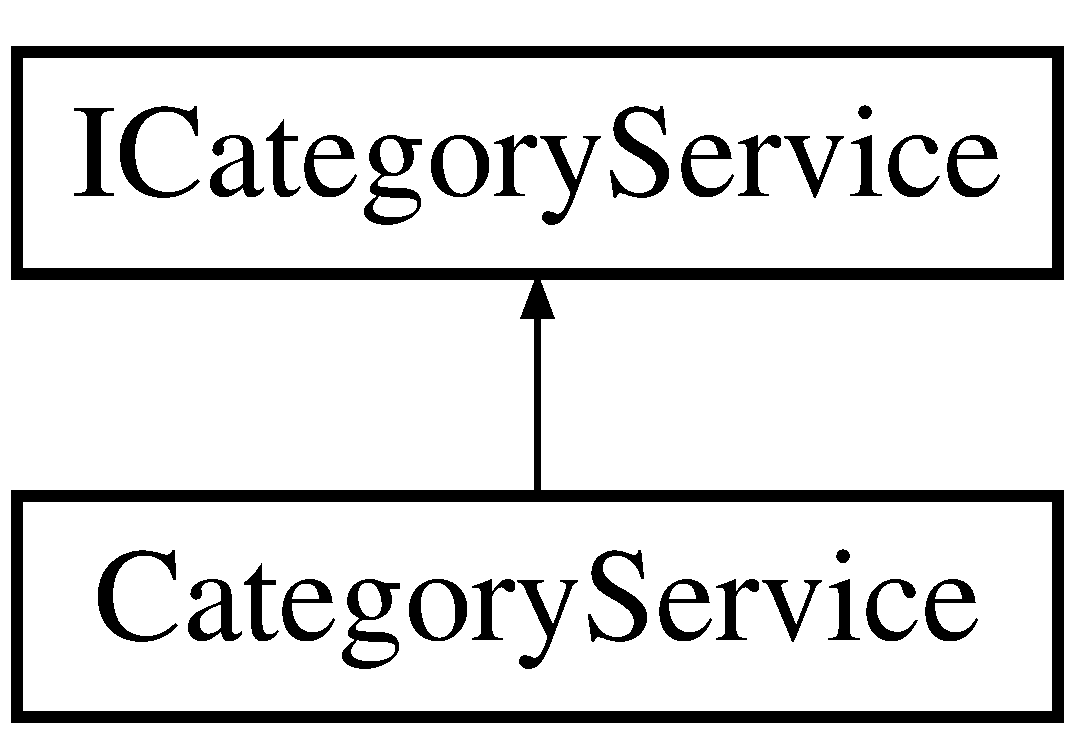
\includegraphics[height=2.000000cm]{classWildLifeTracker_1_1CategoryService}
\end{center}
\end{figure}
\subsection*{Public Member Functions}
\begin{DoxyCompactItemize}
\item 
\hyperlink{classWildLifeTracker_1_1CategoryService_a722357258ec21820efef6f642906457c}{Category\+Service} ()
\begin{DoxyCompactList}\small\item\em Constructor that intialize log4net in class \end{DoxyCompactList}\item 
\hyperlink{classWildLifeTracker_1_1Response_1_1CategoryResponse}{Category\+Response} \hyperlink{classWildLifeTracker_1_1CategoryService_ab22f6cdfb39adc2607dc86cb100889fc}{Add\+Category} (\hyperlink{classWildLifeTracker_1_1Models_1_1Category}{Category} category\+Details)
\begin{DoxyCompactList}\small\item\em Add a new category \end{DoxyCompactList}\item 
\hyperlink{classWildLifeTracker_1_1Response_1_1CategoryResponse}{Category\+Response} \hyperlink{classWildLifeTracker_1_1CategoryService_a6479e2a6945b14d40e8c57642e9d2665}{Delete\+Category} (string category\+Id)
\begin{DoxyCompactList}\small\item\em Deletes the category \end{DoxyCompactList}\item 
\hyperlink{classWildLifeTracker_1_1Response_1_1CategoryResponse}{Category\+Response} \hyperlink{classWildLifeTracker_1_1CategoryService_af5ed969c812807a721f06819c9b22356}{Get\+Categories} ()
\begin{DoxyCompactList}\small\item\em Retrieve all the categories \end{DoxyCompactList}\item 
\hyperlink{classWildLifeTracker_1_1Response_1_1CategoryResponse}{Category\+Response} \hyperlink{classWildLifeTracker_1_1CategoryService_ac989af6747cc8b28f508ef7a4645d22f}{Get\+Category} (string category\+Id)
\begin{DoxyCompactList}\small\item\em Retrieve category details of selected category \end{DoxyCompactList}\item 
\hyperlink{classWildLifeTracker_1_1Response_1_1CategoryResponse}{Category\+Response} \hyperlink{classWildLifeTracker_1_1CategoryService_adbaa7c66fd8789233e4d6f91ab3a4a2f}{Update\+Category} (string category\+Id, \hyperlink{classWildLifeTracker_1_1Models_1_1Category}{Category} category\+Details)
\begin{DoxyCompactList}\small\item\em Upadtes the category \end{DoxyCompactList}\end{DoxyCompactItemize}
\subsection*{Private Attributes}
\begin{DoxyCompactItemize}
\item 
\hyperlink{classWildLifeTracker_1_1Repository_1_1CategoryRepo}{Category\+Repo} \hyperlink{classWildLifeTracker_1_1CategoryService_afcd9096c0e690fe541d83bdadfe212fa}{category\+Repo} = null
\end{DoxyCompactItemize}


\subsection{Detailed Description}
Category Service to perform different operations. 



\subsection{Constructor \& Destructor Documentation}
\mbox{\Hypertarget{classWildLifeTracker_1_1CategoryService_a722357258ec21820efef6f642906457c}\label{classWildLifeTracker_1_1CategoryService_a722357258ec21820efef6f642906457c}} 
\index{Wild\+Life\+Tracker\+::\+Category\+Service@{Wild\+Life\+Tracker\+::\+Category\+Service}!Category\+Service@{Category\+Service}}
\index{Category\+Service@{Category\+Service}!Wild\+Life\+Tracker\+::\+Category\+Service@{Wild\+Life\+Tracker\+::\+Category\+Service}}
\subsubsection{\texorpdfstring{Category\+Service()}{CategoryService()}}
{\footnotesize\ttfamily \hyperlink{classWildLifeTracker_1_1CategoryService}{Category\+Service} (\begin{DoxyParamCaption}{ }\end{DoxyParamCaption})\hspace{0.3cm}{\ttfamily [inline]}}



Constructor that intialize log4net in class 



\subsection{Member Function Documentation}
\mbox{\Hypertarget{classWildLifeTracker_1_1CategoryService_ab22f6cdfb39adc2607dc86cb100889fc}\label{classWildLifeTracker_1_1CategoryService_ab22f6cdfb39adc2607dc86cb100889fc}} 
\index{Wild\+Life\+Tracker\+::\+Category\+Service@{Wild\+Life\+Tracker\+::\+Category\+Service}!Add\+Category@{Add\+Category}}
\index{Add\+Category@{Add\+Category}!Wild\+Life\+Tracker\+::\+Category\+Service@{Wild\+Life\+Tracker\+::\+Category\+Service}}
\subsubsection{\texorpdfstring{Add\+Category()}{AddCategory()}}
{\footnotesize\ttfamily \hyperlink{classWildLifeTracker_1_1Response_1_1CategoryResponse}{Category\+Response} Add\+Category (\begin{DoxyParamCaption}\item[{\hyperlink{classWildLifeTracker_1_1Models_1_1Category}{Category}}]{category\+Details }\end{DoxyParamCaption})\hspace{0.3cm}{\ttfamily [inline]}}



Add a new category 


\begin{DoxyParams}{Parameters}
{\em category\+Details} & The category details\\
\hline
\end{DoxyParams}
\begin{DoxyReturn}{Returns}
The created category details
\end{DoxyReturn}


Implements \hyperlink{interfaceWildLifeTracker_1_1ICategoryService_ab22f6cdfb39adc2607dc86cb100889fc}{I\+Category\+Service}.

\mbox{\Hypertarget{classWildLifeTracker_1_1CategoryService_a6479e2a6945b14d40e8c57642e9d2665}\label{classWildLifeTracker_1_1CategoryService_a6479e2a6945b14d40e8c57642e9d2665}} 
\index{Wild\+Life\+Tracker\+::\+Category\+Service@{Wild\+Life\+Tracker\+::\+Category\+Service}!Delete\+Category@{Delete\+Category}}
\index{Delete\+Category@{Delete\+Category}!Wild\+Life\+Tracker\+::\+Category\+Service@{Wild\+Life\+Tracker\+::\+Category\+Service}}
\subsubsection{\texorpdfstring{Delete\+Category()}{DeleteCategory()}}
{\footnotesize\ttfamily \hyperlink{classWildLifeTracker_1_1Response_1_1CategoryResponse}{Category\+Response} Delete\+Category (\begin{DoxyParamCaption}\item[{string}]{category\+Id }\end{DoxyParamCaption})\hspace{0.3cm}{\ttfamily [inline]}}



Deletes the category 


\begin{DoxyParams}{Parameters}
{\em category\+Id} & The category id\\
\hline
\end{DoxyParams}
\begin{DoxyReturn}{Returns}
Details of category deleted
\end{DoxyReturn}


Implements \hyperlink{interfaceWildLifeTracker_1_1ICategoryService_a6479e2a6945b14d40e8c57642e9d2665}{I\+Category\+Service}.

\mbox{\Hypertarget{classWildLifeTracker_1_1CategoryService_af5ed969c812807a721f06819c9b22356}\label{classWildLifeTracker_1_1CategoryService_af5ed969c812807a721f06819c9b22356}} 
\index{Wild\+Life\+Tracker\+::\+Category\+Service@{Wild\+Life\+Tracker\+::\+Category\+Service}!Get\+Categories@{Get\+Categories}}
\index{Get\+Categories@{Get\+Categories}!Wild\+Life\+Tracker\+::\+Category\+Service@{Wild\+Life\+Tracker\+::\+Category\+Service}}
\subsubsection{\texorpdfstring{Get\+Categories()}{GetCategories()}}
{\footnotesize\ttfamily \hyperlink{classWildLifeTracker_1_1Response_1_1CategoryResponse}{Category\+Response} Get\+Categories (\begin{DoxyParamCaption}{ }\end{DoxyParamCaption})\hspace{0.3cm}{\ttfamily [inline]}}



Retrieve all the categories 

\begin{DoxyReturn}{Returns}
Details of all the categories
\end{DoxyReturn}


Implements \hyperlink{interfaceWildLifeTracker_1_1ICategoryService_af5ed969c812807a721f06819c9b22356}{I\+Category\+Service}.

\mbox{\Hypertarget{classWildLifeTracker_1_1CategoryService_ac989af6747cc8b28f508ef7a4645d22f}\label{classWildLifeTracker_1_1CategoryService_ac989af6747cc8b28f508ef7a4645d22f}} 
\index{Wild\+Life\+Tracker\+::\+Category\+Service@{Wild\+Life\+Tracker\+::\+Category\+Service}!Get\+Category@{Get\+Category}}
\index{Get\+Category@{Get\+Category}!Wild\+Life\+Tracker\+::\+Category\+Service@{Wild\+Life\+Tracker\+::\+Category\+Service}}
\subsubsection{\texorpdfstring{Get\+Category()}{GetCategory()}}
{\footnotesize\ttfamily \hyperlink{classWildLifeTracker_1_1Response_1_1CategoryResponse}{Category\+Response} Get\+Category (\begin{DoxyParamCaption}\item[{string}]{category\+Id }\end{DoxyParamCaption})\hspace{0.3cm}{\ttfamily [inline]}}



Retrieve category details of selected category 


\begin{DoxyParams}{Parameters}
{\em category\+Id} & The category id\\
\hline
\end{DoxyParams}
\begin{DoxyReturn}{Returns}
Details of all the category for selected category type
\end{DoxyReturn}


Implements \hyperlink{interfaceWildLifeTracker_1_1ICategoryService_ac989af6747cc8b28f508ef7a4645d22f}{I\+Category\+Service}.

\mbox{\Hypertarget{classWildLifeTracker_1_1CategoryService_adbaa7c66fd8789233e4d6f91ab3a4a2f}\label{classWildLifeTracker_1_1CategoryService_adbaa7c66fd8789233e4d6f91ab3a4a2f}} 
\index{Wild\+Life\+Tracker\+::\+Category\+Service@{Wild\+Life\+Tracker\+::\+Category\+Service}!Update\+Category@{Update\+Category}}
\index{Update\+Category@{Update\+Category}!Wild\+Life\+Tracker\+::\+Category\+Service@{Wild\+Life\+Tracker\+::\+Category\+Service}}
\subsubsection{\texorpdfstring{Update\+Category()}{UpdateCategory()}}
{\footnotesize\ttfamily \hyperlink{classWildLifeTracker_1_1Response_1_1CategoryResponse}{Category\+Response} Update\+Category (\begin{DoxyParamCaption}\item[{string}]{category\+Id,  }\item[{\hyperlink{classWildLifeTracker_1_1Models_1_1Category}{Category}}]{category\+Details }\end{DoxyParamCaption})\hspace{0.3cm}{\ttfamily [inline]}}



Upadtes the category 


\begin{DoxyParams}{Parameters}
{\em category\+Id} & The category id\\
\hline
{\em category\+Details} & The category details\\
\hline
\end{DoxyParams}
\begin{DoxyReturn}{Returns}
Details of the updated category
\end{DoxyReturn}


Implements \hyperlink{interfaceWildLifeTracker_1_1ICategoryService_adbaa7c66fd8789233e4d6f91ab3a4a2f}{I\+Category\+Service}.



\subsection{Member Data Documentation}
\mbox{\Hypertarget{classWildLifeTracker_1_1CategoryService_afcd9096c0e690fe541d83bdadfe212fa}\label{classWildLifeTracker_1_1CategoryService_afcd9096c0e690fe541d83bdadfe212fa}} 
\index{Wild\+Life\+Tracker\+::\+Category\+Service@{Wild\+Life\+Tracker\+::\+Category\+Service}!category\+Repo@{category\+Repo}}
\index{category\+Repo@{category\+Repo}!Wild\+Life\+Tracker\+::\+Category\+Service@{Wild\+Life\+Tracker\+::\+Category\+Service}}
\subsubsection{\texorpdfstring{category\+Repo}{categoryRepo}}
{\footnotesize\ttfamily \hyperlink{classWildLifeTracker_1_1Repository_1_1CategoryRepo}{Category\+Repo} category\+Repo = null\hspace{0.3cm}{\ttfamily [private]}}



The documentation for this class was generated from the following file\+:\begin{DoxyCompactItemize}
\item 
Wild\+Life\+Tracker/\+Services/\hyperlink{CategoryService_8svc_8cs}{Category\+Service.\+svc.\+cs}\end{DoxyCompactItemize}

\hypertarget{classWildLifeTracker_1_1game__reserve__dbEntities}{}\section{game\+\_\+reserve\+\_\+db\+Entities}
\label{classWildLifeTracker_1_1game__reserve__dbEntities}\index{game\+\_\+reserve\+\_\+db\+Entities@{game\+\_\+reserve\+\_\+db\+Entities}}
Inheritance diagram for game\+\_\+reserve\+\_\+db\+Entities\+:\begin{figure}[H]
\begin{center}
\leavevmode
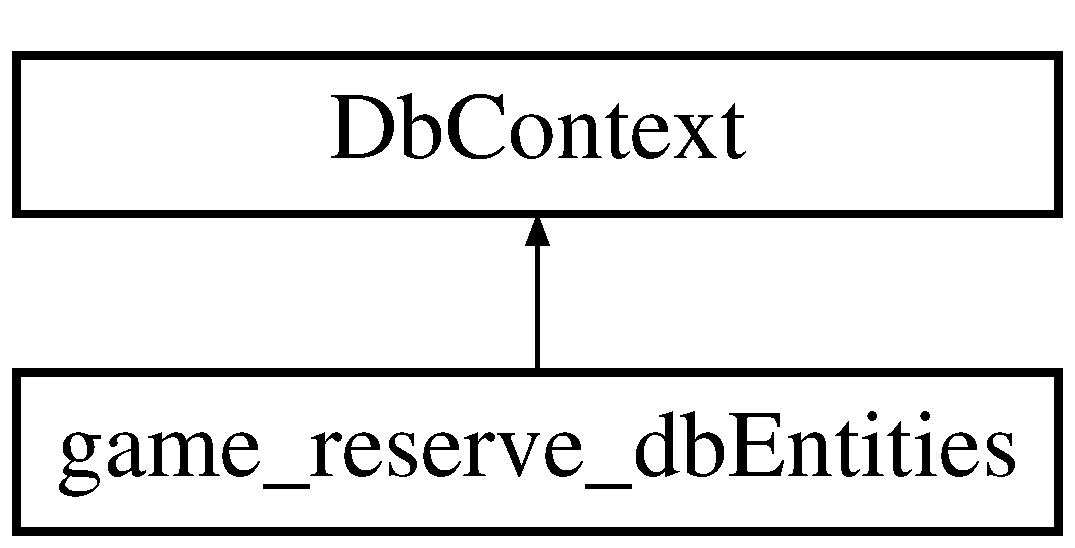
\includegraphics[height=2.000000cm]{classWildLifeTracker_1_1game__reserve__dbEntities}
\end{center}
\end{figure}
\subsection*{Public Member Functions}
\begin{DoxyCompactItemize}
\item 
\hyperlink{classWildLifeTracker_1_1game__reserve__dbEntities_a6075f6593be0d53a6314ed33bbe75cdf}{game\+\_\+reserve\+\_\+db\+Entities} ()
\end{DoxyCompactItemize}
\subsection*{Protected Member Functions}
\begin{DoxyCompactItemize}
\item 
override void \hyperlink{classWildLifeTracker_1_1game__reserve__dbEntities_a9161eb4f8fe83c74aab42d8fcde1fb10}{On\+Model\+Creating} (Db\+Model\+Builder model\+Builder)
\end{DoxyCompactItemize}
\subsection*{Properties}
\begin{DoxyCompactItemize}
\item 
virtual Db\+Set$<$ \hyperlink{classWildLifeTracker_1_1tblanimal}{tblanimal} $>$ \hyperlink{classWildLifeTracker_1_1game__reserve__dbEntities_a89197034701cb1b73d5aefd7691de04d}{tblanimals}\hspace{0.3cm}{\ttfamily  \mbox{[}get, set\mbox{]}}
\item 
virtual Db\+Set$<$ \hyperlink{classWildLifeTracker_1_1tblcategory}{tblcategory} $>$ \hyperlink{classWildLifeTracker_1_1game__reserve__dbEntities_a5aaa1d41e5de932e9cedbefefde0fa04}{tblcategories}\hspace{0.3cm}{\ttfamily  \mbox{[}get, set\mbox{]}}
\item 
virtual Db\+Set$<$ \hyperlink{classWildLifeTracker_1_1tblgpstracking}{tblgpstracking} $>$ \hyperlink{classWildLifeTracker_1_1game__reserve__dbEntities_a9b22490ada233f3325165fbd2acebeec}{tblgpstrackings}\hspace{0.3cm}{\ttfamily  \mbox{[}get, set\mbox{]}}
\end{DoxyCompactItemize}


\subsection{Constructor \& Destructor Documentation}
\mbox{\Hypertarget{classWildLifeTracker_1_1game__reserve__dbEntities_a6075f6593be0d53a6314ed33bbe75cdf}\label{classWildLifeTracker_1_1game__reserve__dbEntities_a6075f6593be0d53a6314ed33bbe75cdf}} 
\index{Wild\+Life\+Tracker\+::game\+\_\+reserve\+\_\+db\+Entities@{Wild\+Life\+Tracker\+::game\+\_\+reserve\+\_\+db\+Entities}!game\+\_\+reserve\+\_\+db\+Entities@{game\+\_\+reserve\+\_\+db\+Entities}}
\index{game\+\_\+reserve\+\_\+db\+Entities@{game\+\_\+reserve\+\_\+db\+Entities}!Wild\+Life\+Tracker\+::game\+\_\+reserve\+\_\+db\+Entities@{Wild\+Life\+Tracker\+::game\+\_\+reserve\+\_\+db\+Entities}}
\subsubsection{\texorpdfstring{game\+\_\+reserve\+\_\+db\+Entities()}{game\_reserve\_dbEntities()}}
{\footnotesize\ttfamily \hyperlink{classWildLifeTracker_1_1game__reserve__dbEntities}{game\+\_\+reserve\+\_\+db\+Entities} (\begin{DoxyParamCaption}{ }\end{DoxyParamCaption})\hspace{0.3cm}{\ttfamily [inline]}}



\subsection{Member Function Documentation}
\mbox{\Hypertarget{classWildLifeTracker_1_1game__reserve__dbEntities_a9161eb4f8fe83c74aab42d8fcde1fb10}\label{classWildLifeTracker_1_1game__reserve__dbEntities_a9161eb4f8fe83c74aab42d8fcde1fb10}} 
\index{Wild\+Life\+Tracker\+::game\+\_\+reserve\+\_\+db\+Entities@{Wild\+Life\+Tracker\+::game\+\_\+reserve\+\_\+db\+Entities}!On\+Model\+Creating@{On\+Model\+Creating}}
\index{On\+Model\+Creating@{On\+Model\+Creating}!Wild\+Life\+Tracker\+::game\+\_\+reserve\+\_\+db\+Entities@{Wild\+Life\+Tracker\+::game\+\_\+reserve\+\_\+db\+Entities}}
\subsubsection{\texorpdfstring{On\+Model\+Creating()}{OnModelCreating()}}
{\footnotesize\ttfamily override void On\+Model\+Creating (\begin{DoxyParamCaption}\item[{Db\+Model\+Builder}]{model\+Builder }\end{DoxyParamCaption})\hspace{0.3cm}{\ttfamily [inline]}, {\ttfamily [protected]}}



\subsection{Property Documentation}
\mbox{\Hypertarget{classWildLifeTracker_1_1game__reserve__dbEntities_a89197034701cb1b73d5aefd7691de04d}\label{classWildLifeTracker_1_1game__reserve__dbEntities_a89197034701cb1b73d5aefd7691de04d}} 
\index{Wild\+Life\+Tracker\+::game\+\_\+reserve\+\_\+db\+Entities@{Wild\+Life\+Tracker\+::game\+\_\+reserve\+\_\+db\+Entities}!tblanimals@{tblanimals}}
\index{tblanimals@{tblanimals}!Wild\+Life\+Tracker\+::game\+\_\+reserve\+\_\+db\+Entities@{Wild\+Life\+Tracker\+::game\+\_\+reserve\+\_\+db\+Entities}}
\subsubsection{\texorpdfstring{tblanimals}{tblanimals}}
{\footnotesize\ttfamily virtual Db\+Set$<$\hyperlink{classWildLifeTracker_1_1tblanimal}{tblanimal}$>$ tblanimals\hspace{0.3cm}{\ttfamily [get]}, {\ttfamily [set]}}

\mbox{\Hypertarget{classWildLifeTracker_1_1game__reserve__dbEntities_a5aaa1d41e5de932e9cedbefefde0fa04}\label{classWildLifeTracker_1_1game__reserve__dbEntities_a5aaa1d41e5de932e9cedbefefde0fa04}} 
\index{Wild\+Life\+Tracker\+::game\+\_\+reserve\+\_\+db\+Entities@{Wild\+Life\+Tracker\+::game\+\_\+reserve\+\_\+db\+Entities}!tblcategories@{tblcategories}}
\index{tblcategories@{tblcategories}!Wild\+Life\+Tracker\+::game\+\_\+reserve\+\_\+db\+Entities@{Wild\+Life\+Tracker\+::game\+\_\+reserve\+\_\+db\+Entities}}
\subsubsection{\texorpdfstring{tblcategories}{tblcategories}}
{\footnotesize\ttfamily virtual Db\+Set$<$\hyperlink{classWildLifeTracker_1_1tblcategory}{tblcategory}$>$ tblcategories\hspace{0.3cm}{\ttfamily [get]}, {\ttfamily [set]}}

\mbox{\Hypertarget{classWildLifeTracker_1_1game__reserve__dbEntities_a9b22490ada233f3325165fbd2acebeec}\label{classWildLifeTracker_1_1game__reserve__dbEntities_a9b22490ada233f3325165fbd2acebeec}} 
\index{Wild\+Life\+Tracker\+::game\+\_\+reserve\+\_\+db\+Entities@{Wild\+Life\+Tracker\+::game\+\_\+reserve\+\_\+db\+Entities}!tblgpstrackings@{tblgpstrackings}}
\index{tblgpstrackings@{tblgpstrackings}!Wild\+Life\+Tracker\+::game\+\_\+reserve\+\_\+db\+Entities@{Wild\+Life\+Tracker\+::game\+\_\+reserve\+\_\+db\+Entities}}
\subsubsection{\texorpdfstring{tblgpstrackings}{tblgpstrackings}}
{\footnotesize\ttfamily virtual Db\+Set$<$\hyperlink{classWildLifeTracker_1_1tblgpstracking}{tblgpstracking}$>$ tblgpstrackings\hspace{0.3cm}{\ttfamily [get]}, {\ttfamily [set]}}



The documentation for this class was generated from the following file\+:\begin{DoxyCompactItemize}
\item 
Wild\+Life\+Tracker/\hyperlink{DbModels_8Context_8cs}{Db\+Models.\+Context.\+cs}\end{DoxyCompactItemize}

\hypertarget{interfaceWildLifeTracker_1_1ICategoryService}{}\section{I\+Category\+Service}
\label{interfaceWildLifeTracker_1_1ICategoryService}\index{I\+Category\+Service@{I\+Category\+Service}}


The interface exposes all the A\+P\+Is for category details  


Inheritance diagram for I\+Category\+Service\+:\begin{figure}[H]
\begin{center}
\leavevmode
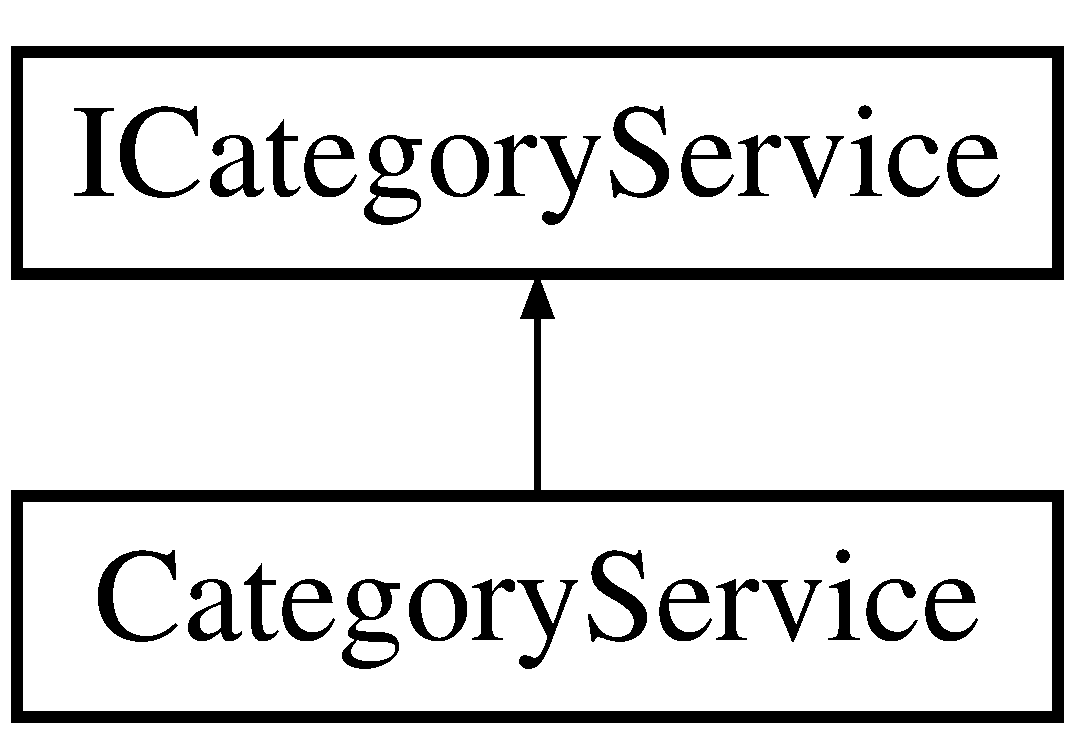
\includegraphics[height=2.000000cm]{interfaceWildLifeTracker_1_1ICategoryService}
\end{center}
\end{figure}
\subsection*{Public Member Functions}
\begin{DoxyCompactItemize}
\item 
\hyperlink{classWildLifeTracker_1_1Response_1_1CategoryResponse}{Category\+Response} \hyperlink{interfaceWildLifeTracker_1_1ICategoryService_ab22f6cdfb39adc2607dc86cb100889fc}{Add\+Category} (\hyperlink{classWildLifeTracker_1_1Models_1_1Category}{Category} category\+Details)
\begin{DoxyCompactList}\small\item\em Adds a new category. 
\begin{DoxyParams}{Parameters}
{\em category\+Details} & The category details to be added\\
\hline
\end{DoxyParams}
\begin{DoxyReturn}{Returns}
Returns the category details for the newly created category or throws Exception if there is error
\end{DoxyReturn}
\end{DoxyCompactList}\item 
\hyperlink{classWildLifeTracker_1_1Response_1_1CategoryResponse}{Category\+Response} \hyperlink{interfaceWildLifeTracker_1_1ICategoryService_a6479e2a6945b14d40e8c57642e9d2665}{Delete\+Category} (string category\+Id)
\begin{DoxyCompactList}\small\item\em Delete the category details. 
\begin{DoxyParams}{Parameters}
{\em category\+Id} & the category id\\
\hline
\end{DoxyParams}
\begin{DoxyReturn}{Returns}
Returns the animal details of animal that is deleted
\end{DoxyReturn}
\end{DoxyCompactList}\item 
\hyperlink{classWildLifeTracker_1_1Response_1_1CategoryResponse}{Category\+Response} \hyperlink{interfaceWildLifeTracker_1_1ICategoryService_af5ed969c812807a721f06819c9b22356}{Get\+Categories} ()
\begin{DoxyCompactList}\small\item\em Retrieves all the categories. \begin{DoxyReturn}{Returns}
Returns all the categories details
\end{DoxyReturn}
\end{DoxyCompactList}\item 
\hyperlink{classWildLifeTracker_1_1Response_1_1CategoryResponse}{Category\+Response} \hyperlink{interfaceWildLifeTracker_1_1ICategoryService_ac989af6747cc8b28f508ef7a4645d22f}{Get\+Category} (string category\+Id)
\begin{DoxyCompactList}\small\item\em Retrieves the category details when category\+Id is specified. 
\begin{DoxyParams}{Parameters}
{\em category\+Id} & the category id\\
\hline
\end{DoxyParams}
\begin{DoxyReturn}{Returns}
Returns the categories detail for given category Id
\end{DoxyReturn}
\end{DoxyCompactList}\item 
\hyperlink{classWildLifeTracker_1_1Response_1_1CategoryResponse}{Category\+Response} \hyperlink{interfaceWildLifeTracker_1_1ICategoryService_adbaa7c66fd8789233e4d6f91ab3a4a2f}{Update\+Category} (string category\+Id, \hyperlink{classWildLifeTracker_1_1Models_1_1Category}{Category} category\+Details)
\begin{DoxyCompactList}\small\item\em Update an category details. 
\begin{DoxyParams}{Parameters}
{\em category\+Id} & the category id\\
\hline
\end{DoxyParams}
/// 
\begin{DoxyParams}{Parameters}
{\em category\+Details} & the category details\\
\hline
\end{DoxyParams}
\begin{DoxyReturn}{Returns}
Returns the category details of updated category
\end{DoxyReturn}
\end{DoxyCompactList}\end{DoxyCompactItemize}


\subsection{Detailed Description}
The interface exposes all the A\+P\+Is for category details 



\subsection{Member Function Documentation}
\mbox{\Hypertarget{interfaceWildLifeTracker_1_1ICategoryService_ab22f6cdfb39adc2607dc86cb100889fc}\label{interfaceWildLifeTracker_1_1ICategoryService_ab22f6cdfb39adc2607dc86cb100889fc}} 
\index{Wild\+Life\+Tracker\+::\+I\+Category\+Service@{Wild\+Life\+Tracker\+::\+I\+Category\+Service}!Add\+Category@{Add\+Category}}
\index{Add\+Category@{Add\+Category}!Wild\+Life\+Tracker\+::\+I\+Category\+Service@{Wild\+Life\+Tracker\+::\+I\+Category\+Service}}
\subsubsection{\texorpdfstring{Add\+Category()}{AddCategory()}}
{\footnotesize\ttfamily \hyperlink{classWildLifeTracker_1_1Response_1_1CategoryResponse}{Category\+Response} Add\+Category (\begin{DoxyParamCaption}\item[{\hyperlink{classWildLifeTracker_1_1Models_1_1Category}{Category}}]{category\+Details }\end{DoxyParamCaption})}



Adds a new category. 
\begin{DoxyParams}{Parameters}
{\em category\+Details} & The category details to be added\\
\hline
\end{DoxyParams}
\begin{DoxyReturn}{Returns}
Returns the category details for the newly created category or throws Exception if there is error
\end{DoxyReturn}




Implemented in \hyperlink{classWildLifeTracker_1_1CategoryService_ab22f6cdfb39adc2607dc86cb100889fc}{Category\+Service}.

\mbox{\Hypertarget{interfaceWildLifeTracker_1_1ICategoryService_a6479e2a6945b14d40e8c57642e9d2665}\label{interfaceWildLifeTracker_1_1ICategoryService_a6479e2a6945b14d40e8c57642e9d2665}} 
\index{Wild\+Life\+Tracker\+::\+I\+Category\+Service@{Wild\+Life\+Tracker\+::\+I\+Category\+Service}!Delete\+Category@{Delete\+Category}}
\index{Delete\+Category@{Delete\+Category}!Wild\+Life\+Tracker\+::\+I\+Category\+Service@{Wild\+Life\+Tracker\+::\+I\+Category\+Service}}
\subsubsection{\texorpdfstring{Delete\+Category()}{DeleteCategory()}}
{\footnotesize\ttfamily \hyperlink{classWildLifeTracker_1_1Response_1_1CategoryResponse}{Category\+Response} Delete\+Category (\begin{DoxyParamCaption}\item[{string}]{category\+Id }\end{DoxyParamCaption})}



Delete the category details. 
\begin{DoxyParams}{Parameters}
{\em category\+Id} & the category id\\
\hline
\end{DoxyParams}
\begin{DoxyReturn}{Returns}
Returns the animal details of animal that is deleted
\end{DoxyReturn}




Implemented in \hyperlink{classWildLifeTracker_1_1CategoryService_a6479e2a6945b14d40e8c57642e9d2665}{Category\+Service}.

\mbox{\Hypertarget{interfaceWildLifeTracker_1_1ICategoryService_af5ed969c812807a721f06819c9b22356}\label{interfaceWildLifeTracker_1_1ICategoryService_af5ed969c812807a721f06819c9b22356}} 
\index{Wild\+Life\+Tracker\+::\+I\+Category\+Service@{Wild\+Life\+Tracker\+::\+I\+Category\+Service}!Get\+Categories@{Get\+Categories}}
\index{Get\+Categories@{Get\+Categories}!Wild\+Life\+Tracker\+::\+I\+Category\+Service@{Wild\+Life\+Tracker\+::\+I\+Category\+Service}}
\subsubsection{\texorpdfstring{Get\+Categories()}{GetCategories()}}
{\footnotesize\ttfamily \hyperlink{classWildLifeTracker_1_1Response_1_1CategoryResponse}{Category\+Response} Get\+Categories (\begin{DoxyParamCaption}{ }\end{DoxyParamCaption})}



Retrieves all the categories. \begin{DoxyReturn}{Returns}
Returns all the categories details
\end{DoxyReturn}




Implemented in \hyperlink{classWildLifeTracker_1_1CategoryService_af5ed969c812807a721f06819c9b22356}{Category\+Service}.

\mbox{\Hypertarget{interfaceWildLifeTracker_1_1ICategoryService_ac989af6747cc8b28f508ef7a4645d22f}\label{interfaceWildLifeTracker_1_1ICategoryService_ac989af6747cc8b28f508ef7a4645d22f}} 
\index{Wild\+Life\+Tracker\+::\+I\+Category\+Service@{Wild\+Life\+Tracker\+::\+I\+Category\+Service}!Get\+Category@{Get\+Category}}
\index{Get\+Category@{Get\+Category}!Wild\+Life\+Tracker\+::\+I\+Category\+Service@{Wild\+Life\+Tracker\+::\+I\+Category\+Service}}
\subsubsection{\texorpdfstring{Get\+Category()}{GetCategory()}}
{\footnotesize\ttfamily \hyperlink{classWildLifeTracker_1_1Response_1_1CategoryResponse}{Category\+Response} Get\+Category (\begin{DoxyParamCaption}\item[{string}]{category\+Id }\end{DoxyParamCaption})}



Retrieves the category details when category\+Id is specified. 
\begin{DoxyParams}{Parameters}
{\em category\+Id} & the category id\\
\hline
\end{DoxyParams}
\begin{DoxyReturn}{Returns}
Returns the categories detail for given category Id
\end{DoxyReturn}




Implemented in \hyperlink{classWildLifeTracker_1_1CategoryService_ac989af6747cc8b28f508ef7a4645d22f}{Category\+Service}.

\mbox{\Hypertarget{interfaceWildLifeTracker_1_1ICategoryService_adbaa7c66fd8789233e4d6f91ab3a4a2f}\label{interfaceWildLifeTracker_1_1ICategoryService_adbaa7c66fd8789233e4d6f91ab3a4a2f}} 
\index{Wild\+Life\+Tracker\+::\+I\+Category\+Service@{Wild\+Life\+Tracker\+::\+I\+Category\+Service}!Update\+Category@{Update\+Category}}
\index{Update\+Category@{Update\+Category}!Wild\+Life\+Tracker\+::\+I\+Category\+Service@{Wild\+Life\+Tracker\+::\+I\+Category\+Service}}
\subsubsection{\texorpdfstring{Update\+Category()}{UpdateCategory()}}
{\footnotesize\ttfamily \hyperlink{classWildLifeTracker_1_1Response_1_1CategoryResponse}{Category\+Response} Update\+Category (\begin{DoxyParamCaption}\item[{string}]{category\+Id,  }\item[{\hyperlink{classWildLifeTracker_1_1Models_1_1Category}{Category}}]{category\+Details }\end{DoxyParamCaption})}



Update an category details. 
\begin{DoxyParams}{Parameters}
{\em category\+Id} & the category id\\
\hline
\end{DoxyParams}
/// 
\begin{DoxyParams}{Parameters}
{\em category\+Details} & the category details\\
\hline
\end{DoxyParams}
\begin{DoxyReturn}{Returns}
Returns the category details of updated category
\end{DoxyReturn}




Implemented in \hyperlink{classWildLifeTracker_1_1CategoryService_adbaa7c66fd8789233e4d6f91ab3a4a2f}{Category\+Service}.



The documentation for this interface was generated from the following file\+:\begin{DoxyCompactItemize}
\item 
Wild\+Life\+Tracker/\+Services/\hyperlink{ICategoryServices_8cs}{I\+Category\+Services.\+cs}\end{DoxyCompactItemize}

\hypertarget{classWildLifeTracker_1_1Models_1_1Animal}{}\section{Animal}
\label{classWildLifeTracker_1_1Models_1_1Animal}\index{Animal@{Animal}}
\subsection*{Properties}
\begin{DoxyCompactItemize}
\item 
int \hyperlink{classWildLifeTracker_1_1Models_1_1Animal_a99787b9867ae390df467a99040589a55}{animal\+Id}\hspace{0.3cm}{\ttfamily  \mbox{[}get, set\mbox{]}}
\begin{DoxyCompactList}\small\item\em The model is for \hyperlink{classWildLifeTracker_1_1Models_1_1Animal}{Animal} Operations having animal Id, name, G\+PS device ID \end{DoxyCompactList}\item 
string \hyperlink{classWildLifeTracker_1_1Models_1_1Animal_afd38ba6641283469fc9e94212467f9a2}{animal\+Name}\hspace{0.3cm}{\ttfamily  \mbox{[}get, set\mbox{]}}
\item 
int \hyperlink{classWildLifeTracker_1_1Models_1_1Animal_a423f91c56dc35040d661cfbe357f7c78}{category\+Id}\hspace{0.3cm}{\ttfamily  \mbox{[}get, set\mbox{]}}
\item 
System.\+Date\+Time \hyperlink{classWildLifeTracker_1_1Models_1_1Animal_a0da6329d5fbb1b91739557ad49ece9c0}{created\+At}\hspace{0.3cm}{\ttfamily  \mbox{[}get, set\mbox{]}}
\item 
string \hyperlink{classWildLifeTracker_1_1Models_1_1Animal_a073b88a9702ca0513fa534f58a048070}{gps\+Device\+Id}\hspace{0.3cm}{\ttfamily  \mbox{[}get, set\mbox{]}}
\end{DoxyCompactItemize}


\subsection{Property Documentation}
\mbox{\Hypertarget{classWildLifeTracker_1_1Models_1_1Animal_a99787b9867ae390df467a99040589a55}\label{classWildLifeTracker_1_1Models_1_1Animal_a99787b9867ae390df467a99040589a55}} 
\index{Wild\+Life\+Tracker\+::\+Models\+::\+Animal@{Wild\+Life\+Tracker\+::\+Models\+::\+Animal}!animal\+Id@{animal\+Id}}
\index{animal\+Id@{animal\+Id}!Wild\+Life\+Tracker\+::\+Models\+::\+Animal@{Wild\+Life\+Tracker\+::\+Models\+::\+Animal}}
\subsubsection{\texorpdfstring{animal\+Id}{animalId}}
{\footnotesize\ttfamily int animal\+Id\hspace{0.3cm}{\ttfamily [get]}, {\ttfamily [set]}}



The model is for \hyperlink{classWildLifeTracker_1_1Models_1_1Animal}{Animal} Operations having animal Id, name, G\+PS device ID 

\mbox{\Hypertarget{classWildLifeTracker_1_1Models_1_1Animal_afd38ba6641283469fc9e94212467f9a2}\label{classWildLifeTracker_1_1Models_1_1Animal_afd38ba6641283469fc9e94212467f9a2}} 
\index{Wild\+Life\+Tracker\+::\+Models\+::\+Animal@{Wild\+Life\+Tracker\+::\+Models\+::\+Animal}!animal\+Name@{animal\+Name}}
\index{animal\+Name@{animal\+Name}!Wild\+Life\+Tracker\+::\+Models\+::\+Animal@{Wild\+Life\+Tracker\+::\+Models\+::\+Animal}}
\subsubsection{\texorpdfstring{animal\+Name}{animalName}}
{\footnotesize\ttfamily string animal\+Name\hspace{0.3cm}{\ttfamily [get]}, {\ttfamily [set]}}

\mbox{\Hypertarget{classWildLifeTracker_1_1Models_1_1Animal_a423f91c56dc35040d661cfbe357f7c78}\label{classWildLifeTracker_1_1Models_1_1Animal_a423f91c56dc35040d661cfbe357f7c78}} 
\index{Wild\+Life\+Tracker\+::\+Models\+::\+Animal@{Wild\+Life\+Tracker\+::\+Models\+::\+Animal}!category\+Id@{category\+Id}}
\index{category\+Id@{category\+Id}!Wild\+Life\+Tracker\+::\+Models\+::\+Animal@{Wild\+Life\+Tracker\+::\+Models\+::\+Animal}}
\subsubsection{\texorpdfstring{category\+Id}{categoryId}}
{\footnotesize\ttfamily int category\+Id\hspace{0.3cm}{\ttfamily [get]}, {\ttfamily [set]}}

\mbox{\Hypertarget{classWildLifeTracker_1_1Models_1_1Animal_a0da6329d5fbb1b91739557ad49ece9c0}\label{classWildLifeTracker_1_1Models_1_1Animal_a0da6329d5fbb1b91739557ad49ece9c0}} 
\index{Wild\+Life\+Tracker\+::\+Models\+::\+Animal@{Wild\+Life\+Tracker\+::\+Models\+::\+Animal}!created\+At@{created\+At}}
\index{created\+At@{created\+At}!Wild\+Life\+Tracker\+::\+Models\+::\+Animal@{Wild\+Life\+Tracker\+::\+Models\+::\+Animal}}
\subsubsection{\texorpdfstring{created\+At}{createdAt}}
{\footnotesize\ttfamily System.\+Date\+Time created\+At\hspace{0.3cm}{\ttfamily [get]}, {\ttfamily [set]}}

\mbox{\Hypertarget{classWildLifeTracker_1_1Models_1_1Animal_a073b88a9702ca0513fa534f58a048070}\label{classWildLifeTracker_1_1Models_1_1Animal_a073b88a9702ca0513fa534f58a048070}} 
\index{Wild\+Life\+Tracker\+::\+Models\+::\+Animal@{Wild\+Life\+Tracker\+::\+Models\+::\+Animal}!gps\+Device\+Id@{gps\+Device\+Id}}
\index{gps\+Device\+Id@{gps\+Device\+Id}!Wild\+Life\+Tracker\+::\+Models\+::\+Animal@{Wild\+Life\+Tracker\+::\+Models\+::\+Animal}}
\subsubsection{\texorpdfstring{gps\+Device\+Id}{gpsDeviceId}}
{\footnotesize\ttfamily string gps\+Device\+Id\hspace{0.3cm}{\ttfamily [get]}, {\ttfamily [set]}}



The documentation for this class was generated from the following file\+:\begin{DoxyCompactItemize}
\item 
Wild\+Life\+Tracker/\+Models/\hyperlink{Animal_8cs}{Animal.\+cs}\end{DoxyCompactItemize}

\hypertarget{classWildLifeTracker_1_1Models_1_1AnimalCount}{}\section{Animal\+Count}
\label{classWildLifeTracker_1_1Models_1_1AnimalCount}\index{Animal\+Count@{Animal\+Count}}
\subsection*{Properties}
\begin{DoxyCompactItemize}
\item 
int \hyperlink{classWildLifeTracker_1_1Models_1_1AnimalCount_a423f91c56dc35040d661cfbe357f7c78}{category\+Id}\hspace{0.3cm}{\ttfamily  \mbox{[}get, set\mbox{]}}
\begin{DoxyCompactList}\small\item\em The model is for \hyperlink{classWildLifeTracker_1_1Models_1_1Animal}{Animal} Count having the details of animals and keep the count of it \end{DoxyCompactList}\item 
string \hyperlink{classWildLifeTracker_1_1Models_1_1AnimalCount_a1eca787c85e1bc45b49bbd281d4106fd}{category\+Name}\hspace{0.3cm}{\ttfamily  \mbox{[}get, set\mbox{]}}
\item 
string \hyperlink{classWildLifeTracker_1_1Models_1_1AnimalCount_a0ecdefcc99a4b41b1ef3a04167756366}{color\+Indication}\hspace{0.3cm}{\ttfamily  \mbox{[}get, set\mbox{]}}
\item 
int \hyperlink{classWildLifeTracker_1_1Models_1_1AnimalCount_af2a3c76f434001a3f47c287cc16f04ff}{total\+Animals}\hspace{0.3cm}{\ttfamily  \mbox{[}get, set\mbox{]}}
\end{DoxyCompactItemize}


\subsection{Property Documentation}
\mbox{\Hypertarget{classWildLifeTracker_1_1Models_1_1AnimalCount_a423f91c56dc35040d661cfbe357f7c78}\label{classWildLifeTracker_1_1Models_1_1AnimalCount_a423f91c56dc35040d661cfbe357f7c78}} 
\index{Wild\+Life\+Tracker\+::\+Models\+::\+Animal\+Count@{Wild\+Life\+Tracker\+::\+Models\+::\+Animal\+Count}!category\+Id@{category\+Id}}
\index{category\+Id@{category\+Id}!Wild\+Life\+Tracker\+::\+Models\+::\+Animal\+Count@{Wild\+Life\+Tracker\+::\+Models\+::\+Animal\+Count}}
\subsubsection{\texorpdfstring{category\+Id}{categoryId}}
{\footnotesize\ttfamily int category\+Id\hspace{0.3cm}{\ttfamily [get]}, {\ttfamily [set]}}



The model is for \hyperlink{classWildLifeTracker_1_1Models_1_1Animal}{Animal} Count having the details of animals and keep the count of it 

\mbox{\Hypertarget{classWildLifeTracker_1_1Models_1_1AnimalCount_a1eca787c85e1bc45b49bbd281d4106fd}\label{classWildLifeTracker_1_1Models_1_1AnimalCount_a1eca787c85e1bc45b49bbd281d4106fd}} 
\index{Wild\+Life\+Tracker\+::\+Models\+::\+Animal\+Count@{Wild\+Life\+Tracker\+::\+Models\+::\+Animal\+Count}!category\+Name@{category\+Name}}
\index{category\+Name@{category\+Name}!Wild\+Life\+Tracker\+::\+Models\+::\+Animal\+Count@{Wild\+Life\+Tracker\+::\+Models\+::\+Animal\+Count}}
\subsubsection{\texorpdfstring{category\+Name}{categoryName}}
{\footnotesize\ttfamily string category\+Name\hspace{0.3cm}{\ttfamily [get]}, {\ttfamily [set]}}

\mbox{\Hypertarget{classWildLifeTracker_1_1Models_1_1AnimalCount_a0ecdefcc99a4b41b1ef3a04167756366}\label{classWildLifeTracker_1_1Models_1_1AnimalCount_a0ecdefcc99a4b41b1ef3a04167756366}} 
\index{Wild\+Life\+Tracker\+::\+Models\+::\+Animal\+Count@{Wild\+Life\+Tracker\+::\+Models\+::\+Animal\+Count}!color\+Indication@{color\+Indication}}
\index{color\+Indication@{color\+Indication}!Wild\+Life\+Tracker\+::\+Models\+::\+Animal\+Count@{Wild\+Life\+Tracker\+::\+Models\+::\+Animal\+Count}}
\subsubsection{\texorpdfstring{color\+Indication}{colorIndication}}
{\footnotesize\ttfamily string color\+Indication\hspace{0.3cm}{\ttfamily [get]}, {\ttfamily [set]}}

\mbox{\Hypertarget{classWildLifeTracker_1_1Models_1_1AnimalCount_af2a3c76f434001a3f47c287cc16f04ff}\label{classWildLifeTracker_1_1Models_1_1AnimalCount_af2a3c76f434001a3f47c287cc16f04ff}} 
\index{Wild\+Life\+Tracker\+::\+Models\+::\+Animal\+Count@{Wild\+Life\+Tracker\+::\+Models\+::\+Animal\+Count}!total\+Animals@{total\+Animals}}
\index{total\+Animals@{total\+Animals}!Wild\+Life\+Tracker\+::\+Models\+::\+Animal\+Count@{Wild\+Life\+Tracker\+::\+Models\+::\+Animal\+Count}}
\subsubsection{\texorpdfstring{total\+Animals}{totalAnimals}}
{\footnotesize\ttfamily int total\+Animals\hspace{0.3cm}{\ttfamily [get]}, {\ttfamily [set]}}



The documentation for this class was generated from the following file\+:\begin{DoxyCompactItemize}
\item 
Wild\+Life\+Tracker/\+Models/\hyperlink{AnimalCount_8cs}{Animal\+Count.\+cs}\end{DoxyCompactItemize}

\hypertarget{classWildLifeTracker_1_1Models_1_1Category}{}\section{Category}
\label{classWildLifeTracker_1_1Models_1_1Category}\index{Category@{Category}}
\subsection*{Properties}
\begin{DoxyCompactItemize}
\item 
string \hyperlink{classWildLifeTracker_1_1Models_1_1Category_ae992743f1fc0d9386b609d8871a4bd6b}{category\+Desc}\hspace{0.3cm}{\ttfamily  \mbox{[}get, set\mbox{]}}
\item 
int \hyperlink{classWildLifeTracker_1_1Models_1_1Category_a423f91c56dc35040d661cfbe357f7c78}{category\+Id}\hspace{0.3cm}{\ttfamily  \mbox{[}get, set\mbox{]}}
\begin{DoxyCompactList}\small\item\em The model is for \hyperlink{classWildLifeTracker_1_1Models_1_1Category}{Category} Operations having category Id, name \end{DoxyCompactList}\item 
string \hyperlink{classWildLifeTracker_1_1Models_1_1Category_a1eca787c85e1bc45b49bbd281d4106fd}{category\+Name}\hspace{0.3cm}{\ttfamily  \mbox{[}get, set\mbox{]}}
\item 
string \hyperlink{classWildLifeTracker_1_1Models_1_1Category_a0ecdefcc99a4b41b1ef3a04167756366}{color\+Indication}\hspace{0.3cm}{\ttfamily  \mbox{[}get, set\mbox{]}}
\end{DoxyCompactItemize}


\subsection{Property Documentation}
\mbox{\Hypertarget{classWildLifeTracker_1_1Models_1_1Category_ae992743f1fc0d9386b609d8871a4bd6b}\label{classWildLifeTracker_1_1Models_1_1Category_ae992743f1fc0d9386b609d8871a4bd6b}} 
\index{Wild\+Life\+Tracker\+::\+Models\+::\+Category@{Wild\+Life\+Tracker\+::\+Models\+::\+Category}!category\+Desc@{category\+Desc}}
\index{category\+Desc@{category\+Desc}!Wild\+Life\+Tracker\+::\+Models\+::\+Category@{Wild\+Life\+Tracker\+::\+Models\+::\+Category}}
\subsubsection{\texorpdfstring{category\+Desc}{categoryDesc}}
{\footnotesize\ttfamily string category\+Desc\hspace{0.3cm}{\ttfamily [get]}, {\ttfamily [set]}}

\mbox{\Hypertarget{classWildLifeTracker_1_1Models_1_1Category_a423f91c56dc35040d661cfbe357f7c78}\label{classWildLifeTracker_1_1Models_1_1Category_a423f91c56dc35040d661cfbe357f7c78}} 
\index{Wild\+Life\+Tracker\+::\+Models\+::\+Category@{Wild\+Life\+Tracker\+::\+Models\+::\+Category}!category\+Id@{category\+Id}}
\index{category\+Id@{category\+Id}!Wild\+Life\+Tracker\+::\+Models\+::\+Category@{Wild\+Life\+Tracker\+::\+Models\+::\+Category}}
\subsubsection{\texorpdfstring{category\+Id}{categoryId}}
{\footnotesize\ttfamily int category\+Id\hspace{0.3cm}{\ttfamily [get]}, {\ttfamily [set]}}



The model is for \hyperlink{classWildLifeTracker_1_1Models_1_1Category}{Category} Operations having category Id, name 

\mbox{\Hypertarget{classWildLifeTracker_1_1Models_1_1Category_a1eca787c85e1bc45b49bbd281d4106fd}\label{classWildLifeTracker_1_1Models_1_1Category_a1eca787c85e1bc45b49bbd281d4106fd}} 
\index{Wild\+Life\+Tracker\+::\+Models\+::\+Category@{Wild\+Life\+Tracker\+::\+Models\+::\+Category}!category\+Name@{category\+Name}}
\index{category\+Name@{category\+Name}!Wild\+Life\+Tracker\+::\+Models\+::\+Category@{Wild\+Life\+Tracker\+::\+Models\+::\+Category}}
\subsubsection{\texorpdfstring{category\+Name}{categoryName}}
{\footnotesize\ttfamily string category\+Name\hspace{0.3cm}{\ttfamily [get]}, {\ttfamily [set]}}

\mbox{\Hypertarget{classWildLifeTracker_1_1Models_1_1Category_a0ecdefcc99a4b41b1ef3a04167756366}\label{classWildLifeTracker_1_1Models_1_1Category_a0ecdefcc99a4b41b1ef3a04167756366}} 
\index{Wild\+Life\+Tracker\+::\+Models\+::\+Category@{Wild\+Life\+Tracker\+::\+Models\+::\+Category}!color\+Indication@{color\+Indication}}
\index{color\+Indication@{color\+Indication}!Wild\+Life\+Tracker\+::\+Models\+::\+Category@{Wild\+Life\+Tracker\+::\+Models\+::\+Category}}
\subsubsection{\texorpdfstring{color\+Indication}{colorIndication}}
{\footnotesize\ttfamily string color\+Indication\hspace{0.3cm}{\ttfamily [get]}, {\ttfamily [set]}}



The documentation for this class was generated from the following file\+:\begin{DoxyCompactItemize}
\item 
Wild\+Life\+Tracker/\+Models/\hyperlink{Category_8cs}{Category.\+cs}\end{DoxyCompactItemize}

\hypertarget{classWildLifeTracker_1_1Models_1_1GPSTrackingInfo}{}\section{G\+P\+S\+Tracking\+Info}
\label{classWildLifeTracker_1_1Models_1_1GPSTrackingInfo}\index{G\+P\+S\+Tracking\+Info@{G\+P\+S\+Tracking\+Info}}
\subsection*{Properties}
\begin{DoxyCompactItemize}
\item 
int \hyperlink{classWildLifeTracker_1_1Models_1_1GPSTrackingInfo_a99787b9867ae390df467a99040589a55}{animal\+Id}\hspace{0.3cm}{\ttfamily  \mbox{[}get, set\mbox{]}}
\item 
string \hyperlink{classWildLifeTracker_1_1Models_1_1GPSTrackingInfo_afd38ba6641283469fc9e94212467f9a2}{animal\+Name}\hspace{0.3cm}{\ttfamily  \mbox{[}get, set\mbox{]}}
\item 
int \hyperlink{classWildLifeTracker_1_1Models_1_1GPSTrackingInfo_a423f91c56dc35040d661cfbe357f7c78}{category\+Id}\hspace{0.3cm}{\ttfamily  \mbox{[}get, set\mbox{]}}
\item 
string \hyperlink{classWildLifeTracker_1_1Models_1_1GPSTrackingInfo_a1eca787c85e1bc45b49bbd281d4106fd}{category\+Name}\hspace{0.3cm}{\ttfamily  \mbox{[}get, set\mbox{]}}
\item 
string \hyperlink{classWildLifeTracker_1_1Models_1_1GPSTrackingInfo_a0ecdefcc99a4b41b1ef3a04167756366}{color\+Indication}\hspace{0.3cm}{\ttfamily  \mbox{[}get, set\mbox{]}}
\item 
System.\+Date\+Time \hyperlink{classWildLifeTracker_1_1Models_1_1GPSTrackingInfo_a0da6329d5fbb1b91739557ad49ece9c0}{created\+At}\hspace{0.3cm}{\ttfamily  \mbox{[}get, set\mbox{]}}
\item 
string \hyperlink{classWildLifeTracker_1_1Models_1_1GPSTrackingInfo_a073b88a9702ca0513fa534f58a048070}{gps\+Device\+Id}\hspace{0.3cm}{\ttfamily  \mbox{[}get, set\mbox{]}}
\item 
double \hyperlink{classWildLifeTracker_1_1Models_1_1GPSTrackingInfo_a76714bdbc5c536fa77dfb14533ff82a9}{latitude}\hspace{0.3cm}{\ttfamily  \mbox{[}get, set\mbox{]}}
\item 
double \hyperlink{classWildLifeTracker_1_1Models_1_1GPSTrackingInfo_ac155e35fdeebafc89723a51520fb9fe6}{longitude}\hspace{0.3cm}{\ttfamily  \mbox{[}get, set\mbox{]}}
\item 
int \hyperlink{classWildLifeTracker_1_1Models_1_1GPSTrackingInfo_a7291076f1fbf1ead00eb6c30cf33d943}{tracking\+Id}\hspace{0.3cm}{\ttfamily  \mbox{[}get, set\mbox{]}}
\begin{DoxyCompactList}\small\item\em The model is for Tracking Information Operations having tracking details. \end{DoxyCompactList}\end{DoxyCompactItemize}


\subsection{Property Documentation}
\mbox{\Hypertarget{classWildLifeTracker_1_1Models_1_1GPSTrackingInfo_a99787b9867ae390df467a99040589a55}\label{classWildLifeTracker_1_1Models_1_1GPSTrackingInfo_a99787b9867ae390df467a99040589a55}} 
\index{Wild\+Life\+Tracker\+::\+Models\+::\+G\+P\+S\+Tracking\+Info@{Wild\+Life\+Tracker\+::\+Models\+::\+G\+P\+S\+Tracking\+Info}!animal\+Id@{animal\+Id}}
\index{animal\+Id@{animal\+Id}!Wild\+Life\+Tracker\+::\+Models\+::\+G\+P\+S\+Tracking\+Info@{Wild\+Life\+Tracker\+::\+Models\+::\+G\+P\+S\+Tracking\+Info}}
\subsubsection{\texorpdfstring{animal\+Id}{animalId}}
{\footnotesize\ttfamily int animal\+Id\hspace{0.3cm}{\ttfamily [get]}, {\ttfamily [set]}}

\mbox{\Hypertarget{classWildLifeTracker_1_1Models_1_1GPSTrackingInfo_afd38ba6641283469fc9e94212467f9a2}\label{classWildLifeTracker_1_1Models_1_1GPSTrackingInfo_afd38ba6641283469fc9e94212467f9a2}} 
\index{Wild\+Life\+Tracker\+::\+Models\+::\+G\+P\+S\+Tracking\+Info@{Wild\+Life\+Tracker\+::\+Models\+::\+G\+P\+S\+Tracking\+Info}!animal\+Name@{animal\+Name}}
\index{animal\+Name@{animal\+Name}!Wild\+Life\+Tracker\+::\+Models\+::\+G\+P\+S\+Tracking\+Info@{Wild\+Life\+Tracker\+::\+Models\+::\+G\+P\+S\+Tracking\+Info}}
\subsubsection{\texorpdfstring{animal\+Name}{animalName}}
{\footnotesize\ttfamily string animal\+Name\hspace{0.3cm}{\ttfamily [get]}, {\ttfamily [set]}}

\mbox{\Hypertarget{classWildLifeTracker_1_1Models_1_1GPSTrackingInfo_a423f91c56dc35040d661cfbe357f7c78}\label{classWildLifeTracker_1_1Models_1_1GPSTrackingInfo_a423f91c56dc35040d661cfbe357f7c78}} 
\index{Wild\+Life\+Tracker\+::\+Models\+::\+G\+P\+S\+Tracking\+Info@{Wild\+Life\+Tracker\+::\+Models\+::\+G\+P\+S\+Tracking\+Info}!category\+Id@{category\+Id}}
\index{category\+Id@{category\+Id}!Wild\+Life\+Tracker\+::\+Models\+::\+G\+P\+S\+Tracking\+Info@{Wild\+Life\+Tracker\+::\+Models\+::\+G\+P\+S\+Tracking\+Info}}
\subsubsection{\texorpdfstring{category\+Id}{categoryId}}
{\footnotesize\ttfamily int category\+Id\hspace{0.3cm}{\ttfamily [get]}, {\ttfamily [set]}}

\mbox{\Hypertarget{classWildLifeTracker_1_1Models_1_1GPSTrackingInfo_a1eca787c85e1bc45b49bbd281d4106fd}\label{classWildLifeTracker_1_1Models_1_1GPSTrackingInfo_a1eca787c85e1bc45b49bbd281d4106fd}} 
\index{Wild\+Life\+Tracker\+::\+Models\+::\+G\+P\+S\+Tracking\+Info@{Wild\+Life\+Tracker\+::\+Models\+::\+G\+P\+S\+Tracking\+Info}!category\+Name@{category\+Name}}
\index{category\+Name@{category\+Name}!Wild\+Life\+Tracker\+::\+Models\+::\+G\+P\+S\+Tracking\+Info@{Wild\+Life\+Tracker\+::\+Models\+::\+G\+P\+S\+Tracking\+Info}}
\subsubsection{\texorpdfstring{category\+Name}{categoryName}}
{\footnotesize\ttfamily string category\+Name\hspace{0.3cm}{\ttfamily [get]}, {\ttfamily [set]}}

\mbox{\Hypertarget{classWildLifeTracker_1_1Models_1_1GPSTrackingInfo_a0ecdefcc99a4b41b1ef3a04167756366}\label{classWildLifeTracker_1_1Models_1_1GPSTrackingInfo_a0ecdefcc99a4b41b1ef3a04167756366}} 
\index{Wild\+Life\+Tracker\+::\+Models\+::\+G\+P\+S\+Tracking\+Info@{Wild\+Life\+Tracker\+::\+Models\+::\+G\+P\+S\+Tracking\+Info}!color\+Indication@{color\+Indication}}
\index{color\+Indication@{color\+Indication}!Wild\+Life\+Tracker\+::\+Models\+::\+G\+P\+S\+Tracking\+Info@{Wild\+Life\+Tracker\+::\+Models\+::\+G\+P\+S\+Tracking\+Info}}
\subsubsection{\texorpdfstring{color\+Indication}{colorIndication}}
{\footnotesize\ttfamily string color\+Indication\hspace{0.3cm}{\ttfamily [get]}, {\ttfamily [set]}}

\mbox{\Hypertarget{classWildLifeTracker_1_1Models_1_1GPSTrackingInfo_a0da6329d5fbb1b91739557ad49ece9c0}\label{classWildLifeTracker_1_1Models_1_1GPSTrackingInfo_a0da6329d5fbb1b91739557ad49ece9c0}} 
\index{Wild\+Life\+Tracker\+::\+Models\+::\+G\+P\+S\+Tracking\+Info@{Wild\+Life\+Tracker\+::\+Models\+::\+G\+P\+S\+Tracking\+Info}!created\+At@{created\+At}}
\index{created\+At@{created\+At}!Wild\+Life\+Tracker\+::\+Models\+::\+G\+P\+S\+Tracking\+Info@{Wild\+Life\+Tracker\+::\+Models\+::\+G\+P\+S\+Tracking\+Info}}
\subsubsection{\texorpdfstring{created\+At}{createdAt}}
{\footnotesize\ttfamily System.\+Date\+Time created\+At\hspace{0.3cm}{\ttfamily [get]}, {\ttfamily [set]}}

\mbox{\Hypertarget{classWildLifeTracker_1_1Models_1_1GPSTrackingInfo_a073b88a9702ca0513fa534f58a048070}\label{classWildLifeTracker_1_1Models_1_1GPSTrackingInfo_a073b88a9702ca0513fa534f58a048070}} 
\index{Wild\+Life\+Tracker\+::\+Models\+::\+G\+P\+S\+Tracking\+Info@{Wild\+Life\+Tracker\+::\+Models\+::\+G\+P\+S\+Tracking\+Info}!gps\+Device\+Id@{gps\+Device\+Id}}
\index{gps\+Device\+Id@{gps\+Device\+Id}!Wild\+Life\+Tracker\+::\+Models\+::\+G\+P\+S\+Tracking\+Info@{Wild\+Life\+Tracker\+::\+Models\+::\+G\+P\+S\+Tracking\+Info}}
\subsubsection{\texorpdfstring{gps\+Device\+Id}{gpsDeviceId}}
{\footnotesize\ttfamily string gps\+Device\+Id\hspace{0.3cm}{\ttfamily [get]}, {\ttfamily [set]}}

\mbox{\Hypertarget{classWildLifeTracker_1_1Models_1_1GPSTrackingInfo_a76714bdbc5c536fa77dfb14533ff82a9}\label{classWildLifeTracker_1_1Models_1_1GPSTrackingInfo_a76714bdbc5c536fa77dfb14533ff82a9}} 
\index{Wild\+Life\+Tracker\+::\+Models\+::\+G\+P\+S\+Tracking\+Info@{Wild\+Life\+Tracker\+::\+Models\+::\+G\+P\+S\+Tracking\+Info}!latitude@{latitude}}
\index{latitude@{latitude}!Wild\+Life\+Tracker\+::\+Models\+::\+G\+P\+S\+Tracking\+Info@{Wild\+Life\+Tracker\+::\+Models\+::\+G\+P\+S\+Tracking\+Info}}
\subsubsection{\texorpdfstring{latitude}{latitude}}
{\footnotesize\ttfamily double latitude\hspace{0.3cm}{\ttfamily [get]}, {\ttfamily [set]}}

\mbox{\Hypertarget{classWildLifeTracker_1_1Models_1_1GPSTrackingInfo_ac155e35fdeebafc89723a51520fb9fe6}\label{classWildLifeTracker_1_1Models_1_1GPSTrackingInfo_ac155e35fdeebafc89723a51520fb9fe6}} 
\index{Wild\+Life\+Tracker\+::\+Models\+::\+G\+P\+S\+Tracking\+Info@{Wild\+Life\+Tracker\+::\+Models\+::\+G\+P\+S\+Tracking\+Info}!longitude@{longitude}}
\index{longitude@{longitude}!Wild\+Life\+Tracker\+::\+Models\+::\+G\+P\+S\+Tracking\+Info@{Wild\+Life\+Tracker\+::\+Models\+::\+G\+P\+S\+Tracking\+Info}}
\subsubsection{\texorpdfstring{longitude}{longitude}}
{\footnotesize\ttfamily double longitude\hspace{0.3cm}{\ttfamily [get]}, {\ttfamily [set]}}

\mbox{\Hypertarget{classWildLifeTracker_1_1Models_1_1GPSTrackingInfo_a7291076f1fbf1ead00eb6c30cf33d943}\label{classWildLifeTracker_1_1Models_1_1GPSTrackingInfo_a7291076f1fbf1ead00eb6c30cf33d943}} 
\index{Wild\+Life\+Tracker\+::\+Models\+::\+G\+P\+S\+Tracking\+Info@{Wild\+Life\+Tracker\+::\+Models\+::\+G\+P\+S\+Tracking\+Info}!tracking\+Id@{tracking\+Id}}
\index{tracking\+Id@{tracking\+Id}!Wild\+Life\+Tracker\+::\+Models\+::\+G\+P\+S\+Tracking\+Info@{Wild\+Life\+Tracker\+::\+Models\+::\+G\+P\+S\+Tracking\+Info}}
\subsubsection{\texorpdfstring{tracking\+Id}{trackingId}}
{\footnotesize\ttfamily int tracking\+Id\hspace{0.3cm}{\ttfamily [get]}, {\ttfamily [set]}}



The model is for Tracking Information Operations having tracking details. 



The documentation for this class was generated from the following file\+:\begin{DoxyCompactItemize}
\item 
Wild\+Life\+Tracker/\+Models/\hyperlink{GPSTrackingInfo_8cs}{G\+P\+S\+Tracking\+Info.\+cs}\end{DoxyCompactItemize}

\hypertarget{classWildLifeTracker_1_1Repository_1_1AnimalRepo}{}\section{Animal\+Repo}
\label{classWildLifeTracker_1_1Repository_1_1AnimalRepo}\index{Animal\+Repo@{Animal\+Repo}}


The class is used to fetch the animals details from DB or save it in the DB  


\subsection*{Public Member Functions}
\begin{DoxyCompactItemize}
\item 
\hyperlink{classWildLifeTracker_1_1Models_1_1Animal}{Animal} \hyperlink{classWildLifeTracker_1_1Repository_1_1AnimalRepo_a8242d740e31fff58cf32f374c7d35672}{Create\+New\+Animal} (\hyperlink{classWildLifeTracker_1_1Models_1_1Animal}{Animal} animal\+Details)
\begin{DoxyCompactList}\small\item\em Add a new animal \end{DoxyCompactList}\item 
\hyperlink{classWildLifeTracker_1_1Models_1_1Animal}{Animal} \hyperlink{classWildLifeTracker_1_1Repository_1_1AnimalRepo_aaa8df32c561515cee5569a3bbf1d82d9}{Delete\+Animal} (string animal\+Id)
\begin{DoxyCompactList}\small\item\em Deletes animal details \end{DoxyCompactList}\item 
List$<$ \hyperlink{classWildLifeTracker_1_1Models_1_1Animal}{Animal} $>$ \hyperlink{classWildLifeTracker_1_1Repository_1_1AnimalRepo_a3acde68faeb372aa2cc1845f59e5e610}{Retrieve\+All\+Animals} ()
\begin{DoxyCompactList}\small\item\em Retrieves all the animals \end{DoxyCompactList}\item 
List$<$ \hyperlink{classWildLifeTracker_1_1Models_1_1Animal}{Animal} $>$ \hyperlink{classWildLifeTracker_1_1Repository_1_1AnimalRepo_a6a5e54dd241692cd249e470b225a3931}{Retrieve\+Animal\+Details\+Per\+Category} (string category\+Id)
\begin{DoxyCompactList}\small\item\em Retrieves animal details per category \end{DoxyCompactList}\item 
List$<$ \hyperlink{classWildLifeTracker_1_1Models_1_1AnimalCount}{Animal\+Count} $>$ \hyperlink{classWildLifeTracker_1_1Repository_1_1AnimalRepo_aec46c9c1a5c50fd399cce98f12e2c6df}{Retrieve\+Animals\+Count\+Per\+Category} (string from\+Date, string to\+Date)
\begin{DoxyCompactList}\small\item\em Retrieves animal count per category \end{DoxyCompactList}\item 
\hyperlink{classWildLifeTracker_1_1Models_1_1Animal}{Animal} \hyperlink{classWildLifeTracker_1_1Repository_1_1AnimalRepo_a2b873c47d97ceb29023685a8c6b05e6a}{Update\+Animal} (\hyperlink{classWildLifeTracker_1_1Models_1_1Animal}{Animal} animal\+Details)
\begin{DoxyCompactList}\small\item\em Updates an animal details \end{DoxyCompactList}\end{DoxyCompactItemize}
\subsection*{Static Public Member Functions}
\begin{DoxyCompactItemize}
\item 
static \hyperlink{classWildLifeTracker_1_1Repository_1_1AnimalRepo}{Animal\+Repo} \hyperlink{classWildLifeTracker_1_1Repository_1_1AnimalRepo_a99d395bc410e71a931859b7832df18d8}{get\+Instance} ()
\end{DoxyCompactItemize}
\subsection*{Properties}
\begin{DoxyCompactItemize}
\item 
static log4net.\+I\+Log \hyperlink{classWildLifeTracker_1_1Repository_1_1AnimalRepo_a5fc9abb86e6110ecd61d0a1a7d740a8a}{Log}\hspace{0.3cm}{\ttfamily  \mbox{[}get, private set\mbox{]}}
\end{DoxyCompactItemize}
\subsection*{Private Member Functions}
\begin{DoxyCompactItemize}
\item 
\hyperlink{classWildLifeTracker_1_1Repository_1_1AnimalRepo_a87ae250b13d1507332ef5eaade93de91}{Animal\+Repo} ()
\begin{DoxyCompactList}\small\item\em Constructor that intialize log4net in class \end{DoxyCompactList}\end{DoxyCompactItemize}
\subsection*{Static Private Attributes}
\begin{DoxyCompactItemize}
\item 
static \hyperlink{classWildLifeTracker_1_1Repository_1_1AnimalRepo}{Animal\+Repo} \hyperlink{classWildLifeTracker_1_1Repository_1_1AnimalRepo_a2c0ef2ce85fcac623e1483de4af6be26}{instance} = null
\item 
static object \hyperlink{classWildLifeTracker_1_1Repository_1_1AnimalRepo_a38ff5bc3c19841e1e23deb0481c9816c}{lock\+Obj} = new Object()
\item 
static readonly log4net.\+I\+Log \hyperlink{classWildLifeTracker_1_1Repository_1_1AnimalRepo_ae6c6142b8525b2f4ac6ee6e003b3106f}{log}
\end{DoxyCompactItemize}


\subsection{Detailed Description}
The class is used to fetch the animals details from DB or save it in the DB 



\subsection{Constructor \& Destructor Documentation}
\mbox{\Hypertarget{classWildLifeTracker_1_1Repository_1_1AnimalRepo_a87ae250b13d1507332ef5eaade93de91}\label{classWildLifeTracker_1_1Repository_1_1AnimalRepo_a87ae250b13d1507332ef5eaade93de91}} 
\index{Wild\+Life\+Tracker\+::\+Repository\+::\+Animal\+Repo@{Wild\+Life\+Tracker\+::\+Repository\+::\+Animal\+Repo}!Animal\+Repo@{Animal\+Repo}}
\index{Animal\+Repo@{Animal\+Repo}!Wild\+Life\+Tracker\+::\+Repository\+::\+Animal\+Repo@{Wild\+Life\+Tracker\+::\+Repository\+::\+Animal\+Repo}}
\subsubsection{\texorpdfstring{Animal\+Repo()}{AnimalRepo()}}
{\footnotesize\ttfamily \hyperlink{classWildLifeTracker_1_1Repository_1_1AnimalRepo}{Animal\+Repo} (\begin{DoxyParamCaption}{ }\end{DoxyParamCaption})\hspace{0.3cm}{\ttfamily [inline]}, {\ttfamily [private]}}



Constructor that intialize log4net in class 



\subsection{Member Function Documentation}
\mbox{\Hypertarget{classWildLifeTracker_1_1Repository_1_1AnimalRepo_a8242d740e31fff58cf32f374c7d35672}\label{classWildLifeTracker_1_1Repository_1_1AnimalRepo_a8242d740e31fff58cf32f374c7d35672}} 
\index{Wild\+Life\+Tracker\+::\+Repository\+::\+Animal\+Repo@{Wild\+Life\+Tracker\+::\+Repository\+::\+Animal\+Repo}!Create\+New\+Animal@{Create\+New\+Animal}}
\index{Create\+New\+Animal@{Create\+New\+Animal}!Wild\+Life\+Tracker\+::\+Repository\+::\+Animal\+Repo@{Wild\+Life\+Tracker\+::\+Repository\+::\+Animal\+Repo}}
\subsubsection{\texorpdfstring{Create\+New\+Animal()}{CreateNewAnimal()}}
{\footnotesize\ttfamily \hyperlink{classWildLifeTracker_1_1Models_1_1Animal}{Animal} Create\+New\+Animal (\begin{DoxyParamCaption}\item[{\hyperlink{classWildLifeTracker_1_1Models_1_1Animal}{Animal}}]{animal\+Details }\end{DoxyParamCaption})\hspace{0.3cm}{\ttfamily [inline]}}



Add a new animal 


\begin{DoxyParams}{Parameters}
{\em animal\+Details} & The animal details\\
\hline
\end{DoxyParams}
\begin{DoxyReturn}{Returns}
the details of animal 
\end{DoxyReturn}
\mbox{\Hypertarget{classWildLifeTracker_1_1Repository_1_1AnimalRepo_aaa8df32c561515cee5569a3bbf1d82d9}\label{classWildLifeTracker_1_1Repository_1_1AnimalRepo_aaa8df32c561515cee5569a3bbf1d82d9}} 
\index{Wild\+Life\+Tracker\+::\+Repository\+::\+Animal\+Repo@{Wild\+Life\+Tracker\+::\+Repository\+::\+Animal\+Repo}!Delete\+Animal@{Delete\+Animal}}
\index{Delete\+Animal@{Delete\+Animal}!Wild\+Life\+Tracker\+::\+Repository\+::\+Animal\+Repo@{Wild\+Life\+Tracker\+::\+Repository\+::\+Animal\+Repo}}
\subsubsection{\texorpdfstring{Delete\+Animal()}{DeleteAnimal()}}
{\footnotesize\ttfamily \hyperlink{classWildLifeTracker_1_1Models_1_1Animal}{Animal} Delete\+Animal (\begin{DoxyParamCaption}\item[{string}]{animal\+Id }\end{DoxyParamCaption})\hspace{0.3cm}{\ttfamily [inline]}}



Deletes animal details 


\begin{DoxyParams}{Parameters}
{\em animal\+Id} & The animal Id\\
\hline
\end{DoxyParams}
\begin{DoxyReturn}{Returns}
The details of deleted animal
\end{DoxyReturn}
\mbox{\Hypertarget{classWildLifeTracker_1_1Repository_1_1AnimalRepo_a99d395bc410e71a931859b7832df18d8}\label{classWildLifeTracker_1_1Repository_1_1AnimalRepo_a99d395bc410e71a931859b7832df18d8}} 
\index{Wild\+Life\+Tracker\+::\+Repository\+::\+Animal\+Repo@{Wild\+Life\+Tracker\+::\+Repository\+::\+Animal\+Repo}!get\+Instance@{get\+Instance}}
\index{get\+Instance@{get\+Instance}!Wild\+Life\+Tracker\+::\+Repository\+::\+Animal\+Repo@{Wild\+Life\+Tracker\+::\+Repository\+::\+Animal\+Repo}}
\subsubsection{\texorpdfstring{get\+Instance()}{getInstance()}}
{\footnotesize\ttfamily static \hyperlink{classWildLifeTracker_1_1Repository_1_1AnimalRepo}{Animal\+Repo} get\+Instance (\begin{DoxyParamCaption}{ }\end{DoxyParamCaption})\hspace{0.3cm}{\ttfamily [inline]}, {\ttfamily [static]}}

\mbox{\Hypertarget{classWildLifeTracker_1_1Repository_1_1AnimalRepo_a3acde68faeb372aa2cc1845f59e5e610}\label{classWildLifeTracker_1_1Repository_1_1AnimalRepo_a3acde68faeb372aa2cc1845f59e5e610}} 
\index{Wild\+Life\+Tracker\+::\+Repository\+::\+Animal\+Repo@{Wild\+Life\+Tracker\+::\+Repository\+::\+Animal\+Repo}!Retrieve\+All\+Animals@{Retrieve\+All\+Animals}}
\index{Retrieve\+All\+Animals@{Retrieve\+All\+Animals}!Wild\+Life\+Tracker\+::\+Repository\+::\+Animal\+Repo@{Wild\+Life\+Tracker\+::\+Repository\+::\+Animal\+Repo}}
\subsubsection{\texorpdfstring{Retrieve\+All\+Animals()}{RetrieveAllAnimals()}}
{\footnotesize\ttfamily List$<$\hyperlink{classWildLifeTracker_1_1Models_1_1Animal}{Animal}$>$ Retrieve\+All\+Animals (\begin{DoxyParamCaption}{ }\end{DoxyParamCaption})\hspace{0.3cm}{\ttfamily [inline]}}



Retrieves all the animals 

\begin{DoxyReturn}{Returns}
List of animals 
\end{DoxyReturn}
\mbox{\Hypertarget{classWildLifeTracker_1_1Repository_1_1AnimalRepo_a6a5e54dd241692cd249e470b225a3931}\label{classWildLifeTracker_1_1Repository_1_1AnimalRepo_a6a5e54dd241692cd249e470b225a3931}} 
\index{Wild\+Life\+Tracker\+::\+Repository\+::\+Animal\+Repo@{Wild\+Life\+Tracker\+::\+Repository\+::\+Animal\+Repo}!Retrieve\+Animal\+Details\+Per\+Category@{Retrieve\+Animal\+Details\+Per\+Category}}
\index{Retrieve\+Animal\+Details\+Per\+Category@{Retrieve\+Animal\+Details\+Per\+Category}!Wild\+Life\+Tracker\+::\+Repository\+::\+Animal\+Repo@{Wild\+Life\+Tracker\+::\+Repository\+::\+Animal\+Repo}}
\subsubsection{\texorpdfstring{Retrieve\+Animal\+Details\+Per\+Category()}{RetrieveAnimalDetailsPerCategory()}}
{\footnotesize\ttfamily List$<$\hyperlink{classWildLifeTracker_1_1Models_1_1Animal}{Animal}$>$ Retrieve\+Animal\+Details\+Per\+Category (\begin{DoxyParamCaption}\item[{string}]{category\+Id }\end{DoxyParamCaption})\hspace{0.3cm}{\ttfamily [inline]}}



Retrieves animal details per category 


\begin{DoxyParams}{Parameters}
{\em category\+Id} & The category\+Id\\
\hline
\end{DoxyParams}
\begin{DoxyReturn}{Returns}
The list of Animals
\end{DoxyReturn}
\mbox{\Hypertarget{classWildLifeTracker_1_1Repository_1_1AnimalRepo_aec46c9c1a5c50fd399cce98f12e2c6df}\label{classWildLifeTracker_1_1Repository_1_1AnimalRepo_aec46c9c1a5c50fd399cce98f12e2c6df}} 
\index{Wild\+Life\+Tracker\+::\+Repository\+::\+Animal\+Repo@{Wild\+Life\+Tracker\+::\+Repository\+::\+Animal\+Repo}!Retrieve\+Animals\+Count\+Per\+Category@{Retrieve\+Animals\+Count\+Per\+Category}}
\index{Retrieve\+Animals\+Count\+Per\+Category@{Retrieve\+Animals\+Count\+Per\+Category}!Wild\+Life\+Tracker\+::\+Repository\+::\+Animal\+Repo@{Wild\+Life\+Tracker\+::\+Repository\+::\+Animal\+Repo}}
\subsubsection{\texorpdfstring{Retrieve\+Animals\+Count\+Per\+Category()}{RetrieveAnimalsCountPerCategory()}}
{\footnotesize\ttfamily List$<$\hyperlink{classWildLifeTracker_1_1Models_1_1AnimalCount}{Animal\+Count}$>$ Retrieve\+Animals\+Count\+Per\+Category (\begin{DoxyParamCaption}\item[{string}]{from\+Date,  }\item[{string}]{to\+Date }\end{DoxyParamCaption})\hspace{0.3cm}{\ttfamily [inline]}}



Retrieves animal count per category 


\begin{DoxyParams}{Parameters}
{\em animal\+Details} & The animal details to be deleted\\
\hline
\end{DoxyParams}
\begin{DoxyReturn}{Returns}
The details of updated animal
\end{DoxyReturn}
\mbox{\Hypertarget{classWildLifeTracker_1_1Repository_1_1AnimalRepo_a2b873c47d97ceb29023685a8c6b05e6a}\label{classWildLifeTracker_1_1Repository_1_1AnimalRepo_a2b873c47d97ceb29023685a8c6b05e6a}} 
\index{Wild\+Life\+Tracker\+::\+Repository\+::\+Animal\+Repo@{Wild\+Life\+Tracker\+::\+Repository\+::\+Animal\+Repo}!Update\+Animal@{Update\+Animal}}
\index{Update\+Animal@{Update\+Animal}!Wild\+Life\+Tracker\+::\+Repository\+::\+Animal\+Repo@{Wild\+Life\+Tracker\+::\+Repository\+::\+Animal\+Repo}}
\subsubsection{\texorpdfstring{Update\+Animal()}{UpdateAnimal()}}
{\footnotesize\ttfamily \hyperlink{classWildLifeTracker_1_1Models_1_1Animal}{Animal} Update\+Animal (\begin{DoxyParamCaption}\item[{\hyperlink{classWildLifeTracker_1_1Models_1_1Animal}{Animal}}]{animal\+Details }\end{DoxyParamCaption})\hspace{0.3cm}{\ttfamily [inline]}}



Updates an animal details 


\begin{DoxyParams}{Parameters}
{\em animal\+Details} & The animal details to be deleted\\
\hline
\end{DoxyParams}
\begin{DoxyReturn}{Returns}
The details of updated animal
\end{DoxyReturn}


\subsection{Member Data Documentation}
\mbox{\Hypertarget{classWildLifeTracker_1_1Repository_1_1AnimalRepo_a2c0ef2ce85fcac623e1483de4af6be26}\label{classWildLifeTracker_1_1Repository_1_1AnimalRepo_a2c0ef2ce85fcac623e1483de4af6be26}} 
\index{Wild\+Life\+Tracker\+::\+Repository\+::\+Animal\+Repo@{Wild\+Life\+Tracker\+::\+Repository\+::\+Animal\+Repo}!instance@{instance}}
\index{instance@{instance}!Wild\+Life\+Tracker\+::\+Repository\+::\+Animal\+Repo@{Wild\+Life\+Tracker\+::\+Repository\+::\+Animal\+Repo}}
\subsubsection{\texorpdfstring{instance}{instance}}
{\footnotesize\ttfamily \hyperlink{classWildLifeTracker_1_1Repository_1_1AnimalRepo}{Animal\+Repo} instance = null\hspace{0.3cm}{\ttfamily [static]}, {\ttfamily [private]}}

\mbox{\Hypertarget{classWildLifeTracker_1_1Repository_1_1AnimalRepo_a38ff5bc3c19841e1e23deb0481c9816c}\label{classWildLifeTracker_1_1Repository_1_1AnimalRepo_a38ff5bc3c19841e1e23deb0481c9816c}} 
\index{Wild\+Life\+Tracker\+::\+Repository\+::\+Animal\+Repo@{Wild\+Life\+Tracker\+::\+Repository\+::\+Animal\+Repo}!lock\+Obj@{lock\+Obj}}
\index{lock\+Obj@{lock\+Obj}!Wild\+Life\+Tracker\+::\+Repository\+::\+Animal\+Repo@{Wild\+Life\+Tracker\+::\+Repository\+::\+Animal\+Repo}}
\subsubsection{\texorpdfstring{lock\+Obj}{lockObj}}
{\footnotesize\ttfamily object lock\+Obj = new Object()\hspace{0.3cm}{\ttfamily [static]}, {\ttfamily [private]}}

\mbox{\Hypertarget{classWildLifeTracker_1_1Repository_1_1AnimalRepo_ae6c6142b8525b2f4ac6ee6e003b3106f}\label{classWildLifeTracker_1_1Repository_1_1AnimalRepo_ae6c6142b8525b2f4ac6ee6e003b3106f}} 
\index{Wild\+Life\+Tracker\+::\+Repository\+::\+Animal\+Repo@{Wild\+Life\+Tracker\+::\+Repository\+::\+Animal\+Repo}!log@{log}}
\index{log@{log}!Wild\+Life\+Tracker\+::\+Repository\+::\+Animal\+Repo@{Wild\+Life\+Tracker\+::\+Repository\+::\+Animal\+Repo}}
\subsubsection{\texorpdfstring{log}{log}}
{\footnotesize\ttfamily readonly log4net.\+I\+Log log\hspace{0.3cm}{\ttfamily [static]}, {\ttfamily [private]}}

{\bfseries Initial value\+:}
\begin{DoxyCode}
= log4net.LogManager.GetLogger
       (\hyperlink{namespaceSystem}{System}.Reflection.MethodBase.GetCurrentMethod().DeclaringType)
\end{DoxyCode}


\subsection{Property Documentation}
\mbox{\Hypertarget{classWildLifeTracker_1_1Repository_1_1AnimalRepo_a5fc9abb86e6110ecd61d0a1a7d740a8a}\label{classWildLifeTracker_1_1Repository_1_1AnimalRepo_a5fc9abb86e6110ecd61d0a1a7d740a8a}} 
\index{Wild\+Life\+Tracker\+::\+Repository\+::\+Animal\+Repo@{Wild\+Life\+Tracker\+::\+Repository\+::\+Animal\+Repo}!Log@{Log}}
\index{Log@{Log}!Wild\+Life\+Tracker\+::\+Repository\+::\+Animal\+Repo@{Wild\+Life\+Tracker\+::\+Repository\+::\+Animal\+Repo}}
\subsubsection{\texorpdfstring{Log}{Log}}
{\footnotesize\ttfamily log4net.\+I\+Log Log\hspace{0.3cm}{\ttfamily [static]}, {\ttfamily [get]}, {\ttfamily [private set]}}



The documentation for this class was generated from the following file\+:\begin{DoxyCompactItemize}
\item 
Wild\+Life\+Tracker/\+Repository/\hyperlink{AnimalRepo_8cs}{Animal\+Repo.\+cs}\end{DoxyCompactItemize}

\hypertarget{classWildLifeTracker_1_1Repository_1_1CategoryRepo}{}\section{Category\+Repo}
\label{classWildLifeTracker_1_1Repository_1_1CategoryRepo}\index{Category\+Repo@{Category\+Repo}}


This class is used to add, update, delete and retrieve the category details.  


\subsection*{Public Member Functions}
\begin{DoxyCompactItemize}
\item 
\hyperlink{classWildLifeTracker_1_1Models_1_1Category}{Category} \hyperlink{classWildLifeTracker_1_1Repository_1_1CategoryRepo_ab195173edde734bea14de63331b50f2d}{Create\+New\+Category} (\hyperlink{classWildLifeTracker_1_1Models_1_1Category}{Category} category\+Details)
\begin{DoxyCompactList}\small\item\em This method is used to add a new Category to the database. \end{DoxyCompactList}\item 
\hyperlink{classWildLifeTracker_1_1Models_1_1Category}{Category} \hyperlink{classWildLifeTracker_1_1Repository_1_1CategoryRepo_a3dcd00ae5abcdcd32e325a71afb7cb48}{Delete\+Category} (string category\+Id)
\begin{DoxyCompactList}\small\item\em This method is used to delete the category detail for the specified category\+Id. \end{DoxyCompactList}\item 
List$<$ \hyperlink{classWildLifeTracker_1_1Models_1_1Category}{Category} $>$ \hyperlink{classWildLifeTracker_1_1Repository_1_1CategoryRepo_a486d29077bf5fc9b502cbabe2977e631}{Retrieve\+All\+Categories} ()
\begin{DoxyCompactList}\small\item\em This method is used to retrieve all the categories from the database. \end{DoxyCompactList}\item 
\hyperlink{classWildLifeTracker_1_1Models_1_1Category}{Category} \hyperlink{classWildLifeTracker_1_1Repository_1_1CategoryRepo_ac779b62775c23530db1e9e7a497e006b}{Retrieve\+Category} (string category\+Id)
\begin{DoxyCompactList}\small\item\em This method is used to retrieve the category detail for the specified category\+Id. \end{DoxyCompactList}\item 
\hyperlink{classWildLifeTracker_1_1Models_1_1Category}{Category} \hyperlink{classWildLifeTracker_1_1Repository_1_1CategoryRepo_a1dfdbf9282dc67bc63171f404d89291c}{Update\+Category} (string category\+Id, \hyperlink{classWildLifeTracker_1_1Models_1_1Category}{Category} category\+Details)
\begin{DoxyCompactList}\small\item\em This method is used to update the category detail for the specified category\+Id. \end{DoxyCompactList}\end{DoxyCompactItemize}
\subsection*{Static Public Member Functions}
\begin{DoxyCompactItemize}
\item 
static \hyperlink{classWildLifeTracker_1_1Repository_1_1CategoryRepo}{Category\+Repo} \hyperlink{classWildLifeTracker_1_1Repository_1_1CategoryRepo_a830fdfa06499b071009c5b454e08c114}{get\+Instance} ()
\end{DoxyCompactItemize}
\subsection*{Private Member Functions}
\begin{DoxyCompactItemize}
\item 
\hyperlink{classWildLifeTracker_1_1Repository_1_1CategoryRepo_ad9e76050687bbd1c1e68368d424475ef}{Category\+Repo} ()
\begin{DoxyCompactList}\small\item\em Constructor that intialize log4net in class \end{DoxyCompactList}\end{DoxyCompactItemize}
\subsection*{Static Private Attributes}
\begin{DoxyCompactItemize}
\item 
static \hyperlink{classWildLifeTracker_1_1Repository_1_1CategoryRepo}{Category\+Repo} \hyperlink{classWildLifeTracker_1_1Repository_1_1CategoryRepo_ac921edd1d88c6a3406c9838ccd0f76ee}{instance} = null
\item 
static object \hyperlink{classWildLifeTracker_1_1Repository_1_1CategoryRepo_a38ff5bc3c19841e1e23deb0481c9816c}{lock\+Obj} = new Object()
\item 
static readonly log4net.\+I\+Log \hyperlink{classWildLifeTracker_1_1Repository_1_1CategoryRepo_ae6c6142b8525b2f4ac6ee6e003b3106f}{log}
\end{DoxyCompactItemize}


\subsection{Detailed Description}
This class is used to add, update, delete and retrieve the category details. 



\subsection{Constructor \& Destructor Documentation}
\mbox{\Hypertarget{classWildLifeTracker_1_1Repository_1_1CategoryRepo_ad9e76050687bbd1c1e68368d424475ef}\label{classWildLifeTracker_1_1Repository_1_1CategoryRepo_ad9e76050687bbd1c1e68368d424475ef}} 
\index{Wild\+Life\+Tracker\+::\+Repository\+::\+Category\+Repo@{Wild\+Life\+Tracker\+::\+Repository\+::\+Category\+Repo}!Category\+Repo@{Category\+Repo}}
\index{Category\+Repo@{Category\+Repo}!Wild\+Life\+Tracker\+::\+Repository\+::\+Category\+Repo@{Wild\+Life\+Tracker\+::\+Repository\+::\+Category\+Repo}}
\subsubsection{\texorpdfstring{Category\+Repo()}{CategoryRepo()}}
{\footnotesize\ttfamily \hyperlink{classWildLifeTracker_1_1Repository_1_1CategoryRepo}{Category\+Repo} (\begin{DoxyParamCaption}{ }\end{DoxyParamCaption})\hspace{0.3cm}{\ttfamily [inline]}, {\ttfamily [private]}}



Constructor that intialize log4net in class 



\subsection{Member Function Documentation}
\mbox{\Hypertarget{classWildLifeTracker_1_1Repository_1_1CategoryRepo_ab195173edde734bea14de63331b50f2d}\label{classWildLifeTracker_1_1Repository_1_1CategoryRepo_ab195173edde734bea14de63331b50f2d}} 
\index{Wild\+Life\+Tracker\+::\+Repository\+::\+Category\+Repo@{Wild\+Life\+Tracker\+::\+Repository\+::\+Category\+Repo}!Create\+New\+Category@{Create\+New\+Category}}
\index{Create\+New\+Category@{Create\+New\+Category}!Wild\+Life\+Tracker\+::\+Repository\+::\+Category\+Repo@{Wild\+Life\+Tracker\+::\+Repository\+::\+Category\+Repo}}
\subsubsection{\texorpdfstring{Create\+New\+Category()}{CreateNewCategory()}}
{\footnotesize\ttfamily \hyperlink{classWildLifeTracker_1_1Models_1_1Category}{Category} Create\+New\+Category (\begin{DoxyParamCaption}\item[{\hyperlink{classWildLifeTracker_1_1Models_1_1Category}{Category}}]{category\+Details }\end{DoxyParamCaption})\hspace{0.3cm}{\ttfamily [inline]}}



This method is used to add a new Category to the database. 


\begin{DoxyParams}{Parameters}
{\em category\+Details} & The category details to be saved to the DB\\
\hline
\end{DoxyParams}
\begin{DoxyReturn}{Returns}
The success message along with the category details added to the DB
\end{DoxyReturn}
\mbox{\Hypertarget{classWildLifeTracker_1_1Repository_1_1CategoryRepo_a3dcd00ae5abcdcd32e325a71afb7cb48}\label{classWildLifeTracker_1_1Repository_1_1CategoryRepo_a3dcd00ae5abcdcd32e325a71afb7cb48}} 
\index{Wild\+Life\+Tracker\+::\+Repository\+::\+Category\+Repo@{Wild\+Life\+Tracker\+::\+Repository\+::\+Category\+Repo}!Delete\+Category@{Delete\+Category}}
\index{Delete\+Category@{Delete\+Category}!Wild\+Life\+Tracker\+::\+Repository\+::\+Category\+Repo@{Wild\+Life\+Tracker\+::\+Repository\+::\+Category\+Repo}}
\subsubsection{\texorpdfstring{Delete\+Category()}{DeleteCategory()}}
{\footnotesize\ttfamily \hyperlink{classWildLifeTracker_1_1Models_1_1Category}{Category} Delete\+Category (\begin{DoxyParamCaption}\item[{string}]{category\+Id }\end{DoxyParamCaption})\hspace{0.3cm}{\ttfamily [inline]}}



This method is used to delete the category detail for the specified category\+Id. 


\begin{DoxyParams}{Parameters}
{\em category\+Id} & The category id for which the details need to be fetched\\
\hline
\end{DoxyParams}
\begin{DoxyReturn}{Returns}
The category details for the specified category Id
\end{DoxyReturn}
\mbox{\Hypertarget{classWildLifeTracker_1_1Repository_1_1CategoryRepo_a830fdfa06499b071009c5b454e08c114}\label{classWildLifeTracker_1_1Repository_1_1CategoryRepo_a830fdfa06499b071009c5b454e08c114}} 
\index{Wild\+Life\+Tracker\+::\+Repository\+::\+Category\+Repo@{Wild\+Life\+Tracker\+::\+Repository\+::\+Category\+Repo}!get\+Instance@{get\+Instance}}
\index{get\+Instance@{get\+Instance}!Wild\+Life\+Tracker\+::\+Repository\+::\+Category\+Repo@{Wild\+Life\+Tracker\+::\+Repository\+::\+Category\+Repo}}
\subsubsection{\texorpdfstring{get\+Instance()}{getInstance()}}
{\footnotesize\ttfamily static \hyperlink{classWildLifeTracker_1_1Repository_1_1CategoryRepo}{Category\+Repo} get\+Instance (\begin{DoxyParamCaption}{ }\end{DoxyParamCaption})\hspace{0.3cm}{\ttfamily [inline]}, {\ttfamily [static]}}

\mbox{\Hypertarget{classWildLifeTracker_1_1Repository_1_1CategoryRepo_a486d29077bf5fc9b502cbabe2977e631}\label{classWildLifeTracker_1_1Repository_1_1CategoryRepo_a486d29077bf5fc9b502cbabe2977e631}} 
\index{Wild\+Life\+Tracker\+::\+Repository\+::\+Category\+Repo@{Wild\+Life\+Tracker\+::\+Repository\+::\+Category\+Repo}!Retrieve\+All\+Categories@{Retrieve\+All\+Categories}}
\index{Retrieve\+All\+Categories@{Retrieve\+All\+Categories}!Wild\+Life\+Tracker\+::\+Repository\+::\+Category\+Repo@{Wild\+Life\+Tracker\+::\+Repository\+::\+Category\+Repo}}
\subsubsection{\texorpdfstring{Retrieve\+All\+Categories()}{RetrieveAllCategories()}}
{\footnotesize\ttfamily List$<$\hyperlink{classWildLifeTracker_1_1Models_1_1Category}{Category}$>$ Retrieve\+All\+Categories (\begin{DoxyParamCaption}{ }\end{DoxyParamCaption})\hspace{0.3cm}{\ttfamily [inline]}}



This method is used to retrieve all the categories from the database. 

\begin{DoxyReturn}{Returns}
The list of categories fetched from the DB
\end{DoxyReturn}
\mbox{\Hypertarget{classWildLifeTracker_1_1Repository_1_1CategoryRepo_ac779b62775c23530db1e9e7a497e006b}\label{classWildLifeTracker_1_1Repository_1_1CategoryRepo_ac779b62775c23530db1e9e7a497e006b}} 
\index{Wild\+Life\+Tracker\+::\+Repository\+::\+Category\+Repo@{Wild\+Life\+Tracker\+::\+Repository\+::\+Category\+Repo}!Retrieve\+Category@{Retrieve\+Category}}
\index{Retrieve\+Category@{Retrieve\+Category}!Wild\+Life\+Tracker\+::\+Repository\+::\+Category\+Repo@{Wild\+Life\+Tracker\+::\+Repository\+::\+Category\+Repo}}
\subsubsection{\texorpdfstring{Retrieve\+Category()}{RetrieveCategory()}}
{\footnotesize\ttfamily \hyperlink{classWildLifeTracker_1_1Models_1_1Category}{Category} Retrieve\+Category (\begin{DoxyParamCaption}\item[{string}]{category\+Id }\end{DoxyParamCaption})\hspace{0.3cm}{\ttfamily [inline]}}



This method is used to retrieve the category detail for the specified category\+Id. 

/// 
\begin{DoxyParams}{Parameters}
{\em category\+Id} & The category id for which the details need to be fetched\\
\hline
\end{DoxyParams}
\begin{DoxyReturn}{Returns}
The category details for the specified category Id
\end{DoxyReturn}
\mbox{\Hypertarget{classWildLifeTracker_1_1Repository_1_1CategoryRepo_a1dfdbf9282dc67bc63171f404d89291c}\label{classWildLifeTracker_1_1Repository_1_1CategoryRepo_a1dfdbf9282dc67bc63171f404d89291c}} 
\index{Wild\+Life\+Tracker\+::\+Repository\+::\+Category\+Repo@{Wild\+Life\+Tracker\+::\+Repository\+::\+Category\+Repo}!Update\+Category@{Update\+Category}}
\index{Update\+Category@{Update\+Category}!Wild\+Life\+Tracker\+::\+Repository\+::\+Category\+Repo@{Wild\+Life\+Tracker\+::\+Repository\+::\+Category\+Repo}}
\subsubsection{\texorpdfstring{Update\+Category()}{UpdateCategory()}}
{\footnotesize\ttfamily \hyperlink{classWildLifeTracker_1_1Models_1_1Category}{Category} Update\+Category (\begin{DoxyParamCaption}\item[{string}]{category\+Id,  }\item[{\hyperlink{classWildLifeTracker_1_1Models_1_1Category}{Category}}]{category\+Details }\end{DoxyParamCaption})\hspace{0.3cm}{\ttfamily [inline]}}



This method is used to update the category detail for the specified category\+Id. 


\begin{DoxyParams}{Parameters}
{\em category\+Id} & The category id for which the details need to be fetched\\
\hline
{\em category\+Details} & The category details that need to be updated\\
\hline
\end{DoxyParams}
\begin{DoxyReturn}{Returns}
The updated category details
\end{DoxyReturn}


\subsection{Member Data Documentation}
\mbox{\Hypertarget{classWildLifeTracker_1_1Repository_1_1CategoryRepo_ac921edd1d88c6a3406c9838ccd0f76ee}\label{classWildLifeTracker_1_1Repository_1_1CategoryRepo_ac921edd1d88c6a3406c9838ccd0f76ee}} 
\index{Wild\+Life\+Tracker\+::\+Repository\+::\+Category\+Repo@{Wild\+Life\+Tracker\+::\+Repository\+::\+Category\+Repo}!instance@{instance}}
\index{instance@{instance}!Wild\+Life\+Tracker\+::\+Repository\+::\+Category\+Repo@{Wild\+Life\+Tracker\+::\+Repository\+::\+Category\+Repo}}
\subsubsection{\texorpdfstring{instance}{instance}}
{\footnotesize\ttfamily \hyperlink{classWildLifeTracker_1_1Repository_1_1CategoryRepo}{Category\+Repo} instance = null\hspace{0.3cm}{\ttfamily [static]}, {\ttfamily [private]}}

\mbox{\Hypertarget{classWildLifeTracker_1_1Repository_1_1CategoryRepo_a38ff5bc3c19841e1e23deb0481c9816c}\label{classWildLifeTracker_1_1Repository_1_1CategoryRepo_a38ff5bc3c19841e1e23deb0481c9816c}} 
\index{Wild\+Life\+Tracker\+::\+Repository\+::\+Category\+Repo@{Wild\+Life\+Tracker\+::\+Repository\+::\+Category\+Repo}!lock\+Obj@{lock\+Obj}}
\index{lock\+Obj@{lock\+Obj}!Wild\+Life\+Tracker\+::\+Repository\+::\+Category\+Repo@{Wild\+Life\+Tracker\+::\+Repository\+::\+Category\+Repo}}
\subsubsection{\texorpdfstring{lock\+Obj}{lockObj}}
{\footnotesize\ttfamily object lock\+Obj = new Object()\hspace{0.3cm}{\ttfamily [static]}, {\ttfamily [private]}}

\mbox{\Hypertarget{classWildLifeTracker_1_1Repository_1_1CategoryRepo_ae6c6142b8525b2f4ac6ee6e003b3106f}\label{classWildLifeTracker_1_1Repository_1_1CategoryRepo_ae6c6142b8525b2f4ac6ee6e003b3106f}} 
\index{Wild\+Life\+Tracker\+::\+Repository\+::\+Category\+Repo@{Wild\+Life\+Tracker\+::\+Repository\+::\+Category\+Repo}!log@{log}}
\index{log@{log}!Wild\+Life\+Tracker\+::\+Repository\+::\+Category\+Repo@{Wild\+Life\+Tracker\+::\+Repository\+::\+Category\+Repo}}
\subsubsection{\texorpdfstring{log}{log}}
{\footnotesize\ttfamily readonly log4net.\+I\+Log log\hspace{0.3cm}{\ttfamily [static]}, {\ttfamily [private]}}

{\bfseries Initial value\+:}
\begin{DoxyCode}
= log4net.LogManager.GetLogger
       (\hyperlink{namespaceSystem}{System}.Reflection.MethodBase.GetCurrentMethod().DeclaringType)
\end{DoxyCode}


The documentation for this class was generated from the following file\+:\begin{DoxyCompactItemize}
\item 
Wild\+Life\+Tracker/\+Repository/\hyperlink{CategoryRepo_8cs}{Category\+Repo.\+cs}\end{DoxyCompactItemize}

\hypertarget{classWildLifeTracker_1_1Repository_1_1TrackingRepo}{}\section{Tracking\+Repo}
\label{classWildLifeTracker_1_1Repository_1_1TrackingRepo}\index{Tracking\+Repo@{Tracking\+Repo}}


The class is used to store the G\+PS Location and retrieve the latest position of animals  


\subsection*{Public Member Functions}
\begin{DoxyCompactItemize}
\item 
\hyperlink{classWildLifeTracker_1_1Models_1_1GPSTrackingInfo}{G\+P\+S\+Tracking\+Info} \hyperlink{classWildLifeTracker_1_1Repository_1_1TrackingRepo_a6eb233393913005b573dd88cf166b95a}{Add\+New\+Tracking\+Details} (\hyperlink{classWildLifeTracker_1_1Models_1_1GPSTrackingInfo}{G\+P\+S\+Tracking\+Info} gps\+Location\+Info)
\begin{DoxyCompactList}\small\item\em Add a new tracking information(\+Location of animals when animal moves) \end{DoxyCompactList}\item 
List$<$ \hyperlink{classWildLifeTracker_1_1Models_1_1GPSTrackingInfo}{G\+P\+S\+Tracking\+Info} $>$ \hyperlink{classWildLifeTracker_1_1Repository_1_1TrackingRepo_a39ffe359b825a23eb35d132e4a4989e0}{Retrieve\+All\+Animals\+Latest\+Location} ()
\begin{DoxyCompactList}\small\item\em Retrieves all the animal\textquotesingle{}s latest position for all the categories \end{DoxyCompactList}\item 
List$<$ \hyperlink{classWildLifeTracker_1_1Models_1_1GPSTrackingInfo}{G\+P\+S\+Tracking\+Info} $>$ \hyperlink{classWildLifeTracker_1_1Repository_1_1TrackingRepo_ac084ee298dc17161640dbdd4e11de5c5}{Retrieve\+All\+Animals\+Latest\+Location\+Per\+Category} (string category\+Id)
\begin{DoxyCompactList}\small\item\em Retrieves all the animal\textquotesingle{}s latest position per category \end{DoxyCompactList}\end{DoxyCompactItemize}
\subsection*{Static Public Member Functions}
\begin{DoxyCompactItemize}
\item 
static \hyperlink{classWildLifeTracker_1_1Repository_1_1TrackingRepo}{Tracking\+Repo} \hyperlink{classWildLifeTracker_1_1Repository_1_1TrackingRepo_abafc75f4ead187ecad6033c4386250d2}{get\+Instance} ()
\end{DoxyCompactItemize}
\subsection*{Properties}
\begin{DoxyCompactItemize}
\item 
static log4net.\+I\+Log \hyperlink{classWildLifeTracker_1_1Repository_1_1TrackingRepo_a5fc9abb86e6110ecd61d0a1a7d740a8a}{Log}\hspace{0.3cm}{\ttfamily  \mbox{[}get, private set\mbox{]}}
\end{DoxyCompactItemize}
\subsection*{Private Member Functions}
\begin{DoxyCompactItemize}
\item 
\hyperlink{classWildLifeTracker_1_1Repository_1_1TrackingRepo_aabb3d9d19f75b36a5119cfb7275728c5}{Tracking\+Repo} ()
\begin{DoxyCompactList}\small\item\em Constructor that intialize log4net in class \end{DoxyCompactList}\end{DoxyCompactItemize}
\subsection*{Static Private Attributes}
\begin{DoxyCompactItemize}
\item 
static \hyperlink{classWildLifeTracker_1_1Repository_1_1TrackingRepo}{Tracking\+Repo} \hyperlink{classWildLifeTracker_1_1Repository_1_1TrackingRepo_ac0e711a270f857caad3532294a5bee6f}{instance} = null
\item 
static object \hyperlink{classWildLifeTracker_1_1Repository_1_1TrackingRepo_a38ff5bc3c19841e1e23deb0481c9816c}{lock\+Obj} = new Object()
\item 
static readonly log4net.\+I\+Log \hyperlink{classWildLifeTracker_1_1Repository_1_1TrackingRepo_ae6c6142b8525b2f4ac6ee6e003b3106f}{log}
\end{DoxyCompactItemize}


\subsection{Detailed Description}
The class is used to store the G\+PS Location and retrieve the latest position of animals 



\subsection{Constructor \& Destructor Documentation}
\mbox{\Hypertarget{classWildLifeTracker_1_1Repository_1_1TrackingRepo_aabb3d9d19f75b36a5119cfb7275728c5}\label{classWildLifeTracker_1_1Repository_1_1TrackingRepo_aabb3d9d19f75b36a5119cfb7275728c5}} 
\index{Wild\+Life\+Tracker\+::\+Repository\+::\+Tracking\+Repo@{Wild\+Life\+Tracker\+::\+Repository\+::\+Tracking\+Repo}!Tracking\+Repo@{Tracking\+Repo}}
\index{Tracking\+Repo@{Tracking\+Repo}!Wild\+Life\+Tracker\+::\+Repository\+::\+Tracking\+Repo@{Wild\+Life\+Tracker\+::\+Repository\+::\+Tracking\+Repo}}
\subsubsection{\texorpdfstring{Tracking\+Repo()}{TrackingRepo()}}
{\footnotesize\ttfamily \hyperlink{classWildLifeTracker_1_1Repository_1_1TrackingRepo}{Tracking\+Repo} (\begin{DoxyParamCaption}{ }\end{DoxyParamCaption})\hspace{0.3cm}{\ttfamily [inline]}, {\ttfamily [private]}}



Constructor that intialize log4net in class 



\subsection{Member Function Documentation}
\mbox{\Hypertarget{classWildLifeTracker_1_1Repository_1_1TrackingRepo_a6eb233393913005b573dd88cf166b95a}\label{classWildLifeTracker_1_1Repository_1_1TrackingRepo_a6eb233393913005b573dd88cf166b95a}} 
\index{Wild\+Life\+Tracker\+::\+Repository\+::\+Tracking\+Repo@{Wild\+Life\+Tracker\+::\+Repository\+::\+Tracking\+Repo}!Add\+New\+Tracking\+Details@{Add\+New\+Tracking\+Details}}
\index{Add\+New\+Tracking\+Details@{Add\+New\+Tracking\+Details}!Wild\+Life\+Tracker\+::\+Repository\+::\+Tracking\+Repo@{Wild\+Life\+Tracker\+::\+Repository\+::\+Tracking\+Repo}}
\subsubsection{\texorpdfstring{Add\+New\+Tracking\+Details()}{AddNewTrackingDetails()}}
{\footnotesize\ttfamily \hyperlink{classWildLifeTracker_1_1Models_1_1GPSTrackingInfo}{G\+P\+S\+Tracking\+Info} Add\+New\+Tracking\+Details (\begin{DoxyParamCaption}\item[{\hyperlink{classWildLifeTracker_1_1Models_1_1GPSTrackingInfo}{G\+P\+S\+Tracking\+Info}}]{gps\+Location\+Info }\end{DoxyParamCaption})\hspace{0.3cm}{\ttfamily [inline]}}



Add a new tracking information(\+Location of animals when animal moves) 


\begin{DoxyParams}{Parameters}
{\em gps\+Location\+Info} & The G\+PS location info\\
\hline
\end{DoxyParams}
\begin{DoxyReturn}{Returns}
The details of gps tracking info
\end{DoxyReturn}
\mbox{\Hypertarget{classWildLifeTracker_1_1Repository_1_1TrackingRepo_abafc75f4ead187ecad6033c4386250d2}\label{classWildLifeTracker_1_1Repository_1_1TrackingRepo_abafc75f4ead187ecad6033c4386250d2}} 
\index{Wild\+Life\+Tracker\+::\+Repository\+::\+Tracking\+Repo@{Wild\+Life\+Tracker\+::\+Repository\+::\+Tracking\+Repo}!get\+Instance@{get\+Instance}}
\index{get\+Instance@{get\+Instance}!Wild\+Life\+Tracker\+::\+Repository\+::\+Tracking\+Repo@{Wild\+Life\+Tracker\+::\+Repository\+::\+Tracking\+Repo}}
\subsubsection{\texorpdfstring{get\+Instance()}{getInstance()}}
{\footnotesize\ttfamily static \hyperlink{classWildLifeTracker_1_1Repository_1_1TrackingRepo}{Tracking\+Repo} get\+Instance (\begin{DoxyParamCaption}{ }\end{DoxyParamCaption})\hspace{0.3cm}{\ttfamily [inline]}, {\ttfamily [static]}}

\mbox{\Hypertarget{classWildLifeTracker_1_1Repository_1_1TrackingRepo_a39ffe359b825a23eb35d132e4a4989e0}\label{classWildLifeTracker_1_1Repository_1_1TrackingRepo_a39ffe359b825a23eb35d132e4a4989e0}} 
\index{Wild\+Life\+Tracker\+::\+Repository\+::\+Tracking\+Repo@{Wild\+Life\+Tracker\+::\+Repository\+::\+Tracking\+Repo}!Retrieve\+All\+Animals\+Latest\+Location@{Retrieve\+All\+Animals\+Latest\+Location}}
\index{Retrieve\+All\+Animals\+Latest\+Location@{Retrieve\+All\+Animals\+Latest\+Location}!Wild\+Life\+Tracker\+::\+Repository\+::\+Tracking\+Repo@{Wild\+Life\+Tracker\+::\+Repository\+::\+Tracking\+Repo}}
\subsubsection{\texorpdfstring{Retrieve\+All\+Animals\+Latest\+Location()}{RetrieveAllAnimalsLatestLocation()}}
{\footnotesize\ttfamily List$<$\hyperlink{classWildLifeTracker_1_1Models_1_1GPSTrackingInfo}{G\+P\+S\+Tracking\+Info}$>$ Retrieve\+All\+Animals\+Latest\+Location (\begin{DoxyParamCaption}{ }\end{DoxyParamCaption})\hspace{0.3cm}{\ttfamily [inline]}}



Retrieves all the animal\textquotesingle{}s latest position for all the categories 

\begin{DoxyReturn}{Returns}
List of Tracking info
\end{DoxyReturn}
\mbox{\Hypertarget{classWildLifeTracker_1_1Repository_1_1TrackingRepo_ac084ee298dc17161640dbdd4e11de5c5}\label{classWildLifeTracker_1_1Repository_1_1TrackingRepo_ac084ee298dc17161640dbdd4e11de5c5}} 
\index{Wild\+Life\+Tracker\+::\+Repository\+::\+Tracking\+Repo@{Wild\+Life\+Tracker\+::\+Repository\+::\+Tracking\+Repo}!Retrieve\+All\+Animals\+Latest\+Location\+Per\+Category@{Retrieve\+All\+Animals\+Latest\+Location\+Per\+Category}}
\index{Retrieve\+All\+Animals\+Latest\+Location\+Per\+Category@{Retrieve\+All\+Animals\+Latest\+Location\+Per\+Category}!Wild\+Life\+Tracker\+::\+Repository\+::\+Tracking\+Repo@{Wild\+Life\+Tracker\+::\+Repository\+::\+Tracking\+Repo}}
\subsubsection{\texorpdfstring{Retrieve\+All\+Animals\+Latest\+Location\+Per\+Category()}{RetrieveAllAnimalsLatestLocationPerCategory()}}
{\footnotesize\ttfamily List$<$\hyperlink{classWildLifeTracker_1_1Models_1_1GPSTrackingInfo}{G\+P\+S\+Tracking\+Info}$>$ Retrieve\+All\+Animals\+Latest\+Location\+Per\+Category (\begin{DoxyParamCaption}\item[{string}]{category\+Id }\end{DoxyParamCaption})\hspace{0.3cm}{\ttfamily [inline]}}



Retrieves all the animal\textquotesingle{}s latest position per category 

/// 
\begin{DoxyParams}{Parameters}
{\em category\+Id} & The category id\\
\hline
\end{DoxyParams}
\begin{DoxyReturn}{Returns}
List of Tracking info
\end{DoxyReturn}


\subsection{Member Data Documentation}
\mbox{\Hypertarget{classWildLifeTracker_1_1Repository_1_1TrackingRepo_ac0e711a270f857caad3532294a5bee6f}\label{classWildLifeTracker_1_1Repository_1_1TrackingRepo_ac0e711a270f857caad3532294a5bee6f}} 
\index{Wild\+Life\+Tracker\+::\+Repository\+::\+Tracking\+Repo@{Wild\+Life\+Tracker\+::\+Repository\+::\+Tracking\+Repo}!instance@{instance}}
\index{instance@{instance}!Wild\+Life\+Tracker\+::\+Repository\+::\+Tracking\+Repo@{Wild\+Life\+Tracker\+::\+Repository\+::\+Tracking\+Repo}}
\subsubsection{\texorpdfstring{instance}{instance}}
{\footnotesize\ttfamily \hyperlink{classWildLifeTracker_1_1Repository_1_1TrackingRepo}{Tracking\+Repo} instance = null\hspace{0.3cm}{\ttfamily [static]}, {\ttfamily [private]}}

\mbox{\Hypertarget{classWildLifeTracker_1_1Repository_1_1TrackingRepo_a38ff5bc3c19841e1e23deb0481c9816c}\label{classWildLifeTracker_1_1Repository_1_1TrackingRepo_a38ff5bc3c19841e1e23deb0481c9816c}} 
\index{Wild\+Life\+Tracker\+::\+Repository\+::\+Tracking\+Repo@{Wild\+Life\+Tracker\+::\+Repository\+::\+Tracking\+Repo}!lock\+Obj@{lock\+Obj}}
\index{lock\+Obj@{lock\+Obj}!Wild\+Life\+Tracker\+::\+Repository\+::\+Tracking\+Repo@{Wild\+Life\+Tracker\+::\+Repository\+::\+Tracking\+Repo}}
\subsubsection{\texorpdfstring{lock\+Obj}{lockObj}}
{\footnotesize\ttfamily object lock\+Obj = new Object()\hspace{0.3cm}{\ttfamily [static]}, {\ttfamily [private]}}

\mbox{\Hypertarget{classWildLifeTracker_1_1Repository_1_1TrackingRepo_ae6c6142b8525b2f4ac6ee6e003b3106f}\label{classWildLifeTracker_1_1Repository_1_1TrackingRepo_ae6c6142b8525b2f4ac6ee6e003b3106f}} 
\index{Wild\+Life\+Tracker\+::\+Repository\+::\+Tracking\+Repo@{Wild\+Life\+Tracker\+::\+Repository\+::\+Tracking\+Repo}!log@{log}}
\index{log@{log}!Wild\+Life\+Tracker\+::\+Repository\+::\+Tracking\+Repo@{Wild\+Life\+Tracker\+::\+Repository\+::\+Tracking\+Repo}}
\subsubsection{\texorpdfstring{log}{log}}
{\footnotesize\ttfamily readonly log4net.\+I\+Log log\hspace{0.3cm}{\ttfamily [static]}, {\ttfamily [private]}}

{\bfseries Initial value\+:}
\begin{DoxyCode}
= log4net.LogManager.GetLogger
       (\hyperlink{namespaceSystem}{System}.Reflection.MethodBase.GetCurrentMethod().DeclaringType)
\end{DoxyCode}


\subsection{Property Documentation}
\mbox{\Hypertarget{classWildLifeTracker_1_1Repository_1_1TrackingRepo_a5fc9abb86e6110ecd61d0a1a7d740a8a}\label{classWildLifeTracker_1_1Repository_1_1TrackingRepo_a5fc9abb86e6110ecd61d0a1a7d740a8a}} 
\index{Wild\+Life\+Tracker\+::\+Repository\+::\+Tracking\+Repo@{Wild\+Life\+Tracker\+::\+Repository\+::\+Tracking\+Repo}!Log@{Log}}
\index{Log@{Log}!Wild\+Life\+Tracker\+::\+Repository\+::\+Tracking\+Repo@{Wild\+Life\+Tracker\+::\+Repository\+::\+Tracking\+Repo}}
\subsubsection{\texorpdfstring{Log}{Log}}
{\footnotesize\ttfamily log4net.\+I\+Log Log\hspace{0.3cm}{\ttfamily [static]}, {\ttfamily [get]}, {\ttfamily [private set]}}



The documentation for this class was generated from the following file\+:\begin{DoxyCompactItemize}
\item 
Wild\+Life\+Tracker/\+Repository/\hyperlink{TrackingRepo_8cs}{Tracking\+Repo.\+cs}\end{DoxyCompactItemize}

\hypertarget{classWildLifeTracker_1_1Response_1_1AnimalResponse}{}\section{Animal\+Response}
\label{classWildLifeTracker_1_1Response_1_1AnimalResponse}\index{Animal\+Response@{Animal\+Response}}


The model is used to create a response for animal operation  


Inheritance diagram for Animal\+Response\+:\begin{figure}[H]
\begin{center}
\leavevmode
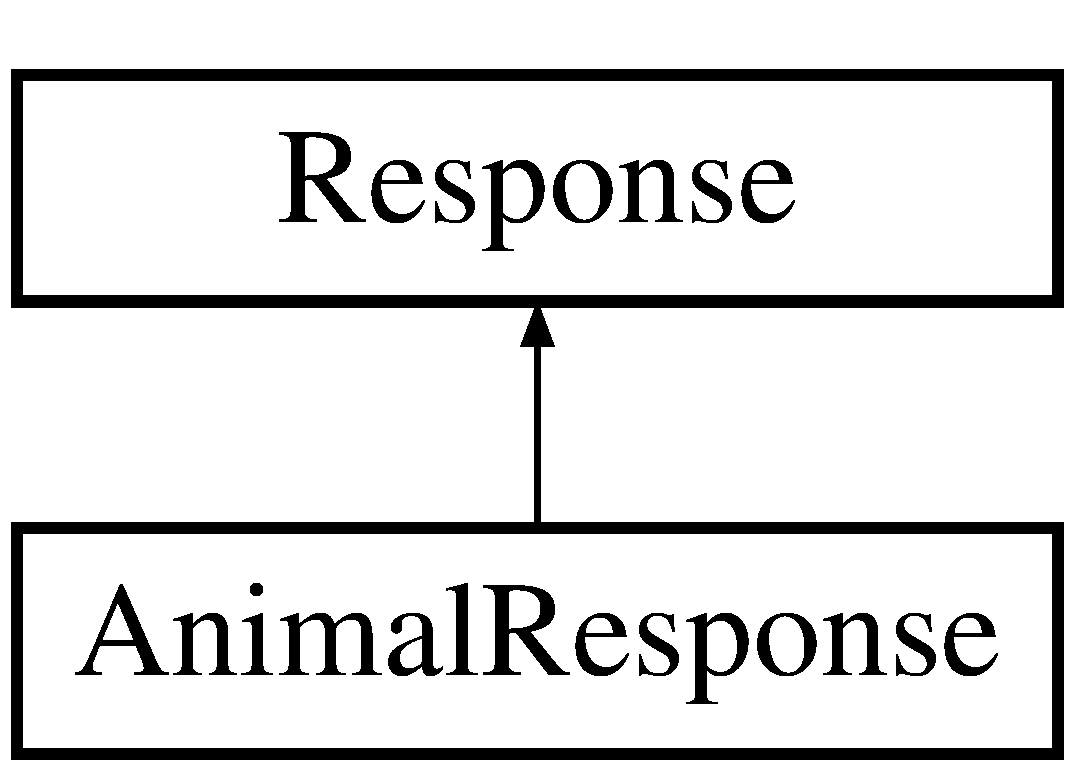
\includegraphics[height=2.000000cm]{classWildLifeTracker_1_1Response_1_1AnimalResponse}
\end{center}
\end{figure}
\subsection*{Properties}
\begin{DoxyCompactItemize}
\item 
\hyperlink{classWildLifeTracker_1_1Models_1_1Animal}{Animal} \hyperlink{classWildLifeTracker_1_1Response_1_1AnimalResponse_a364c7e4092980c5a9be7c56a2c810c18}{animal}\hspace{0.3cm}{\ttfamily  \mbox{[}get, set\mbox{]}}
\item 
List$<$ \hyperlink{classWildLifeTracker_1_1Models_1_1Animal}{Animal} $>$ \hyperlink{classWildLifeTracker_1_1Response_1_1AnimalResponse_a4c541d3fabb48f76436375ec172d1f8f}{animal\+List}\hspace{0.3cm}{\ttfamily  \mbox{[}get, set\mbox{]}}
\item 
List$<$ \hyperlink{classWildLifeTracker_1_1Models_1_1AnimalCount}{Animal\+Count} $>$ \hyperlink{classWildLifeTracker_1_1Response_1_1AnimalResponse_ae903caec3c5fee29b30564b40d89cd18}{total\+Animal\+Details}\hspace{0.3cm}{\ttfamily  \mbox{[}get, set\mbox{]}}
\end{DoxyCompactItemize}


\subsection{Detailed Description}
The model is used to create a response for animal operation 



\subsection{Property Documentation}
\mbox{\Hypertarget{classWildLifeTracker_1_1Response_1_1AnimalResponse_a364c7e4092980c5a9be7c56a2c810c18}\label{classWildLifeTracker_1_1Response_1_1AnimalResponse_a364c7e4092980c5a9be7c56a2c810c18}} 
\index{Wild\+Life\+Tracker\+::\+Response\+::\+Animal\+Response@{Wild\+Life\+Tracker\+::\+Response\+::\+Animal\+Response}!animal@{animal}}
\index{animal@{animal}!Wild\+Life\+Tracker\+::\+Response\+::\+Animal\+Response@{Wild\+Life\+Tracker\+::\+Response\+::\+Animal\+Response}}
\subsubsection{\texorpdfstring{animal}{animal}}
{\footnotesize\ttfamily \hyperlink{classWildLifeTracker_1_1Models_1_1Animal}{Animal} animal\hspace{0.3cm}{\ttfamily [get]}, {\ttfamily [set]}}

\mbox{\Hypertarget{classWildLifeTracker_1_1Response_1_1AnimalResponse_a4c541d3fabb48f76436375ec172d1f8f}\label{classWildLifeTracker_1_1Response_1_1AnimalResponse_a4c541d3fabb48f76436375ec172d1f8f}} 
\index{Wild\+Life\+Tracker\+::\+Response\+::\+Animal\+Response@{Wild\+Life\+Tracker\+::\+Response\+::\+Animal\+Response}!animal\+List@{animal\+List}}
\index{animal\+List@{animal\+List}!Wild\+Life\+Tracker\+::\+Response\+::\+Animal\+Response@{Wild\+Life\+Tracker\+::\+Response\+::\+Animal\+Response}}
\subsubsection{\texorpdfstring{animal\+List}{animalList}}
{\footnotesize\ttfamily List$<$\hyperlink{classWildLifeTracker_1_1Models_1_1Animal}{Animal}$>$ animal\+List\hspace{0.3cm}{\ttfamily [get]}, {\ttfamily [set]}}

\mbox{\Hypertarget{classWildLifeTracker_1_1Response_1_1AnimalResponse_ae903caec3c5fee29b30564b40d89cd18}\label{classWildLifeTracker_1_1Response_1_1AnimalResponse_ae903caec3c5fee29b30564b40d89cd18}} 
\index{Wild\+Life\+Tracker\+::\+Response\+::\+Animal\+Response@{Wild\+Life\+Tracker\+::\+Response\+::\+Animal\+Response}!total\+Animal\+Details@{total\+Animal\+Details}}
\index{total\+Animal\+Details@{total\+Animal\+Details}!Wild\+Life\+Tracker\+::\+Response\+::\+Animal\+Response@{Wild\+Life\+Tracker\+::\+Response\+::\+Animal\+Response}}
\subsubsection{\texorpdfstring{total\+Animal\+Details}{totalAnimalDetails}}
{\footnotesize\ttfamily List$<$\hyperlink{classWildLifeTracker_1_1Models_1_1AnimalCount}{Animal\+Count}$>$ total\+Animal\+Details\hspace{0.3cm}{\ttfamily [get]}, {\ttfamily [set]}}



The documentation for this class was generated from the following file\+:\begin{DoxyCompactItemize}
\item 
Wild\+Life\+Tracker/\+Response/\hyperlink{AnimalResponse_8cs}{Animal\+Response.\+cs}\end{DoxyCompactItemize}

\hypertarget{classWildLifeTracker_1_1Response_1_1CategoryResponse}{}\section{Category\+Response}
\label{classWildLifeTracker_1_1Response_1_1CategoryResponse}\index{Category\+Response@{Category\+Response}}


The model is used to create a response for category operation  


Inheritance diagram for Category\+Response\+:\begin{figure}[H]
\begin{center}
\leavevmode
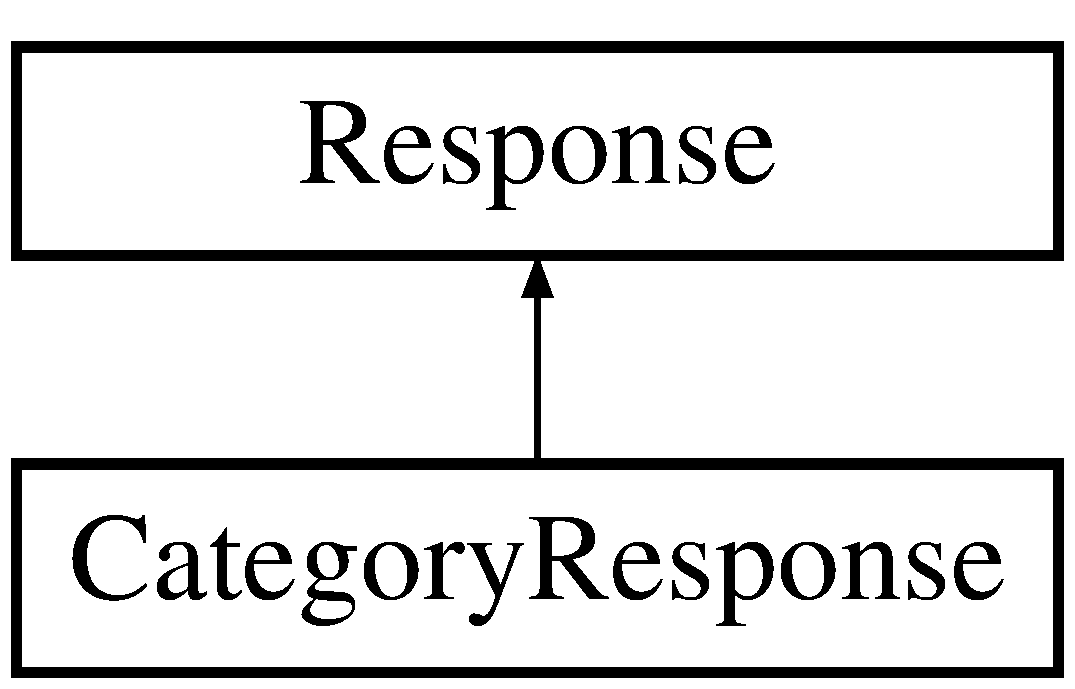
\includegraphics[height=2.000000cm]{classWildLifeTracker_1_1Response_1_1CategoryResponse}
\end{center}
\end{figure}
\subsection*{Properties}
\begin{DoxyCompactItemize}
\item 
\hyperlink{classWildLifeTracker_1_1Models_1_1Category}{Category} \hyperlink{classWildLifeTracker_1_1Response_1_1CategoryResponse_a08b424ccd4f519f4a97826f9d3f3f094}{category}\hspace{0.3cm}{\ttfamily  \mbox{[}get, set\mbox{]}}
\item 
List$<$ \hyperlink{classWildLifeTracker_1_1Models_1_1Category}{Category} $>$ \hyperlink{classWildLifeTracker_1_1Response_1_1CategoryResponse_ac20f04846190de6a34eadd21501afae3}{category\+List}\hspace{0.3cm}{\ttfamily  \mbox{[}get, set\mbox{]}}
\end{DoxyCompactItemize}


\subsection{Detailed Description}
The model is used to create a response for category operation 



\subsection{Property Documentation}
\mbox{\Hypertarget{classWildLifeTracker_1_1Response_1_1CategoryResponse_a08b424ccd4f519f4a97826f9d3f3f094}\label{classWildLifeTracker_1_1Response_1_1CategoryResponse_a08b424ccd4f519f4a97826f9d3f3f094}} 
\index{Wild\+Life\+Tracker\+::\+Response\+::\+Category\+Response@{Wild\+Life\+Tracker\+::\+Response\+::\+Category\+Response}!category@{category}}
\index{category@{category}!Wild\+Life\+Tracker\+::\+Response\+::\+Category\+Response@{Wild\+Life\+Tracker\+::\+Response\+::\+Category\+Response}}
\subsubsection{\texorpdfstring{category}{category}}
{\footnotesize\ttfamily \hyperlink{classWildLifeTracker_1_1Models_1_1Category}{Category} category\hspace{0.3cm}{\ttfamily [get]}, {\ttfamily [set]}}

\mbox{\Hypertarget{classWildLifeTracker_1_1Response_1_1CategoryResponse_ac20f04846190de6a34eadd21501afae3}\label{classWildLifeTracker_1_1Response_1_1CategoryResponse_ac20f04846190de6a34eadd21501afae3}} 
\index{Wild\+Life\+Tracker\+::\+Response\+::\+Category\+Response@{Wild\+Life\+Tracker\+::\+Response\+::\+Category\+Response}!category\+List@{category\+List}}
\index{category\+List@{category\+List}!Wild\+Life\+Tracker\+::\+Response\+::\+Category\+Response@{Wild\+Life\+Tracker\+::\+Response\+::\+Category\+Response}}
\subsubsection{\texorpdfstring{category\+List}{categoryList}}
{\footnotesize\ttfamily List$<$\hyperlink{classWildLifeTracker_1_1Models_1_1Category}{Category}$>$ category\+List\hspace{0.3cm}{\ttfamily [get]}, {\ttfamily [set]}}



The documentation for this class was generated from the following file\+:\begin{DoxyCompactItemize}
\item 
Wild\+Life\+Tracker/\+Response/\hyperlink{CategoryResponse_8cs}{Category\+Response.\+cs}\end{DoxyCompactItemize}

\hypertarget{classWildLifeTracker_1_1Response_1_1Response}{}\section{Response}
\label{classWildLifeTracker_1_1Response_1_1Response}\index{Response@{Response}}
Inheritance diagram for Response\+:\begin{figure}[H]
\begin{center}
\leavevmode
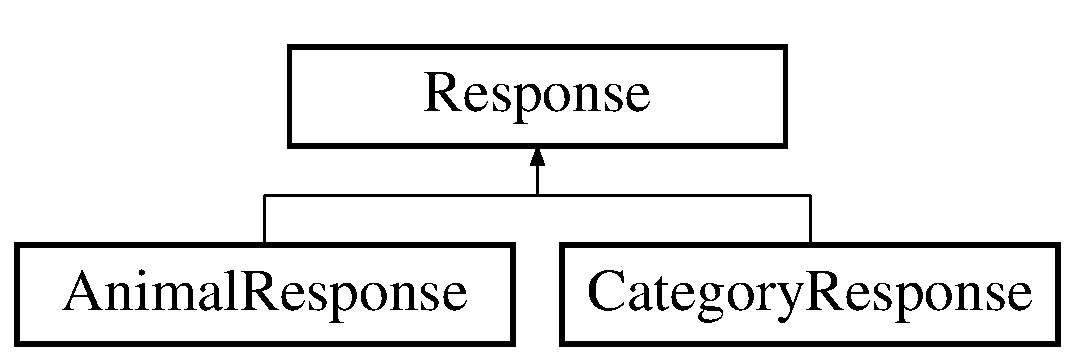
\includegraphics[height=2.000000cm]{classWildLifeTracker_1_1Response_1_1Response}
\end{center}
\end{figure}
\subsection*{Properties}
\begin{DoxyCompactItemize}
\item 
string \hyperlink{classWildLifeTracker_1_1Response_1_1Response_ae1ed0d7a6f352c7ee3ad978429822c6f}{message}\hspace{0.3cm}{\ttfamily  \mbox{[}get, set\mbox{]}}
\begin{DoxyCompactList}\small\item\em The model is used to send any messages if needed. \end{DoxyCompactList}\end{DoxyCompactItemize}


\subsection{Property Documentation}
\mbox{\Hypertarget{classWildLifeTracker_1_1Response_1_1Response_ae1ed0d7a6f352c7ee3ad978429822c6f}\label{classWildLifeTracker_1_1Response_1_1Response_ae1ed0d7a6f352c7ee3ad978429822c6f}} 
\index{Wild\+Life\+Tracker\+::\+Response\+::\+Response@{Wild\+Life\+Tracker\+::\+Response\+::\+Response}!message@{message}}
\index{message@{message}!Wild\+Life\+Tracker\+::\+Response\+::\+Response@{Wild\+Life\+Tracker\+::\+Response\+::\+Response}}
\subsubsection{\texorpdfstring{message}{message}}
{\footnotesize\ttfamily string message\hspace{0.3cm}{\ttfamily [get]}, {\ttfamily [set]}}



The model is used to send any messages if needed. 



The documentation for this class was generated from the following file\+:\begin{DoxyCompactItemize}
\item 
Wild\+Life\+Tracker/\+Response/\hyperlink{Response_8cs}{Response.\+cs}\end{DoxyCompactItemize}

\hypertarget{classWildLifeTracker_1_1Response_1_1TrackingInfoResponse}{}\section{Tracking\+Info\+Response}
\label{classWildLifeTracker_1_1Response_1_1TrackingInfoResponse}\index{Tracking\+Info\+Response@{Tracking\+Info\+Response}}


The model is used to create a response for tracking operation  


\subsection*{Properties}
\begin{DoxyCompactItemize}
\item 
List$<$ \hyperlink{classWildLifeTracker_1_1Models_1_1GPSTrackingInfo}{G\+P\+S\+Tracking\+Info} $>$ \hyperlink{classWildLifeTracker_1_1Response_1_1TrackingInfoResponse_a10d74e08741c172f7ae042149bf3147c}{gps\+Tracking\+Details}\hspace{0.3cm}{\ttfamily  \mbox{[}get, set\mbox{]}}
\end{DoxyCompactItemize}


\subsection{Detailed Description}
The model is used to create a response for tracking operation 



\subsection{Property Documentation}
\mbox{\Hypertarget{classWildLifeTracker_1_1Response_1_1TrackingInfoResponse_a10d74e08741c172f7ae042149bf3147c}\label{classWildLifeTracker_1_1Response_1_1TrackingInfoResponse_a10d74e08741c172f7ae042149bf3147c}} 
\index{Wild\+Life\+Tracker\+::\+Response\+::\+Tracking\+Info\+Response@{Wild\+Life\+Tracker\+::\+Response\+::\+Tracking\+Info\+Response}!gps\+Tracking\+Details@{gps\+Tracking\+Details}}
\index{gps\+Tracking\+Details@{gps\+Tracking\+Details}!Wild\+Life\+Tracker\+::\+Response\+::\+Tracking\+Info\+Response@{Wild\+Life\+Tracker\+::\+Response\+::\+Tracking\+Info\+Response}}
\subsubsection{\texorpdfstring{gps\+Tracking\+Details}{gpsTrackingDetails}}
{\footnotesize\ttfamily List$<$\hyperlink{classWildLifeTracker_1_1Models_1_1GPSTrackingInfo}{G\+P\+S\+Tracking\+Info}$>$ gps\+Tracking\+Details\hspace{0.3cm}{\ttfamily [get]}, {\ttfamily [set]}}



The documentation for this class was generated from the following file\+:\begin{DoxyCompactItemize}
\item 
Wild\+Life\+Tracker/\+Response/\hyperlink{TrackingInfoResponse_8cs}{Tracking\+Info\+Response.\+cs}\end{DoxyCompactItemize}

\hypertarget{classWildLifeTracker_1_1Services_1_1AnimalService}{}\section{Animal\+Service}
\label{classWildLifeTracker_1_1Services_1_1AnimalService}\index{Animal\+Service@{Animal\+Service}}


Animal Service to perform different operations.  


Inheritance diagram for Animal\+Service\+:\begin{figure}[H]
\begin{center}
\leavevmode
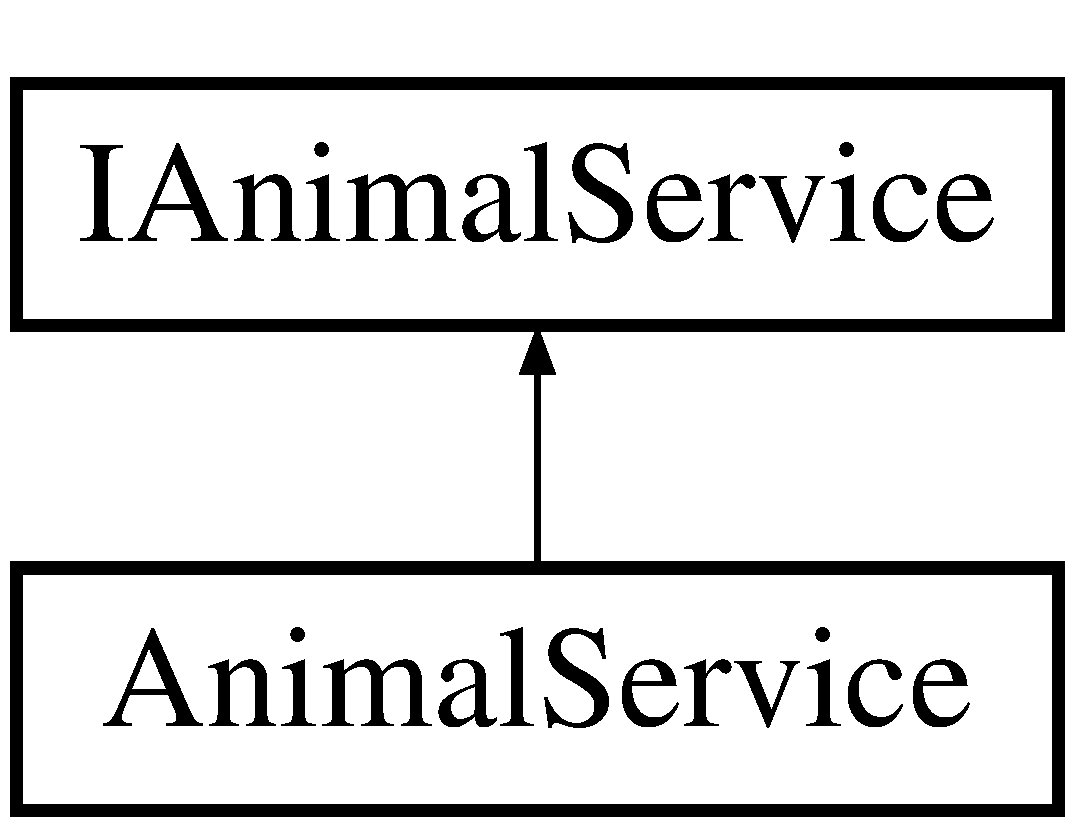
\includegraphics[height=2.000000cm]{classWildLifeTracker_1_1Services_1_1AnimalService}
\end{center}
\end{figure}
\subsection*{Public Member Functions}
\begin{DoxyCompactItemize}
\item 
\hyperlink{classWildLifeTracker_1_1Services_1_1AnimalService_aec71da8266bf866afd3e09fa74e2bf6b}{Animal\+Service} ()
\begin{DoxyCompactList}\small\item\em Constructor that intialize log4net in class \end{DoxyCompactList}\item 
\hyperlink{classWildLifeTracker_1_1Response_1_1AnimalResponse}{Animal\+Response} \hyperlink{classWildLifeTracker_1_1Services_1_1AnimalService_ae578d708ed9407d8805d69b193eff67b}{Add\+Animal} (\hyperlink{classWildLifeTracker_1_1Models_1_1Animal}{Animal} animal\+Details)
\begin{DoxyCompactList}\small\item\em Add the animals to the G\+PS device \end{DoxyCompactList}\item 
\hyperlink{classWildLifeTracker_1_1Response_1_1AnimalResponse}{Animal\+Response} \hyperlink{classWildLifeTracker_1_1Services_1_1AnimalService_a201e384747e50bd19c431955eae072fa}{Delete\+Animal} (string animal\+Id)
\begin{DoxyCompactList}\small\item\em Deletes the animals \end{DoxyCompactList}\item 
\hyperlink{classWildLifeTracker_1_1Response_1_1AnimalResponse}{Animal\+Response} \hyperlink{classWildLifeTracker_1_1Services_1_1AnimalService_a38b8ef318dc92ac93cfcbbc33a454c5a}{Get\+All\+Animals} ()
\begin{DoxyCompactList}\small\item\em Retrieves all the animals \end{DoxyCompactList}\item 
\hyperlink{classWildLifeTracker_1_1Response_1_1AnimalResponse}{Animal\+Response} \hyperlink{classWildLifeTracker_1_1Services_1_1AnimalService_aa4dc53f849ee7b88879fa17f9d48bd42}{Get\+Animals\+Count\+Per\+Category} (string from\+Date, string to\+Date)
\begin{DoxyCompactList}\small\item\em Retrieves the animal details per category \end{DoxyCompactList}\item 
\hyperlink{classWildLifeTracker_1_1Response_1_1AnimalResponse}{Animal\+Response} \hyperlink{classWildLifeTracker_1_1Services_1_1AnimalService_a4b971311981c685104e1b3403c87372a}{Get\+Animals\+Percategory} (string categor\+Id)
\begin{DoxyCompactList}\small\item\em Retrieves the animals per category \end{DoxyCompactList}\item 
\hyperlink{classWildLifeTracker_1_1Response_1_1AnimalResponse}{Animal\+Response} \hyperlink{classWildLifeTracker_1_1Services_1_1AnimalService_a993d3155da89897e5403799432be158b}{Update\+Animal} (\hyperlink{classWildLifeTracker_1_1Models_1_1Animal}{Animal} animal\+Details)
\begin{DoxyCompactList}\small\item\em Updates an animal details \end{DoxyCompactList}\end{DoxyCompactItemize}
\subsection*{Properties}
\begin{DoxyCompactItemize}
\item 
static log4net.\+I\+Log \hyperlink{classWildLifeTracker_1_1Services_1_1AnimalService_a5fc9abb86e6110ecd61d0a1a7d740a8a}{Log}\hspace{0.3cm}{\ttfamily  \mbox{[}get, private set\mbox{]}}
\end{DoxyCompactItemize}
\subsection*{Private Attributes}
\begin{DoxyCompactItemize}
\item 
\hyperlink{classWildLifeTracker_1_1Repository_1_1AnimalRepo}{Animal\+Repo} \hyperlink{classWildLifeTracker_1_1Services_1_1AnimalService_aead7289ee5f2ad9a13ff6b43698a76bb}{animal\+Repo} = null
\end{DoxyCompactItemize}
\subsection*{Static Private Attributes}
\begin{DoxyCompactItemize}
\item 
static readonly log4net.\+I\+Log \hyperlink{classWildLifeTracker_1_1Services_1_1AnimalService_ae6c6142b8525b2f4ac6ee6e003b3106f}{log}
\end{DoxyCompactItemize}


\subsection{Detailed Description}
Animal Service to perform different operations. 



\subsection{Constructor \& Destructor Documentation}
\mbox{\Hypertarget{classWildLifeTracker_1_1Services_1_1AnimalService_aec71da8266bf866afd3e09fa74e2bf6b}\label{classWildLifeTracker_1_1Services_1_1AnimalService_aec71da8266bf866afd3e09fa74e2bf6b}} 
\index{Wild\+Life\+Tracker\+::\+Services\+::\+Animal\+Service@{Wild\+Life\+Tracker\+::\+Services\+::\+Animal\+Service}!Animal\+Service@{Animal\+Service}}
\index{Animal\+Service@{Animal\+Service}!Wild\+Life\+Tracker\+::\+Services\+::\+Animal\+Service@{Wild\+Life\+Tracker\+::\+Services\+::\+Animal\+Service}}
\subsubsection{\texorpdfstring{Animal\+Service()}{AnimalService()}}
{\footnotesize\ttfamily \hyperlink{classWildLifeTracker_1_1Services_1_1AnimalService}{Animal\+Service} (\begin{DoxyParamCaption}{ }\end{DoxyParamCaption})\hspace{0.3cm}{\ttfamily [inline]}}



Constructor that intialize log4net in class 



\subsection{Member Function Documentation}
\mbox{\Hypertarget{classWildLifeTracker_1_1Services_1_1AnimalService_ae578d708ed9407d8805d69b193eff67b}\label{classWildLifeTracker_1_1Services_1_1AnimalService_ae578d708ed9407d8805d69b193eff67b}} 
\index{Wild\+Life\+Tracker\+::\+Services\+::\+Animal\+Service@{Wild\+Life\+Tracker\+::\+Services\+::\+Animal\+Service}!Add\+Animal@{Add\+Animal}}
\index{Add\+Animal@{Add\+Animal}!Wild\+Life\+Tracker\+::\+Services\+::\+Animal\+Service@{Wild\+Life\+Tracker\+::\+Services\+::\+Animal\+Service}}
\subsubsection{\texorpdfstring{Add\+Animal()}{AddAnimal()}}
{\footnotesize\ttfamily \hyperlink{classWildLifeTracker_1_1Response_1_1AnimalResponse}{Animal\+Response} Add\+Animal (\begin{DoxyParamCaption}\item[{\hyperlink{classWildLifeTracker_1_1Models_1_1Animal}{Animal}}]{animal\+Details }\end{DoxyParamCaption})\hspace{0.3cm}{\ttfamily [inline]}}



Add the animals to the G\+PS device 


\begin{DoxyParams}{Parameters}
{\em animal\+Details} & The animal details\\
\hline
\end{DoxyParams}
\begin{DoxyReturn}{Returns}
The details of animal that is added
\end{DoxyReturn}


Implements \hyperlink{interfaceWildLifeTracker_1_1Services_1_1IAnimalService_ae578d708ed9407d8805d69b193eff67b}{I\+Animal\+Service}.

\mbox{\Hypertarget{classWildLifeTracker_1_1Services_1_1AnimalService_a201e384747e50bd19c431955eae072fa}\label{classWildLifeTracker_1_1Services_1_1AnimalService_a201e384747e50bd19c431955eae072fa}} 
\index{Wild\+Life\+Tracker\+::\+Services\+::\+Animal\+Service@{Wild\+Life\+Tracker\+::\+Services\+::\+Animal\+Service}!Delete\+Animal@{Delete\+Animal}}
\index{Delete\+Animal@{Delete\+Animal}!Wild\+Life\+Tracker\+::\+Services\+::\+Animal\+Service@{Wild\+Life\+Tracker\+::\+Services\+::\+Animal\+Service}}
\subsubsection{\texorpdfstring{Delete\+Animal()}{DeleteAnimal()}}
{\footnotesize\ttfamily \hyperlink{classWildLifeTracker_1_1Response_1_1AnimalResponse}{Animal\+Response} Delete\+Animal (\begin{DoxyParamCaption}\item[{string}]{animal\+Id }\end{DoxyParamCaption})\hspace{0.3cm}{\ttfamily [inline]}}



Deletes the animals 


\begin{DoxyParams}{Parameters}
{\em animal\+Id} & The animal id\\
\hline
\end{DoxyParams}
\begin{DoxyReturn}{Returns}
Details of animals
\end{DoxyReturn}


Implements \hyperlink{interfaceWildLifeTracker_1_1Services_1_1IAnimalService_a201e384747e50bd19c431955eae072fa}{I\+Animal\+Service}.

\mbox{\Hypertarget{classWildLifeTracker_1_1Services_1_1AnimalService_a38b8ef318dc92ac93cfcbbc33a454c5a}\label{classWildLifeTracker_1_1Services_1_1AnimalService_a38b8ef318dc92ac93cfcbbc33a454c5a}} 
\index{Wild\+Life\+Tracker\+::\+Services\+::\+Animal\+Service@{Wild\+Life\+Tracker\+::\+Services\+::\+Animal\+Service}!Get\+All\+Animals@{Get\+All\+Animals}}
\index{Get\+All\+Animals@{Get\+All\+Animals}!Wild\+Life\+Tracker\+::\+Services\+::\+Animal\+Service@{Wild\+Life\+Tracker\+::\+Services\+::\+Animal\+Service}}
\subsubsection{\texorpdfstring{Get\+All\+Animals()}{GetAllAnimals()}}
{\footnotesize\ttfamily \hyperlink{classWildLifeTracker_1_1Response_1_1AnimalResponse}{Animal\+Response} Get\+All\+Animals (\begin{DoxyParamCaption}{ }\end{DoxyParamCaption})\hspace{0.3cm}{\ttfamily [inline]}}



Retrieves all the animals 

\begin{DoxyReturn}{Returns}
All the animals
\end{DoxyReturn}


Implements \hyperlink{interfaceWildLifeTracker_1_1Services_1_1IAnimalService_a38b8ef318dc92ac93cfcbbc33a454c5a}{I\+Animal\+Service}.

\mbox{\Hypertarget{classWildLifeTracker_1_1Services_1_1AnimalService_aa4dc53f849ee7b88879fa17f9d48bd42}\label{classWildLifeTracker_1_1Services_1_1AnimalService_aa4dc53f849ee7b88879fa17f9d48bd42}} 
\index{Wild\+Life\+Tracker\+::\+Services\+::\+Animal\+Service@{Wild\+Life\+Tracker\+::\+Services\+::\+Animal\+Service}!Get\+Animals\+Count\+Per\+Category@{Get\+Animals\+Count\+Per\+Category}}
\index{Get\+Animals\+Count\+Per\+Category@{Get\+Animals\+Count\+Per\+Category}!Wild\+Life\+Tracker\+::\+Services\+::\+Animal\+Service@{Wild\+Life\+Tracker\+::\+Services\+::\+Animal\+Service}}
\subsubsection{\texorpdfstring{Get\+Animals\+Count\+Per\+Category()}{GetAnimalsCountPerCategory()}}
{\footnotesize\ttfamily \hyperlink{classWildLifeTracker_1_1Response_1_1AnimalResponse}{Animal\+Response} Get\+Animals\+Count\+Per\+Category (\begin{DoxyParamCaption}\item[{string}]{from\+Date,  }\item[{string}]{to\+Date }\end{DoxyParamCaption})\hspace{0.3cm}{\ttfamily [inline]}}



Retrieves the animal details per category 


\begin{DoxyParams}{Parameters}
{\em from\+Date} & The from date\\
\hline
{\em to\+Date} & The end date\\
\hline
\end{DoxyParams}
\begin{DoxyReturn}{Returns}
Details of count of animals per category over the duration
\end{DoxyReturn}


Implements \hyperlink{interfaceWildLifeTracker_1_1Services_1_1IAnimalService_aa4dc53f849ee7b88879fa17f9d48bd42}{I\+Animal\+Service}.

\mbox{\Hypertarget{classWildLifeTracker_1_1Services_1_1AnimalService_a4b971311981c685104e1b3403c87372a}\label{classWildLifeTracker_1_1Services_1_1AnimalService_a4b971311981c685104e1b3403c87372a}} 
\index{Wild\+Life\+Tracker\+::\+Services\+::\+Animal\+Service@{Wild\+Life\+Tracker\+::\+Services\+::\+Animal\+Service}!Get\+Animals\+Percategory@{Get\+Animals\+Percategory}}
\index{Get\+Animals\+Percategory@{Get\+Animals\+Percategory}!Wild\+Life\+Tracker\+::\+Services\+::\+Animal\+Service@{Wild\+Life\+Tracker\+::\+Services\+::\+Animal\+Service}}
\subsubsection{\texorpdfstring{Get\+Animals\+Percategory()}{GetAnimalsPercategory()}}
{\footnotesize\ttfamily \hyperlink{classWildLifeTracker_1_1Response_1_1AnimalResponse}{Animal\+Response} Get\+Animals\+Percategory (\begin{DoxyParamCaption}\item[{string}]{categor\+Id }\end{DoxyParamCaption})\hspace{0.3cm}{\ttfamily [inline]}}



Retrieves the animals per category 


\begin{DoxyParams}{Parameters}
{\em categor\+Id} & The category\+Id\\
\hline
\end{DoxyParams}
\begin{DoxyReturn}{Returns}
Details of animals per category
\end{DoxyReturn}


Implements \hyperlink{interfaceWildLifeTracker_1_1Services_1_1IAnimalService_aa701643cef16849a06696c926b87d46d}{I\+Animal\+Service}.

\mbox{\Hypertarget{classWildLifeTracker_1_1Services_1_1AnimalService_a993d3155da89897e5403799432be158b}\label{classWildLifeTracker_1_1Services_1_1AnimalService_a993d3155da89897e5403799432be158b}} 
\index{Wild\+Life\+Tracker\+::\+Services\+::\+Animal\+Service@{Wild\+Life\+Tracker\+::\+Services\+::\+Animal\+Service}!Update\+Animal@{Update\+Animal}}
\index{Update\+Animal@{Update\+Animal}!Wild\+Life\+Tracker\+::\+Services\+::\+Animal\+Service@{Wild\+Life\+Tracker\+::\+Services\+::\+Animal\+Service}}
\subsubsection{\texorpdfstring{Update\+Animal()}{UpdateAnimal()}}
{\footnotesize\ttfamily \hyperlink{classWildLifeTracker_1_1Response_1_1AnimalResponse}{Animal\+Response} Update\+Animal (\begin{DoxyParamCaption}\item[{\hyperlink{classWildLifeTracker_1_1Models_1_1Animal}{Animal}}]{animal\+Details }\end{DoxyParamCaption})\hspace{0.3cm}{\ttfamily [inline]}}



Updates an animal details 


\begin{DoxyParams}{Parameters}
{\em animal\+Details} & The animal details\\
\hline
\end{DoxyParams}
\begin{DoxyReturn}{Returns}
Details of updated animal
\end{DoxyReturn}


Implements \hyperlink{interfaceWildLifeTracker_1_1Services_1_1IAnimalService_a993d3155da89897e5403799432be158b}{I\+Animal\+Service}.



\subsection{Member Data Documentation}
\mbox{\Hypertarget{classWildLifeTracker_1_1Services_1_1AnimalService_aead7289ee5f2ad9a13ff6b43698a76bb}\label{classWildLifeTracker_1_1Services_1_1AnimalService_aead7289ee5f2ad9a13ff6b43698a76bb}} 
\index{Wild\+Life\+Tracker\+::\+Services\+::\+Animal\+Service@{Wild\+Life\+Tracker\+::\+Services\+::\+Animal\+Service}!animal\+Repo@{animal\+Repo}}
\index{animal\+Repo@{animal\+Repo}!Wild\+Life\+Tracker\+::\+Services\+::\+Animal\+Service@{Wild\+Life\+Tracker\+::\+Services\+::\+Animal\+Service}}
\subsubsection{\texorpdfstring{animal\+Repo}{animalRepo}}
{\footnotesize\ttfamily \hyperlink{classWildLifeTracker_1_1Repository_1_1AnimalRepo}{Animal\+Repo} animal\+Repo = null\hspace{0.3cm}{\ttfamily [private]}}

\mbox{\Hypertarget{classWildLifeTracker_1_1Services_1_1AnimalService_ae6c6142b8525b2f4ac6ee6e003b3106f}\label{classWildLifeTracker_1_1Services_1_1AnimalService_ae6c6142b8525b2f4ac6ee6e003b3106f}} 
\index{Wild\+Life\+Tracker\+::\+Services\+::\+Animal\+Service@{Wild\+Life\+Tracker\+::\+Services\+::\+Animal\+Service}!log@{log}}
\index{log@{log}!Wild\+Life\+Tracker\+::\+Services\+::\+Animal\+Service@{Wild\+Life\+Tracker\+::\+Services\+::\+Animal\+Service}}
\subsubsection{\texorpdfstring{log}{log}}
{\footnotesize\ttfamily readonly log4net.\+I\+Log log\hspace{0.3cm}{\ttfamily [static]}, {\ttfamily [private]}}

{\bfseries Initial value\+:}
\begin{DoxyCode}
= log4net.LogManager.GetLogger
       (\hyperlink{namespaceSystem}{System}.Reflection.MethodBase.GetCurrentMethod().DeclaringType)
\end{DoxyCode}


\subsection{Property Documentation}
\mbox{\Hypertarget{classWildLifeTracker_1_1Services_1_1AnimalService_a5fc9abb86e6110ecd61d0a1a7d740a8a}\label{classWildLifeTracker_1_1Services_1_1AnimalService_a5fc9abb86e6110ecd61d0a1a7d740a8a}} 
\index{Wild\+Life\+Tracker\+::\+Services\+::\+Animal\+Service@{Wild\+Life\+Tracker\+::\+Services\+::\+Animal\+Service}!Log@{Log}}
\index{Log@{Log}!Wild\+Life\+Tracker\+::\+Services\+::\+Animal\+Service@{Wild\+Life\+Tracker\+::\+Services\+::\+Animal\+Service}}
\subsubsection{\texorpdfstring{Log}{Log}}
{\footnotesize\ttfamily log4net.\+I\+Log Log\hspace{0.3cm}{\ttfamily [static]}, {\ttfamily [get]}, {\ttfamily [private set]}}



The documentation for this class was generated from the following file\+:\begin{DoxyCompactItemize}
\item 
Wild\+Life\+Tracker/\+Services/\hyperlink{AnimalService_8svc_8cs}{Animal\+Service.\+svc.\+cs}\end{DoxyCompactItemize}

\hypertarget{interfaceWildLifeTracker_1_1Services_1_1IAnimalService}{}\section{I\+Animal\+Service}
\label{interfaceWildLifeTracker_1_1Services_1_1IAnimalService}\index{I\+Animal\+Service@{I\+Animal\+Service}}


The interface exposes all the A\+P\+Is for animal details  


Inheritance diagram for I\+Animal\+Service\+:\begin{figure}[H]
\begin{center}
\leavevmode
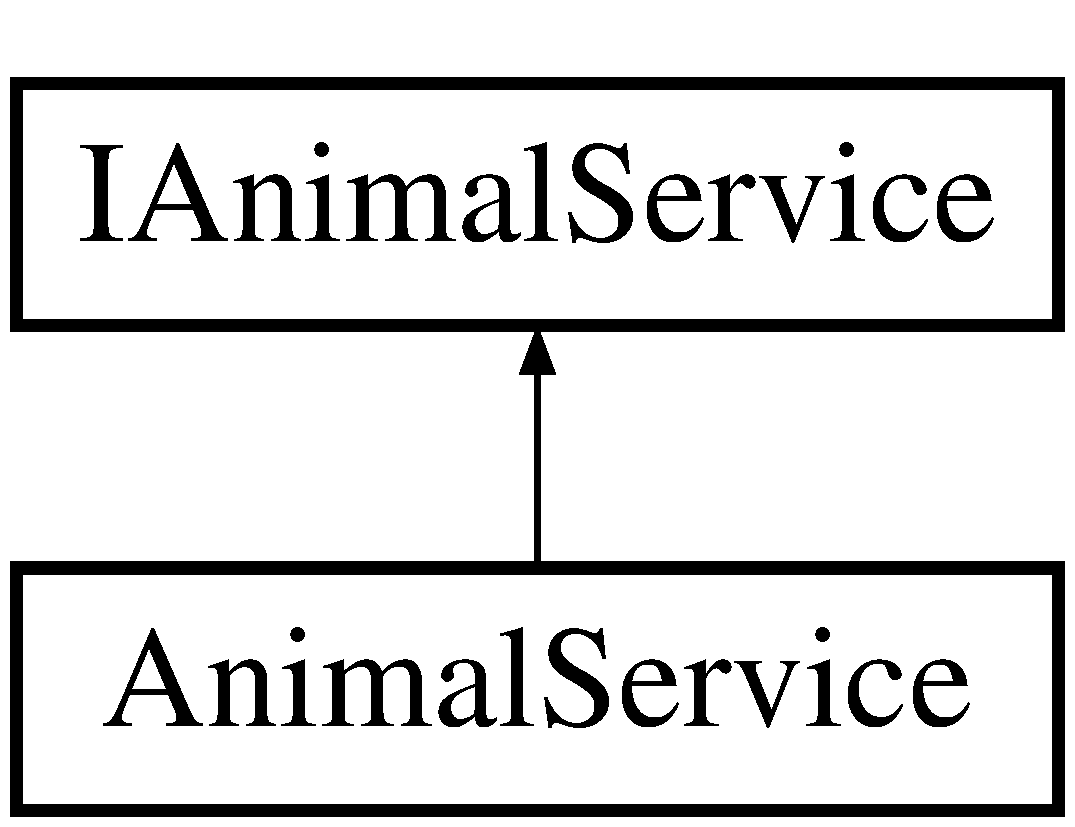
\includegraphics[height=2.000000cm]{interfaceWildLifeTracker_1_1Services_1_1IAnimalService}
\end{center}
\end{figure}
\subsection*{Public Member Functions}
\begin{DoxyCompactItemize}
\item 
\hyperlink{classWildLifeTracker_1_1Response_1_1AnimalResponse}{Animal\+Response} \hyperlink{interfaceWildLifeTracker_1_1Services_1_1IAnimalService_ae578d708ed9407d8805d69b193eff67b}{Add\+Animal} (\hyperlink{classWildLifeTracker_1_1Models_1_1Animal}{Animal} animal\+Details)
\begin{DoxyCompactList}\small\item\em Adds a new animal. 
\begin{DoxyParams}{Parameters}
{\em animal\+Details} & The animal details to be added\\
\hline
\end{DoxyParams}
\begin{DoxyReturn}{Returns}
Returns the animal details for the newly created animal or throws Exception
\end{DoxyReturn}
\end{DoxyCompactList}\item 
\hyperlink{classWildLifeTracker_1_1Response_1_1AnimalResponse}{Animal\+Response} \hyperlink{interfaceWildLifeTracker_1_1Services_1_1IAnimalService_a201e384747e50bd19c431955eae072fa}{Delete\+Animal} (string animal\+Id)
\begin{DoxyCompactList}\small\item\em Delete the animal details. 
\begin{DoxyParams}{Parameters}
{\em animal\+Id} & the animal id\\
\hline
\end{DoxyParams}
\begin{DoxyReturn}{Returns}
Returns the animal details of animal that is deleted
\end{DoxyReturn}
\end{DoxyCompactList}\item 
\hyperlink{classWildLifeTracker_1_1Response_1_1AnimalResponse}{Animal\+Response} \hyperlink{interfaceWildLifeTracker_1_1Services_1_1IAnimalService_a38b8ef318dc92ac93cfcbbc33a454c5a}{Get\+All\+Animals} ()
\begin{DoxyCompactList}\small\item\em Retrieves all the animals \begin{DoxyReturn}{Returns}
Returns all the animal details
\end{DoxyReturn}
\end{DoxyCompactList}\item 
\hyperlink{classWildLifeTracker_1_1Response_1_1AnimalResponse}{Animal\+Response} \hyperlink{interfaceWildLifeTracker_1_1Services_1_1IAnimalService_aa4dc53f849ee7b88879fa17f9d48bd42}{Get\+Animals\+Count\+Per\+Category} (string from\+Date, string to\+Date)
\begin{DoxyCompactList}\small\item\em Update an animal details. 
\begin{DoxyParams}{Parameters}
{\em from\+Date} & from date\\
\hline
{\em to\+Date} & to date\\
\hline
\end{DoxyParams}
\begin{DoxyReturn}{Returns}
Returns the count of animal per category
\end{DoxyReturn}
\end{DoxyCompactList}\item 
\hyperlink{classWildLifeTracker_1_1Response_1_1AnimalResponse}{Animal\+Response} \hyperlink{interfaceWildLifeTracker_1_1Services_1_1IAnimalService_aa701643cef16849a06696c926b87d46d}{Get\+Animals\+Percategory} (string category\+Id)
\begin{DoxyCompactList}\small\item\em Retrieves all the animal when category\+Id is specified. 
\begin{DoxyParams}{Parameters}
{\em category\+Id} & the category id\\
\hline
\end{DoxyParams}
\begin{DoxyReturn}{Returns}
Returns animal per category
\end{DoxyReturn}
\end{DoxyCompactList}\item 
\hyperlink{classWildLifeTracker_1_1Response_1_1AnimalResponse}{Animal\+Response} \hyperlink{interfaceWildLifeTracker_1_1Services_1_1IAnimalService_a993d3155da89897e5403799432be158b}{Update\+Animal} (\hyperlink{classWildLifeTracker_1_1Models_1_1Animal}{Animal} animal\+Details)
\begin{DoxyCompactList}\small\item\em Update an animal details. 
\begin{DoxyParams}{Parameters}
{\em animal\+Details} & the animal details\\
\hline
\end{DoxyParams}
\begin{DoxyReturn}{Returns}
Returns the animal details of updated animal
\end{DoxyReturn}
\end{DoxyCompactList}\end{DoxyCompactItemize}


\subsection{Detailed Description}
The interface exposes all the A\+P\+Is for animal details 



\subsection{Member Function Documentation}
\mbox{\Hypertarget{interfaceWildLifeTracker_1_1Services_1_1IAnimalService_ae578d708ed9407d8805d69b193eff67b}\label{interfaceWildLifeTracker_1_1Services_1_1IAnimalService_ae578d708ed9407d8805d69b193eff67b}} 
\index{Wild\+Life\+Tracker\+::\+Services\+::\+I\+Animal\+Service@{Wild\+Life\+Tracker\+::\+Services\+::\+I\+Animal\+Service}!Add\+Animal@{Add\+Animal}}
\index{Add\+Animal@{Add\+Animal}!Wild\+Life\+Tracker\+::\+Services\+::\+I\+Animal\+Service@{Wild\+Life\+Tracker\+::\+Services\+::\+I\+Animal\+Service}}
\subsubsection{\texorpdfstring{Add\+Animal()}{AddAnimal()}}
{\footnotesize\ttfamily \hyperlink{classWildLifeTracker_1_1Response_1_1AnimalResponse}{Animal\+Response} Add\+Animal (\begin{DoxyParamCaption}\item[{\hyperlink{classWildLifeTracker_1_1Models_1_1Animal}{Animal}}]{animal\+Details }\end{DoxyParamCaption})}



Adds a new animal. 
\begin{DoxyParams}{Parameters}
{\em animal\+Details} & The animal details to be added\\
\hline
\end{DoxyParams}
\begin{DoxyReturn}{Returns}
Returns the animal details for the newly created animal or throws Exception
\end{DoxyReturn}




Implemented in \hyperlink{classWildLifeTracker_1_1Services_1_1AnimalService_ae578d708ed9407d8805d69b193eff67b}{Animal\+Service}.

\mbox{\Hypertarget{interfaceWildLifeTracker_1_1Services_1_1IAnimalService_a201e384747e50bd19c431955eae072fa}\label{interfaceWildLifeTracker_1_1Services_1_1IAnimalService_a201e384747e50bd19c431955eae072fa}} 
\index{Wild\+Life\+Tracker\+::\+Services\+::\+I\+Animal\+Service@{Wild\+Life\+Tracker\+::\+Services\+::\+I\+Animal\+Service}!Delete\+Animal@{Delete\+Animal}}
\index{Delete\+Animal@{Delete\+Animal}!Wild\+Life\+Tracker\+::\+Services\+::\+I\+Animal\+Service@{Wild\+Life\+Tracker\+::\+Services\+::\+I\+Animal\+Service}}
\subsubsection{\texorpdfstring{Delete\+Animal()}{DeleteAnimal()}}
{\footnotesize\ttfamily \hyperlink{classWildLifeTracker_1_1Response_1_1AnimalResponse}{Animal\+Response} Delete\+Animal (\begin{DoxyParamCaption}\item[{string}]{animal\+Id }\end{DoxyParamCaption})}



Delete the animal details. 
\begin{DoxyParams}{Parameters}
{\em animal\+Id} & the animal id\\
\hline
\end{DoxyParams}
\begin{DoxyReturn}{Returns}
Returns the animal details of animal that is deleted
\end{DoxyReturn}




Implemented in \hyperlink{classWildLifeTracker_1_1Services_1_1AnimalService_a201e384747e50bd19c431955eae072fa}{Animal\+Service}.

\mbox{\Hypertarget{interfaceWildLifeTracker_1_1Services_1_1IAnimalService_a38b8ef318dc92ac93cfcbbc33a454c5a}\label{interfaceWildLifeTracker_1_1Services_1_1IAnimalService_a38b8ef318dc92ac93cfcbbc33a454c5a}} 
\index{Wild\+Life\+Tracker\+::\+Services\+::\+I\+Animal\+Service@{Wild\+Life\+Tracker\+::\+Services\+::\+I\+Animal\+Service}!Get\+All\+Animals@{Get\+All\+Animals}}
\index{Get\+All\+Animals@{Get\+All\+Animals}!Wild\+Life\+Tracker\+::\+Services\+::\+I\+Animal\+Service@{Wild\+Life\+Tracker\+::\+Services\+::\+I\+Animal\+Service}}
\subsubsection{\texorpdfstring{Get\+All\+Animals()}{GetAllAnimals()}}
{\footnotesize\ttfamily \hyperlink{classWildLifeTracker_1_1Response_1_1AnimalResponse}{Animal\+Response} Get\+All\+Animals (\begin{DoxyParamCaption}{ }\end{DoxyParamCaption})}



Retrieves all the animals \begin{DoxyReturn}{Returns}
Returns all the animal details
\end{DoxyReturn}




Implemented in \hyperlink{classWildLifeTracker_1_1Services_1_1AnimalService_a38b8ef318dc92ac93cfcbbc33a454c5a}{Animal\+Service}.

\mbox{\Hypertarget{interfaceWildLifeTracker_1_1Services_1_1IAnimalService_aa4dc53f849ee7b88879fa17f9d48bd42}\label{interfaceWildLifeTracker_1_1Services_1_1IAnimalService_aa4dc53f849ee7b88879fa17f9d48bd42}} 
\index{Wild\+Life\+Tracker\+::\+Services\+::\+I\+Animal\+Service@{Wild\+Life\+Tracker\+::\+Services\+::\+I\+Animal\+Service}!Get\+Animals\+Count\+Per\+Category@{Get\+Animals\+Count\+Per\+Category}}
\index{Get\+Animals\+Count\+Per\+Category@{Get\+Animals\+Count\+Per\+Category}!Wild\+Life\+Tracker\+::\+Services\+::\+I\+Animal\+Service@{Wild\+Life\+Tracker\+::\+Services\+::\+I\+Animal\+Service}}
\subsubsection{\texorpdfstring{Get\+Animals\+Count\+Per\+Category()}{GetAnimalsCountPerCategory()}}
{\footnotesize\ttfamily \hyperlink{classWildLifeTracker_1_1Response_1_1AnimalResponse}{Animal\+Response} Get\+Animals\+Count\+Per\+Category (\begin{DoxyParamCaption}\item[{string}]{from\+Date,  }\item[{string}]{to\+Date }\end{DoxyParamCaption})}



Update an animal details. 
\begin{DoxyParams}{Parameters}
{\em from\+Date} & from date\\
\hline
{\em to\+Date} & to date\\
\hline
\end{DoxyParams}
\begin{DoxyReturn}{Returns}
Returns the count of animal per category
\end{DoxyReturn}




Implemented in \hyperlink{classWildLifeTracker_1_1Services_1_1AnimalService_aa4dc53f849ee7b88879fa17f9d48bd42}{Animal\+Service}.

\mbox{\Hypertarget{interfaceWildLifeTracker_1_1Services_1_1IAnimalService_aa701643cef16849a06696c926b87d46d}\label{interfaceWildLifeTracker_1_1Services_1_1IAnimalService_aa701643cef16849a06696c926b87d46d}} 
\index{Wild\+Life\+Tracker\+::\+Services\+::\+I\+Animal\+Service@{Wild\+Life\+Tracker\+::\+Services\+::\+I\+Animal\+Service}!Get\+Animals\+Percategory@{Get\+Animals\+Percategory}}
\index{Get\+Animals\+Percategory@{Get\+Animals\+Percategory}!Wild\+Life\+Tracker\+::\+Services\+::\+I\+Animal\+Service@{Wild\+Life\+Tracker\+::\+Services\+::\+I\+Animal\+Service}}
\subsubsection{\texorpdfstring{Get\+Animals\+Percategory()}{GetAnimalsPercategory()}}
{\footnotesize\ttfamily \hyperlink{classWildLifeTracker_1_1Response_1_1AnimalResponse}{Animal\+Response} Get\+Animals\+Percategory (\begin{DoxyParamCaption}\item[{string}]{category\+Id }\end{DoxyParamCaption})}



Retrieves all the animal when category\+Id is specified. 
\begin{DoxyParams}{Parameters}
{\em category\+Id} & the category id\\
\hline
\end{DoxyParams}
\begin{DoxyReturn}{Returns}
Returns animal per category
\end{DoxyReturn}




Implemented in \hyperlink{classWildLifeTracker_1_1Services_1_1AnimalService_a4b971311981c685104e1b3403c87372a}{Animal\+Service}.

\mbox{\Hypertarget{interfaceWildLifeTracker_1_1Services_1_1IAnimalService_a993d3155da89897e5403799432be158b}\label{interfaceWildLifeTracker_1_1Services_1_1IAnimalService_a993d3155da89897e5403799432be158b}} 
\index{Wild\+Life\+Tracker\+::\+Services\+::\+I\+Animal\+Service@{Wild\+Life\+Tracker\+::\+Services\+::\+I\+Animal\+Service}!Update\+Animal@{Update\+Animal}}
\index{Update\+Animal@{Update\+Animal}!Wild\+Life\+Tracker\+::\+Services\+::\+I\+Animal\+Service@{Wild\+Life\+Tracker\+::\+Services\+::\+I\+Animal\+Service}}
\subsubsection{\texorpdfstring{Update\+Animal()}{UpdateAnimal()}}
{\footnotesize\ttfamily \hyperlink{classWildLifeTracker_1_1Response_1_1AnimalResponse}{Animal\+Response} Update\+Animal (\begin{DoxyParamCaption}\item[{\hyperlink{classWildLifeTracker_1_1Models_1_1Animal}{Animal}}]{animal\+Details }\end{DoxyParamCaption})}



Update an animal details. 
\begin{DoxyParams}{Parameters}
{\em animal\+Details} & the animal details\\
\hline
\end{DoxyParams}
\begin{DoxyReturn}{Returns}
Returns the animal details of updated animal
\end{DoxyReturn}




Implemented in \hyperlink{classWildLifeTracker_1_1Services_1_1AnimalService_a993d3155da89897e5403799432be158b}{Animal\+Service}.



The documentation for this interface was generated from the following file\+:\begin{DoxyCompactItemize}
\item 
Wild\+Life\+Tracker/\+Services/\hyperlink{IAnimalService_8cs}{I\+Animal\+Service.\+cs}\end{DoxyCompactItemize}

\hypertarget{interfaceWildLifeTracker_1_1Services_1_1ITrackingInfoService}{}\section{I\+Tracking\+Info\+Service}
\label{interfaceWildLifeTracker_1_1Services_1_1ITrackingInfoService}\index{I\+Tracking\+Info\+Service@{I\+Tracking\+Info\+Service}}


The interface exposes all the A\+P\+Is for tracking details  


Inheritance diagram for I\+Tracking\+Info\+Service\+:\begin{figure}[H]
\begin{center}
\leavevmode
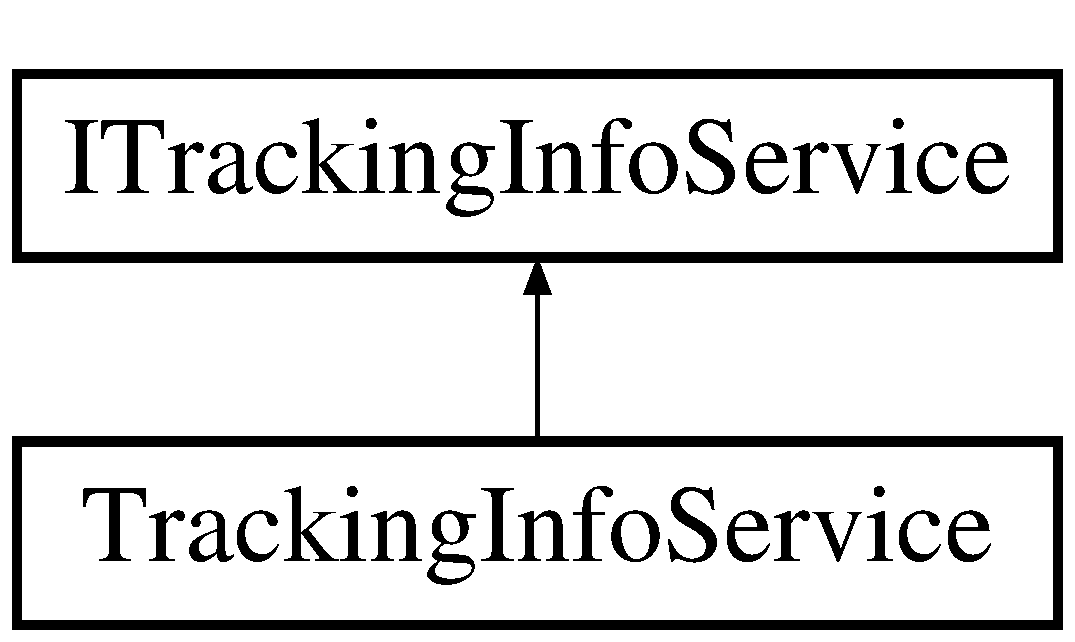
\includegraphics[height=2.000000cm]{interfaceWildLifeTracker_1_1Services_1_1ITrackingInfoService}
\end{center}
\end{figure}
\subsection*{Public Member Functions}
\begin{DoxyCompactItemize}
\item 
\hyperlink{classWildLifeTracker_1_1Models_1_1GPSTrackingInfo}{G\+P\+S\+Tracking\+Info} \hyperlink{interfaceWildLifeTracker_1_1Services_1_1ITrackingInfoService_a25bb0b990b8fd5649a97a10d14faecd2}{Add\+Tracking} (\hyperlink{classWildLifeTracker_1_1Models_1_1GPSTrackingInfo}{G\+P\+S\+Tracking\+Info} gps\+Details)
\begin{DoxyCompactList}\small\item\em Adds a new tracking info. 
\begin{DoxyParams}{Parameters}
{\em gps\+Details} & The G\+PS details to be added\\
\hline
\end{DoxyParams}
\begin{DoxyReturn}{Returns}
Returns the gps details for the newly created G\+PS info or throws Exception if there is error
\end{DoxyReturn}
\end{DoxyCompactList}\item 
\hyperlink{classWildLifeTracker_1_1Response_1_1TrackingInfoResponse}{Tracking\+Info\+Response} \hyperlink{interfaceWildLifeTracker_1_1Services_1_1ITrackingInfoService_a858073f81f74fcdf93b69fe464b13e84}{Get\+All\+Animals\+Location} ()
\begin{DoxyCompactList}\small\item\em Retrieves the latest position of the animals for all the category. \begin{DoxyReturn}{Returns}
Returns the latest G\+PS position for all animals in all category
\end{DoxyReturn}
\end{DoxyCompactList}\item 
\hyperlink{classWildLifeTracker_1_1Response_1_1TrackingInfoResponse}{Tracking\+Info\+Response} \hyperlink{interfaceWildLifeTracker_1_1Services_1_1ITrackingInfoService_af4b4cf67d3e3a8ec3e01041262c8f13a}{Get\+Animals\+Location\+Per\+Category} (string category\+Id)
\begin{DoxyCompactList}\small\item\em Retrieves the latest position of the animals when the category is specified. 
\begin{DoxyParams}{Parameters}
{\em category\+Id} & The category Id\\
\hline
\end{DoxyParams}
\begin{DoxyReturn}{Returns}
Returns the latest G\+PS position for the selected category
\end{DoxyReturn}
\end{DoxyCompactList}\end{DoxyCompactItemize}


\subsection{Detailed Description}
The interface exposes all the A\+P\+Is for tracking details 



\subsection{Member Function Documentation}
\mbox{\Hypertarget{interfaceWildLifeTracker_1_1Services_1_1ITrackingInfoService_a25bb0b990b8fd5649a97a10d14faecd2}\label{interfaceWildLifeTracker_1_1Services_1_1ITrackingInfoService_a25bb0b990b8fd5649a97a10d14faecd2}} 
\index{Wild\+Life\+Tracker\+::\+Services\+::\+I\+Tracking\+Info\+Service@{Wild\+Life\+Tracker\+::\+Services\+::\+I\+Tracking\+Info\+Service}!Add\+Tracking@{Add\+Tracking}}
\index{Add\+Tracking@{Add\+Tracking}!Wild\+Life\+Tracker\+::\+Services\+::\+I\+Tracking\+Info\+Service@{Wild\+Life\+Tracker\+::\+Services\+::\+I\+Tracking\+Info\+Service}}
\subsubsection{\texorpdfstring{Add\+Tracking()}{AddTracking()}}
{\footnotesize\ttfamily \hyperlink{classWildLifeTracker_1_1Models_1_1GPSTrackingInfo}{G\+P\+S\+Tracking\+Info} Add\+Tracking (\begin{DoxyParamCaption}\item[{\hyperlink{classWildLifeTracker_1_1Models_1_1GPSTrackingInfo}{G\+P\+S\+Tracking\+Info}}]{gps\+Details }\end{DoxyParamCaption})}



Adds a new tracking info. 
\begin{DoxyParams}{Parameters}
{\em gps\+Details} & The G\+PS details to be added\\
\hline
\end{DoxyParams}
\begin{DoxyReturn}{Returns}
Returns the gps details for the newly created G\+PS info or throws Exception if there is error
\end{DoxyReturn}




Implemented in \hyperlink{classWildLifeTracker_1_1Services_1_1TrackingInfoService_a25bb0b990b8fd5649a97a10d14faecd2}{Tracking\+Info\+Service}.

\mbox{\Hypertarget{interfaceWildLifeTracker_1_1Services_1_1ITrackingInfoService_a858073f81f74fcdf93b69fe464b13e84}\label{interfaceWildLifeTracker_1_1Services_1_1ITrackingInfoService_a858073f81f74fcdf93b69fe464b13e84}} 
\index{Wild\+Life\+Tracker\+::\+Services\+::\+I\+Tracking\+Info\+Service@{Wild\+Life\+Tracker\+::\+Services\+::\+I\+Tracking\+Info\+Service}!Get\+All\+Animals\+Location@{Get\+All\+Animals\+Location}}
\index{Get\+All\+Animals\+Location@{Get\+All\+Animals\+Location}!Wild\+Life\+Tracker\+::\+Services\+::\+I\+Tracking\+Info\+Service@{Wild\+Life\+Tracker\+::\+Services\+::\+I\+Tracking\+Info\+Service}}
\subsubsection{\texorpdfstring{Get\+All\+Animals\+Location()}{GetAllAnimalsLocation()}}
{\footnotesize\ttfamily \hyperlink{classWildLifeTracker_1_1Response_1_1TrackingInfoResponse}{Tracking\+Info\+Response} Get\+All\+Animals\+Location (\begin{DoxyParamCaption}{ }\end{DoxyParamCaption})}



Retrieves the latest position of the animals for all the category. \begin{DoxyReturn}{Returns}
Returns the latest G\+PS position for all animals in all category
\end{DoxyReturn}




Implemented in \hyperlink{classWildLifeTracker_1_1Services_1_1TrackingInfoService_a858073f81f74fcdf93b69fe464b13e84}{Tracking\+Info\+Service}.

\mbox{\Hypertarget{interfaceWildLifeTracker_1_1Services_1_1ITrackingInfoService_af4b4cf67d3e3a8ec3e01041262c8f13a}\label{interfaceWildLifeTracker_1_1Services_1_1ITrackingInfoService_af4b4cf67d3e3a8ec3e01041262c8f13a}} 
\index{Wild\+Life\+Tracker\+::\+Services\+::\+I\+Tracking\+Info\+Service@{Wild\+Life\+Tracker\+::\+Services\+::\+I\+Tracking\+Info\+Service}!Get\+Animals\+Location\+Per\+Category@{Get\+Animals\+Location\+Per\+Category}}
\index{Get\+Animals\+Location\+Per\+Category@{Get\+Animals\+Location\+Per\+Category}!Wild\+Life\+Tracker\+::\+Services\+::\+I\+Tracking\+Info\+Service@{Wild\+Life\+Tracker\+::\+Services\+::\+I\+Tracking\+Info\+Service}}
\subsubsection{\texorpdfstring{Get\+Animals\+Location\+Per\+Category()}{GetAnimalsLocationPerCategory()}}
{\footnotesize\ttfamily \hyperlink{classWildLifeTracker_1_1Response_1_1TrackingInfoResponse}{Tracking\+Info\+Response} Get\+Animals\+Location\+Per\+Category (\begin{DoxyParamCaption}\item[{string}]{category\+Id }\end{DoxyParamCaption})}



Retrieves the latest position of the animals when the category is specified. 
\begin{DoxyParams}{Parameters}
{\em category\+Id} & The category Id\\
\hline
\end{DoxyParams}
\begin{DoxyReturn}{Returns}
Returns the latest G\+PS position for the selected category
\end{DoxyReturn}




Implemented in \hyperlink{classWildLifeTracker_1_1Services_1_1TrackingInfoService_af4b4cf67d3e3a8ec3e01041262c8f13a}{Tracking\+Info\+Service}.



The documentation for this interface was generated from the following file\+:\begin{DoxyCompactItemize}
\item 
Wild\+Life\+Tracker/\+Services/\hyperlink{ITrackingInfoService_8cs}{I\+Tracking\+Info\+Service.\+cs}\end{DoxyCompactItemize}

\hypertarget{classWildLifeTracker_1_1Services_1_1TrackingInfoService}{}\section{Tracking\+Info\+Service}
\label{classWildLifeTracker_1_1Services_1_1TrackingInfoService}\index{Tracking\+Info\+Service@{Tracking\+Info\+Service}}


Tracking Service to perform different operations.  


Inheritance diagram for Tracking\+Info\+Service\+:\begin{figure}[H]
\begin{center}
\leavevmode
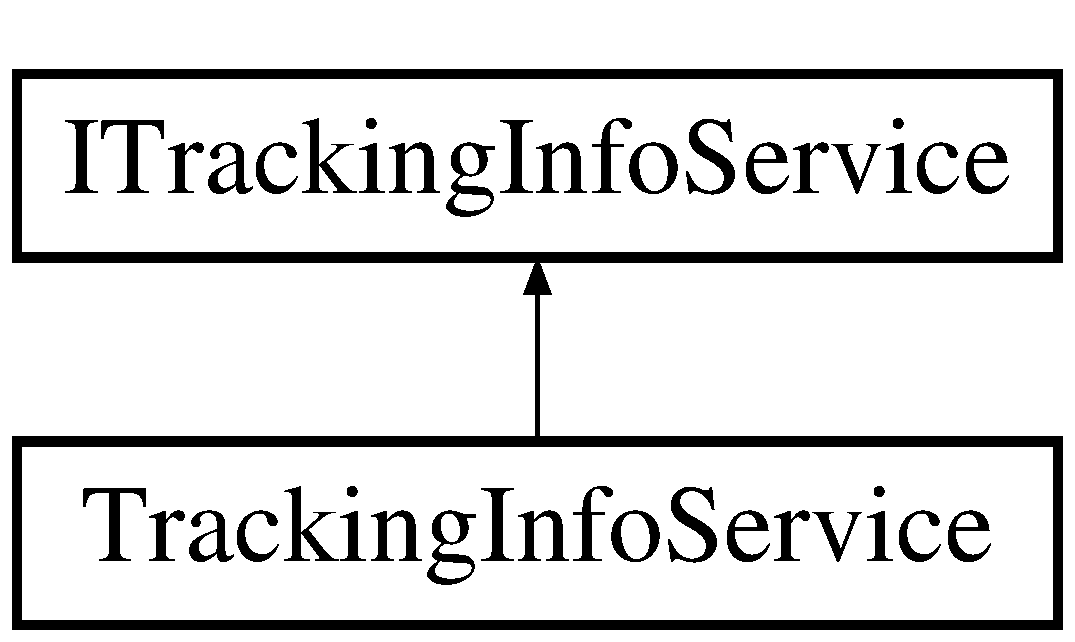
\includegraphics[height=2.000000cm]{classWildLifeTracker_1_1Services_1_1TrackingInfoService}
\end{center}
\end{figure}
\subsection*{Public Member Functions}
\begin{DoxyCompactItemize}
\item 
\hyperlink{classWildLifeTracker_1_1Services_1_1TrackingInfoService_ac3cacf8f797148311595b1403308b6cf}{Tracking\+Info\+Service} ()
\begin{DoxyCompactList}\small\item\em Constructor that intialize log4net in class \end{DoxyCompactList}\item 
\hyperlink{classWildLifeTracker_1_1Models_1_1GPSTrackingInfo}{G\+P\+S\+Tracking\+Info} \hyperlink{classWildLifeTracker_1_1Services_1_1TrackingInfoService_a25bb0b990b8fd5649a97a10d14faecd2}{Add\+Tracking} (\hyperlink{classWildLifeTracker_1_1Models_1_1GPSTrackingInfo}{G\+P\+S\+Tracking\+Info} gps\+Details)
\begin{DoxyCompactList}\small\item\em Add the tracking info (Location of animal) \end{DoxyCompactList}\item 
\hyperlink{classWildLifeTracker_1_1Response_1_1TrackingInfoResponse}{Tracking\+Info\+Response} \hyperlink{classWildLifeTracker_1_1Services_1_1TrackingInfoService_a858073f81f74fcdf93b69fe464b13e84}{Get\+All\+Animals\+Location} ()
\begin{DoxyCompactList}\small\item\em Retrieves all the animal\textquotesingle{}s latest position for all the categories \end{DoxyCompactList}\item 
\hyperlink{classWildLifeTracker_1_1Response_1_1TrackingInfoResponse}{Tracking\+Info\+Response} \hyperlink{classWildLifeTracker_1_1Services_1_1TrackingInfoService_af4b4cf67d3e3a8ec3e01041262c8f13a}{Get\+Animals\+Location\+Per\+Category} (string category\+Id)
\begin{DoxyCompactList}\small\item\em Retrieves all the animal\textquotesingle{}s latest position for the selected category \end{DoxyCompactList}\end{DoxyCompactItemize}
\subsection*{Private Attributes}
\begin{DoxyCompactItemize}
\item 
\hyperlink{classWildLifeTracker_1_1Repository_1_1TrackingRepo}{Tracking\+Repo} \hyperlink{classWildLifeTracker_1_1Services_1_1TrackingInfoService_a06c9afa34640dfb7799f60c2bf14f821}{tracking\+Repo} = null
\end{DoxyCompactItemize}


\subsection{Detailed Description}
Tracking Service to perform different operations. 



\subsection{Constructor \& Destructor Documentation}
\mbox{\Hypertarget{classWildLifeTracker_1_1Services_1_1TrackingInfoService_ac3cacf8f797148311595b1403308b6cf}\label{classWildLifeTracker_1_1Services_1_1TrackingInfoService_ac3cacf8f797148311595b1403308b6cf}} 
\index{Wild\+Life\+Tracker\+::\+Services\+::\+Tracking\+Info\+Service@{Wild\+Life\+Tracker\+::\+Services\+::\+Tracking\+Info\+Service}!Tracking\+Info\+Service@{Tracking\+Info\+Service}}
\index{Tracking\+Info\+Service@{Tracking\+Info\+Service}!Wild\+Life\+Tracker\+::\+Services\+::\+Tracking\+Info\+Service@{Wild\+Life\+Tracker\+::\+Services\+::\+Tracking\+Info\+Service}}
\subsubsection{\texorpdfstring{Tracking\+Info\+Service()}{TrackingInfoService()}}
{\footnotesize\ttfamily \hyperlink{classWildLifeTracker_1_1Services_1_1TrackingInfoService}{Tracking\+Info\+Service} (\begin{DoxyParamCaption}{ }\end{DoxyParamCaption})\hspace{0.3cm}{\ttfamily [inline]}}



Constructor that intialize log4net in class 



\subsection{Member Function Documentation}
\mbox{\Hypertarget{classWildLifeTracker_1_1Services_1_1TrackingInfoService_a25bb0b990b8fd5649a97a10d14faecd2}\label{classWildLifeTracker_1_1Services_1_1TrackingInfoService_a25bb0b990b8fd5649a97a10d14faecd2}} 
\index{Wild\+Life\+Tracker\+::\+Services\+::\+Tracking\+Info\+Service@{Wild\+Life\+Tracker\+::\+Services\+::\+Tracking\+Info\+Service}!Add\+Tracking@{Add\+Tracking}}
\index{Add\+Tracking@{Add\+Tracking}!Wild\+Life\+Tracker\+::\+Services\+::\+Tracking\+Info\+Service@{Wild\+Life\+Tracker\+::\+Services\+::\+Tracking\+Info\+Service}}
\subsubsection{\texorpdfstring{Add\+Tracking()}{AddTracking()}}
{\footnotesize\ttfamily \hyperlink{classWildLifeTracker_1_1Models_1_1GPSTrackingInfo}{G\+P\+S\+Tracking\+Info} Add\+Tracking (\begin{DoxyParamCaption}\item[{\hyperlink{classWildLifeTracker_1_1Models_1_1GPSTrackingInfo}{G\+P\+S\+Tracking\+Info}}]{gps\+Details }\end{DoxyParamCaption})\hspace{0.3cm}{\ttfamily [inline]}}



Add the tracking info (Location of animal) 


\begin{DoxyParams}{Parameters}
{\em animal\+Details} & The animal details\\
\hline
\end{DoxyParams}
\begin{DoxyReturn}{Returns}
The details of animal that is added
\end{DoxyReturn}


Implements \hyperlink{interfaceWildLifeTracker_1_1Services_1_1ITrackingInfoService_a25bb0b990b8fd5649a97a10d14faecd2}{I\+Tracking\+Info\+Service}.

\mbox{\Hypertarget{classWildLifeTracker_1_1Services_1_1TrackingInfoService_a858073f81f74fcdf93b69fe464b13e84}\label{classWildLifeTracker_1_1Services_1_1TrackingInfoService_a858073f81f74fcdf93b69fe464b13e84}} 
\index{Wild\+Life\+Tracker\+::\+Services\+::\+Tracking\+Info\+Service@{Wild\+Life\+Tracker\+::\+Services\+::\+Tracking\+Info\+Service}!Get\+All\+Animals\+Location@{Get\+All\+Animals\+Location}}
\index{Get\+All\+Animals\+Location@{Get\+All\+Animals\+Location}!Wild\+Life\+Tracker\+::\+Services\+::\+Tracking\+Info\+Service@{Wild\+Life\+Tracker\+::\+Services\+::\+Tracking\+Info\+Service}}
\subsubsection{\texorpdfstring{Get\+All\+Animals\+Location()}{GetAllAnimalsLocation()}}
{\footnotesize\ttfamily \hyperlink{classWildLifeTracker_1_1Response_1_1TrackingInfoResponse}{Tracking\+Info\+Response} Get\+All\+Animals\+Location (\begin{DoxyParamCaption}{ }\end{DoxyParamCaption})\hspace{0.3cm}{\ttfamily [inline]}}



Retrieves all the animal\textquotesingle{}s latest position for all the categories 

\begin{DoxyReturn}{Returns}
Details of animals, category and the tracking information of all the animals in all category
\end{DoxyReturn}


Implements \hyperlink{interfaceWildLifeTracker_1_1Services_1_1ITrackingInfoService_a858073f81f74fcdf93b69fe464b13e84}{I\+Tracking\+Info\+Service}.

\mbox{\Hypertarget{classWildLifeTracker_1_1Services_1_1TrackingInfoService_af4b4cf67d3e3a8ec3e01041262c8f13a}\label{classWildLifeTracker_1_1Services_1_1TrackingInfoService_af4b4cf67d3e3a8ec3e01041262c8f13a}} 
\index{Wild\+Life\+Tracker\+::\+Services\+::\+Tracking\+Info\+Service@{Wild\+Life\+Tracker\+::\+Services\+::\+Tracking\+Info\+Service}!Get\+Animals\+Location\+Per\+Category@{Get\+Animals\+Location\+Per\+Category}}
\index{Get\+Animals\+Location\+Per\+Category@{Get\+Animals\+Location\+Per\+Category}!Wild\+Life\+Tracker\+::\+Services\+::\+Tracking\+Info\+Service@{Wild\+Life\+Tracker\+::\+Services\+::\+Tracking\+Info\+Service}}
\subsubsection{\texorpdfstring{Get\+Animals\+Location\+Per\+Category()}{GetAnimalsLocationPerCategory()}}
{\footnotesize\ttfamily \hyperlink{classWildLifeTracker_1_1Response_1_1TrackingInfoResponse}{Tracking\+Info\+Response} Get\+Animals\+Location\+Per\+Category (\begin{DoxyParamCaption}\item[{string}]{category\+Id }\end{DoxyParamCaption})\hspace{0.3cm}{\ttfamily [inline]}}



Retrieves all the animal\textquotesingle{}s latest position for the selected category 

\begin{DoxyReturn}{Returns}
Details of animals, category and the tracking information of all the animals in selected category
\end{DoxyReturn}


Implements \hyperlink{interfaceWildLifeTracker_1_1Services_1_1ITrackingInfoService_af4b4cf67d3e3a8ec3e01041262c8f13a}{I\+Tracking\+Info\+Service}.



\subsection{Member Data Documentation}
\mbox{\Hypertarget{classWildLifeTracker_1_1Services_1_1TrackingInfoService_a06c9afa34640dfb7799f60c2bf14f821}\label{classWildLifeTracker_1_1Services_1_1TrackingInfoService_a06c9afa34640dfb7799f60c2bf14f821}} 
\index{Wild\+Life\+Tracker\+::\+Services\+::\+Tracking\+Info\+Service@{Wild\+Life\+Tracker\+::\+Services\+::\+Tracking\+Info\+Service}!tracking\+Repo@{tracking\+Repo}}
\index{tracking\+Repo@{tracking\+Repo}!Wild\+Life\+Tracker\+::\+Services\+::\+Tracking\+Info\+Service@{Wild\+Life\+Tracker\+::\+Services\+::\+Tracking\+Info\+Service}}
\subsubsection{\texorpdfstring{tracking\+Repo}{trackingRepo}}
{\footnotesize\ttfamily \hyperlink{classWildLifeTracker_1_1Repository_1_1TrackingRepo}{Tracking\+Repo} tracking\+Repo = null\hspace{0.3cm}{\ttfamily [private]}}



The documentation for this class was generated from the following file\+:\begin{DoxyCompactItemize}
\item 
Wild\+Life\+Tracker/\+Services/\hyperlink{TrackingInfoService_8svc_8cs}{Tracking\+Info\+Service.\+svc.\+cs}\end{DoxyCompactItemize}

\hypertarget{classWildLifeTracker_1_1tblanimal}{}\section{tblanimal}
\label{classWildLifeTracker_1_1tblanimal}\index{tblanimal@{tblanimal}}
\subsection*{Public Member Functions}
\begin{DoxyCompactItemize}
\item 
\hyperlink{classWildLifeTracker_1_1tblanimal_a076509de34d3d07100194a5dd3f191c9}{tblanimal} ()
\end{DoxyCompactItemize}
\subsection*{Properties}
\begin{DoxyCompactItemize}
\item 
int \hyperlink{classWildLifeTracker_1_1tblanimal_a99787b9867ae390df467a99040589a55}{animal\+Id}\hspace{0.3cm}{\ttfamily  \mbox{[}get, set\mbox{]}}
\item 
string \hyperlink{classWildLifeTracker_1_1tblanimal_afd38ba6641283469fc9e94212467f9a2}{animal\+Name}\hspace{0.3cm}{\ttfamily  \mbox{[}get, set\mbox{]}}
\item 
int \hyperlink{classWildLifeTracker_1_1tblanimal_a423f91c56dc35040d661cfbe357f7c78}{category\+Id}\hspace{0.3cm}{\ttfamily  \mbox{[}get, set\mbox{]}}
\item 
System.\+Date\+Time \hyperlink{classWildLifeTracker_1_1tblanimal_a0da6329d5fbb1b91739557ad49ece9c0}{created\+At}\hspace{0.3cm}{\ttfamily  \mbox{[}get, set\mbox{]}}
\item 
string \hyperlink{classWildLifeTracker_1_1tblanimal_a073b88a9702ca0513fa534f58a048070}{gps\+Device\+Id}\hspace{0.3cm}{\ttfamily  \mbox{[}get, set\mbox{]}}
\item 
virtual \hyperlink{classWildLifeTracker_1_1tblcategory}{tblcategory} \hyperlink{classWildLifeTracker_1_1tblanimal_aea411632582d5ca6da0cfd6f0b3eadfd}{tblcategory}\hspace{0.3cm}{\ttfamily  \mbox{[}get, set\mbox{]}}
\item 
virtual I\+Collection$<$ \hyperlink{classWildLifeTracker_1_1tblgpstracking}{tblgpstracking} $>$ \hyperlink{classWildLifeTracker_1_1tblanimal_af00c7cc8fc89df2b998c54b894a5d5c5}{tblgpstrackings}\hspace{0.3cm}{\ttfamily  \mbox{[}get, set\mbox{]}}
\end{DoxyCompactItemize}


\subsection{Constructor \& Destructor Documentation}
\mbox{\Hypertarget{classWildLifeTracker_1_1tblanimal_a076509de34d3d07100194a5dd3f191c9}\label{classWildLifeTracker_1_1tblanimal_a076509de34d3d07100194a5dd3f191c9}} 
\index{Wild\+Life\+Tracker\+::tblanimal@{Wild\+Life\+Tracker\+::tblanimal}!tblanimal@{tblanimal}}
\index{tblanimal@{tblanimal}!Wild\+Life\+Tracker\+::tblanimal@{Wild\+Life\+Tracker\+::tblanimal}}
\subsubsection{\texorpdfstring{tblanimal()}{tblanimal()}}
{\footnotesize\ttfamily \hyperlink{classWildLifeTracker_1_1tblanimal}{tblanimal} (\begin{DoxyParamCaption}{ }\end{DoxyParamCaption})\hspace{0.3cm}{\ttfamily [inline]}}



\subsection{Property Documentation}
\mbox{\Hypertarget{classWildLifeTracker_1_1tblanimal_a99787b9867ae390df467a99040589a55}\label{classWildLifeTracker_1_1tblanimal_a99787b9867ae390df467a99040589a55}} 
\index{Wild\+Life\+Tracker\+::tblanimal@{Wild\+Life\+Tracker\+::tblanimal}!animal\+Id@{animal\+Id}}
\index{animal\+Id@{animal\+Id}!Wild\+Life\+Tracker\+::tblanimal@{Wild\+Life\+Tracker\+::tblanimal}}
\subsubsection{\texorpdfstring{animal\+Id}{animalId}}
{\footnotesize\ttfamily int animal\+Id\hspace{0.3cm}{\ttfamily [get]}, {\ttfamily [set]}}

\mbox{\Hypertarget{classWildLifeTracker_1_1tblanimal_afd38ba6641283469fc9e94212467f9a2}\label{classWildLifeTracker_1_1tblanimal_afd38ba6641283469fc9e94212467f9a2}} 
\index{Wild\+Life\+Tracker\+::tblanimal@{Wild\+Life\+Tracker\+::tblanimal}!animal\+Name@{animal\+Name}}
\index{animal\+Name@{animal\+Name}!Wild\+Life\+Tracker\+::tblanimal@{Wild\+Life\+Tracker\+::tblanimal}}
\subsubsection{\texorpdfstring{animal\+Name}{animalName}}
{\footnotesize\ttfamily string animal\+Name\hspace{0.3cm}{\ttfamily [get]}, {\ttfamily [set]}}

\mbox{\Hypertarget{classWildLifeTracker_1_1tblanimal_a423f91c56dc35040d661cfbe357f7c78}\label{classWildLifeTracker_1_1tblanimal_a423f91c56dc35040d661cfbe357f7c78}} 
\index{Wild\+Life\+Tracker\+::tblanimal@{Wild\+Life\+Tracker\+::tblanimal}!category\+Id@{category\+Id}}
\index{category\+Id@{category\+Id}!Wild\+Life\+Tracker\+::tblanimal@{Wild\+Life\+Tracker\+::tblanimal}}
\subsubsection{\texorpdfstring{category\+Id}{categoryId}}
{\footnotesize\ttfamily int category\+Id\hspace{0.3cm}{\ttfamily [get]}, {\ttfamily [set]}}

\mbox{\Hypertarget{classWildLifeTracker_1_1tblanimal_a0da6329d5fbb1b91739557ad49ece9c0}\label{classWildLifeTracker_1_1tblanimal_a0da6329d5fbb1b91739557ad49ece9c0}} 
\index{Wild\+Life\+Tracker\+::tblanimal@{Wild\+Life\+Tracker\+::tblanimal}!created\+At@{created\+At}}
\index{created\+At@{created\+At}!Wild\+Life\+Tracker\+::tblanimal@{Wild\+Life\+Tracker\+::tblanimal}}
\subsubsection{\texorpdfstring{created\+At}{createdAt}}
{\footnotesize\ttfamily System.\+Date\+Time created\+At\hspace{0.3cm}{\ttfamily [get]}, {\ttfamily [set]}}

\mbox{\Hypertarget{classWildLifeTracker_1_1tblanimal_a073b88a9702ca0513fa534f58a048070}\label{classWildLifeTracker_1_1tblanimal_a073b88a9702ca0513fa534f58a048070}} 
\index{Wild\+Life\+Tracker\+::tblanimal@{Wild\+Life\+Tracker\+::tblanimal}!gps\+Device\+Id@{gps\+Device\+Id}}
\index{gps\+Device\+Id@{gps\+Device\+Id}!Wild\+Life\+Tracker\+::tblanimal@{Wild\+Life\+Tracker\+::tblanimal}}
\subsubsection{\texorpdfstring{gps\+Device\+Id}{gpsDeviceId}}
{\footnotesize\ttfamily string gps\+Device\+Id\hspace{0.3cm}{\ttfamily [get]}, {\ttfamily [set]}}

\mbox{\Hypertarget{classWildLifeTracker_1_1tblanimal_aea411632582d5ca6da0cfd6f0b3eadfd}\label{classWildLifeTracker_1_1tblanimal_aea411632582d5ca6da0cfd6f0b3eadfd}} 
\index{Wild\+Life\+Tracker\+::tblanimal@{Wild\+Life\+Tracker\+::tblanimal}!tblcategory@{tblcategory}}
\index{tblcategory@{tblcategory}!Wild\+Life\+Tracker\+::tblanimal@{Wild\+Life\+Tracker\+::tblanimal}}
\subsubsection{\texorpdfstring{tblcategory}{tblcategory}}
{\footnotesize\ttfamily virtual \hyperlink{classWildLifeTracker_1_1tblcategory}{tblcategory} \hyperlink{classWildLifeTracker_1_1tblcategory}{tblcategory}\hspace{0.3cm}{\ttfamily [get]}, {\ttfamily [set]}}

\mbox{\Hypertarget{classWildLifeTracker_1_1tblanimal_af00c7cc8fc89df2b998c54b894a5d5c5}\label{classWildLifeTracker_1_1tblanimal_af00c7cc8fc89df2b998c54b894a5d5c5}} 
\index{Wild\+Life\+Tracker\+::tblanimal@{Wild\+Life\+Tracker\+::tblanimal}!tblgpstrackings@{tblgpstrackings}}
\index{tblgpstrackings@{tblgpstrackings}!Wild\+Life\+Tracker\+::tblanimal@{Wild\+Life\+Tracker\+::tblanimal}}
\subsubsection{\texorpdfstring{tblgpstrackings}{tblgpstrackings}}
{\footnotesize\ttfamily virtual I\+Collection$<$\hyperlink{classWildLifeTracker_1_1tblgpstracking}{tblgpstracking}$>$ tblgpstrackings\hspace{0.3cm}{\ttfamily [get]}, {\ttfamily [set]}}



The documentation for this class was generated from the following file\+:\begin{DoxyCompactItemize}
\item 
Wild\+Life\+Tracker/\hyperlink{tblanimal_8cs}{tblanimal.\+cs}\end{DoxyCompactItemize}

\hypertarget{classWildLifeTracker_1_1tblcategory}{}\section{tblcategory}
\label{classWildLifeTracker_1_1tblcategory}\index{tblcategory@{tblcategory}}
\subsection*{Public Member Functions}
\begin{DoxyCompactItemize}
\item 
\hyperlink{classWildLifeTracker_1_1tblcategory_a1a4ae07dab4a80f5272e38cd3d0b2e19}{tblcategory} ()
\end{DoxyCompactItemize}
\subsection*{Properties}
\begin{DoxyCompactItemize}
\item 
string \hyperlink{classWildLifeTracker_1_1tblcategory_ae992743f1fc0d9386b609d8871a4bd6b}{category\+Desc}\hspace{0.3cm}{\ttfamily  \mbox{[}get, set\mbox{]}}
\item 
int \hyperlink{classWildLifeTracker_1_1tblcategory_a423f91c56dc35040d661cfbe357f7c78}{category\+Id}\hspace{0.3cm}{\ttfamily  \mbox{[}get, set\mbox{]}}
\item 
string \hyperlink{classWildLifeTracker_1_1tblcategory_a1eca787c85e1bc45b49bbd281d4106fd}{category\+Name}\hspace{0.3cm}{\ttfamily  \mbox{[}get, set\mbox{]}}
\item 
string \hyperlink{classWildLifeTracker_1_1tblcategory_a0ecdefcc99a4b41b1ef3a04167756366}{color\+Indication}\hspace{0.3cm}{\ttfamily  \mbox{[}get, set\mbox{]}}
\item 
virtual I\+Collection$<$ \hyperlink{classWildLifeTracker_1_1tblanimal}{tblanimal} $>$ \hyperlink{classWildLifeTracker_1_1tblcategory_acde66266ee81c53bf73df2c0b3be64c2}{tblanimals}\hspace{0.3cm}{\ttfamily  \mbox{[}get, set\mbox{]}}
\end{DoxyCompactItemize}


\subsection{Constructor \& Destructor Documentation}
\mbox{\Hypertarget{classWildLifeTracker_1_1tblcategory_a1a4ae07dab4a80f5272e38cd3d0b2e19}\label{classWildLifeTracker_1_1tblcategory_a1a4ae07dab4a80f5272e38cd3d0b2e19}} 
\index{Wild\+Life\+Tracker\+::tblcategory@{Wild\+Life\+Tracker\+::tblcategory}!tblcategory@{tblcategory}}
\index{tblcategory@{tblcategory}!Wild\+Life\+Tracker\+::tblcategory@{Wild\+Life\+Tracker\+::tblcategory}}
\subsubsection{\texorpdfstring{tblcategory()}{tblcategory()}}
{\footnotesize\ttfamily \hyperlink{classWildLifeTracker_1_1tblcategory}{tblcategory} (\begin{DoxyParamCaption}{ }\end{DoxyParamCaption})\hspace{0.3cm}{\ttfamily [inline]}}



\subsection{Property Documentation}
\mbox{\Hypertarget{classWildLifeTracker_1_1tblcategory_ae992743f1fc0d9386b609d8871a4bd6b}\label{classWildLifeTracker_1_1tblcategory_ae992743f1fc0d9386b609d8871a4bd6b}} 
\index{Wild\+Life\+Tracker\+::tblcategory@{Wild\+Life\+Tracker\+::tblcategory}!category\+Desc@{category\+Desc}}
\index{category\+Desc@{category\+Desc}!Wild\+Life\+Tracker\+::tblcategory@{Wild\+Life\+Tracker\+::tblcategory}}
\subsubsection{\texorpdfstring{category\+Desc}{categoryDesc}}
{\footnotesize\ttfamily string category\+Desc\hspace{0.3cm}{\ttfamily [get]}, {\ttfamily [set]}}

\mbox{\Hypertarget{classWildLifeTracker_1_1tblcategory_a423f91c56dc35040d661cfbe357f7c78}\label{classWildLifeTracker_1_1tblcategory_a423f91c56dc35040d661cfbe357f7c78}} 
\index{Wild\+Life\+Tracker\+::tblcategory@{Wild\+Life\+Tracker\+::tblcategory}!category\+Id@{category\+Id}}
\index{category\+Id@{category\+Id}!Wild\+Life\+Tracker\+::tblcategory@{Wild\+Life\+Tracker\+::tblcategory}}
\subsubsection{\texorpdfstring{category\+Id}{categoryId}}
{\footnotesize\ttfamily int category\+Id\hspace{0.3cm}{\ttfamily [get]}, {\ttfamily [set]}}

\mbox{\Hypertarget{classWildLifeTracker_1_1tblcategory_a1eca787c85e1bc45b49bbd281d4106fd}\label{classWildLifeTracker_1_1tblcategory_a1eca787c85e1bc45b49bbd281d4106fd}} 
\index{Wild\+Life\+Tracker\+::tblcategory@{Wild\+Life\+Tracker\+::tblcategory}!category\+Name@{category\+Name}}
\index{category\+Name@{category\+Name}!Wild\+Life\+Tracker\+::tblcategory@{Wild\+Life\+Tracker\+::tblcategory}}
\subsubsection{\texorpdfstring{category\+Name}{categoryName}}
{\footnotesize\ttfamily string category\+Name\hspace{0.3cm}{\ttfamily [get]}, {\ttfamily [set]}}

\mbox{\Hypertarget{classWildLifeTracker_1_1tblcategory_a0ecdefcc99a4b41b1ef3a04167756366}\label{classWildLifeTracker_1_1tblcategory_a0ecdefcc99a4b41b1ef3a04167756366}} 
\index{Wild\+Life\+Tracker\+::tblcategory@{Wild\+Life\+Tracker\+::tblcategory}!color\+Indication@{color\+Indication}}
\index{color\+Indication@{color\+Indication}!Wild\+Life\+Tracker\+::tblcategory@{Wild\+Life\+Tracker\+::tblcategory}}
\subsubsection{\texorpdfstring{color\+Indication}{colorIndication}}
{\footnotesize\ttfamily string color\+Indication\hspace{0.3cm}{\ttfamily [get]}, {\ttfamily [set]}}

\mbox{\Hypertarget{classWildLifeTracker_1_1tblcategory_acde66266ee81c53bf73df2c0b3be64c2}\label{classWildLifeTracker_1_1tblcategory_acde66266ee81c53bf73df2c0b3be64c2}} 
\index{Wild\+Life\+Tracker\+::tblcategory@{Wild\+Life\+Tracker\+::tblcategory}!tblanimals@{tblanimals}}
\index{tblanimals@{tblanimals}!Wild\+Life\+Tracker\+::tblcategory@{Wild\+Life\+Tracker\+::tblcategory}}
\subsubsection{\texorpdfstring{tblanimals}{tblanimals}}
{\footnotesize\ttfamily virtual I\+Collection$<$\hyperlink{classWildLifeTracker_1_1tblanimal}{tblanimal}$>$ tblanimals\hspace{0.3cm}{\ttfamily [get]}, {\ttfamily [set]}}



The documentation for this class was generated from the following file\+:\begin{DoxyCompactItemize}
\item 
Wild\+Life\+Tracker/\hyperlink{tblcategory_8cs}{tblcategory.\+cs}\end{DoxyCompactItemize}

\hypertarget{classWildLifeTracker_1_1tblgpstracking}{}\section{tblgpstracking}
\label{classWildLifeTracker_1_1tblgpstracking}\index{tblgpstracking@{tblgpstracking}}
\subsection*{Properties}
\begin{DoxyCompactItemize}
\item 
int \hyperlink{classWildLifeTracker_1_1tblgpstracking_a99787b9867ae390df467a99040589a55}{animal\+Id}\hspace{0.3cm}{\ttfamily  \mbox{[}get, set\mbox{]}}
\item 
System.\+Date\+Time \hyperlink{classWildLifeTracker_1_1tblgpstracking_a0da6329d5fbb1b91739557ad49ece9c0}{created\+At}\hspace{0.3cm}{\ttfamily  \mbox{[}get, set\mbox{]}}
\item 
double \hyperlink{classWildLifeTracker_1_1tblgpstracking_a76714bdbc5c536fa77dfb14533ff82a9}{latitude}\hspace{0.3cm}{\ttfamily  \mbox{[}get, set\mbox{]}}
\item 
double \hyperlink{classWildLifeTracker_1_1tblgpstracking_ac155e35fdeebafc89723a51520fb9fe6}{longitude}\hspace{0.3cm}{\ttfamily  \mbox{[}get, set\mbox{]}}
\item 
virtual \hyperlink{classWildLifeTracker_1_1tblanimal}{tblanimal} \hyperlink{classWildLifeTracker_1_1tblgpstracking_ac15c6239223b3b3eea8fa42336daa5bd}{tblanimal}\hspace{0.3cm}{\ttfamily  \mbox{[}get, set\mbox{]}}
\item 
int \hyperlink{classWildLifeTracker_1_1tblgpstracking_a7291076f1fbf1ead00eb6c30cf33d943}{tracking\+Id}\hspace{0.3cm}{\ttfamily  \mbox{[}get, set\mbox{]}}
\end{DoxyCompactItemize}


\subsection{Property Documentation}
\mbox{\Hypertarget{classWildLifeTracker_1_1tblgpstracking_a99787b9867ae390df467a99040589a55}\label{classWildLifeTracker_1_1tblgpstracking_a99787b9867ae390df467a99040589a55}} 
\index{Wild\+Life\+Tracker\+::tblgpstracking@{Wild\+Life\+Tracker\+::tblgpstracking}!animal\+Id@{animal\+Id}}
\index{animal\+Id@{animal\+Id}!Wild\+Life\+Tracker\+::tblgpstracking@{Wild\+Life\+Tracker\+::tblgpstracking}}
\subsubsection{\texorpdfstring{animal\+Id}{animalId}}
{\footnotesize\ttfamily int animal\+Id\hspace{0.3cm}{\ttfamily [get]}, {\ttfamily [set]}}

\mbox{\Hypertarget{classWildLifeTracker_1_1tblgpstracking_a0da6329d5fbb1b91739557ad49ece9c0}\label{classWildLifeTracker_1_1tblgpstracking_a0da6329d5fbb1b91739557ad49ece9c0}} 
\index{Wild\+Life\+Tracker\+::tblgpstracking@{Wild\+Life\+Tracker\+::tblgpstracking}!created\+At@{created\+At}}
\index{created\+At@{created\+At}!Wild\+Life\+Tracker\+::tblgpstracking@{Wild\+Life\+Tracker\+::tblgpstracking}}
\subsubsection{\texorpdfstring{created\+At}{createdAt}}
{\footnotesize\ttfamily System.\+Date\+Time created\+At\hspace{0.3cm}{\ttfamily [get]}, {\ttfamily [set]}}

\mbox{\Hypertarget{classWildLifeTracker_1_1tblgpstracking_a76714bdbc5c536fa77dfb14533ff82a9}\label{classWildLifeTracker_1_1tblgpstracking_a76714bdbc5c536fa77dfb14533ff82a9}} 
\index{Wild\+Life\+Tracker\+::tblgpstracking@{Wild\+Life\+Tracker\+::tblgpstracking}!latitude@{latitude}}
\index{latitude@{latitude}!Wild\+Life\+Tracker\+::tblgpstracking@{Wild\+Life\+Tracker\+::tblgpstracking}}
\subsubsection{\texorpdfstring{latitude}{latitude}}
{\footnotesize\ttfamily double latitude\hspace{0.3cm}{\ttfamily [get]}, {\ttfamily [set]}}

\mbox{\Hypertarget{classWildLifeTracker_1_1tblgpstracking_ac155e35fdeebafc89723a51520fb9fe6}\label{classWildLifeTracker_1_1tblgpstracking_ac155e35fdeebafc89723a51520fb9fe6}} 
\index{Wild\+Life\+Tracker\+::tblgpstracking@{Wild\+Life\+Tracker\+::tblgpstracking}!longitude@{longitude}}
\index{longitude@{longitude}!Wild\+Life\+Tracker\+::tblgpstracking@{Wild\+Life\+Tracker\+::tblgpstracking}}
\subsubsection{\texorpdfstring{longitude}{longitude}}
{\footnotesize\ttfamily double longitude\hspace{0.3cm}{\ttfamily [get]}, {\ttfamily [set]}}

\mbox{\Hypertarget{classWildLifeTracker_1_1tblgpstracking_ac15c6239223b3b3eea8fa42336daa5bd}\label{classWildLifeTracker_1_1tblgpstracking_ac15c6239223b3b3eea8fa42336daa5bd}} 
\index{Wild\+Life\+Tracker\+::tblgpstracking@{Wild\+Life\+Tracker\+::tblgpstracking}!tblanimal@{tblanimal}}
\index{tblanimal@{tblanimal}!Wild\+Life\+Tracker\+::tblgpstracking@{Wild\+Life\+Tracker\+::tblgpstracking}}
\subsubsection{\texorpdfstring{tblanimal}{tblanimal}}
{\footnotesize\ttfamily virtual \hyperlink{classWildLifeTracker_1_1tblanimal}{tblanimal} \hyperlink{classWildLifeTracker_1_1tblanimal}{tblanimal}\hspace{0.3cm}{\ttfamily [get]}, {\ttfamily [set]}}

\mbox{\Hypertarget{classWildLifeTracker_1_1tblgpstracking_a7291076f1fbf1ead00eb6c30cf33d943}\label{classWildLifeTracker_1_1tblgpstracking_a7291076f1fbf1ead00eb6c30cf33d943}} 
\index{Wild\+Life\+Tracker\+::tblgpstracking@{Wild\+Life\+Tracker\+::tblgpstracking}!tracking\+Id@{tracking\+Id}}
\index{tracking\+Id@{tracking\+Id}!Wild\+Life\+Tracker\+::tblgpstracking@{Wild\+Life\+Tracker\+::tblgpstracking}}
\subsubsection{\texorpdfstring{tracking\+Id}{trackingId}}
{\footnotesize\ttfamily int tracking\+Id\hspace{0.3cm}{\ttfamily [get]}, {\ttfamily [set]}}



The documentation for this class was generated from the following file\+:\begin{DoxyCompactItemize}
\item 
Wild\+Life\+Tracker/\hyperlink{tblgpstracking_8cs}{tblgpstracking.\+cs}\end{DoxyCompactItemize}

\hypertarget{classWildLifeTracker_1_1Utility_1_1ErrorHandler}{}\section{Error\+Handler}
\label{classWildLifeTracker_1_1Utility_1_1ErrorHandler}\index{Error\+Handler@{Error\+Handler}}
\subsection*{Public Member Functions}
\begin{DoxyCompactItemize}
\item 
\hyperlink{classWildLifeTracker_1_1Utility_1_1ErrorHandler_abd5196a598ed1d50314664f0993242f8}{Error\+Handler} (string error\+Message, string error\+Description)
\end{DoxyCompactItemize}
\subsection*{Properties}
\begin{DoxyCompactItemize}
\item 
string \hyperlink{classWildLifeTracker_1_1Utility_1_1ErrorHandler_a99e6e8d0590f2455a2d5df4bcd620700}{Error\+Desc}\hspace{0.3cm}{\ttfamily  \mbox{[}get, private set\mbox{]}}
\item 
string \hyperlink{classWildLifeTracker_1_1Utility_1_1ErrorHandler_abe9394119736c4856e64d035a36f987e}{error\+Mess}\hspace{0.3cm}{\ttfamily  \mbox{[}get, private set\mbox{]}}
\end{DoxyCompactItemize}


\subsection{Constructor \& Destructor Documentation}
\mbox{\Hypertarget{classWildLifeTracker_1_1Utility_1_1ErrorHandler_abd5196a598ed1d50314664f0993242f8}\label{classWildLifeTracker_1_1Utility_1_1ErrorHandler_abd5196a598ed1d50314664f0993242f8}} 
\index{Wild\+Life\+Tracker\+::\+Utility\+::\+Error\+Handler@{Wild\+Life\+Tracker\+::\+Utility\+::\+Error\+Handler}!Error\+Handler@{Error\+Handler}}
\index{Error\+Handler@{Error\+Handler}!Wild\+Life\+Tracker\+::\+Utility\+::\+Error\+Handler@{Wild\+Life\+Tracker\+::\+Utility\+::\+Error\+Handler}}
\subsubsection{\texorpdfstring{Error\+Handler()}{ErrorHandler()}}
{\footnotesize\ttfamily \hyperlink{classWildLifeTracker_1_1Utility_1_1ErrorHandler}{Error\+Handler} (\begin{DoxyParamCaption}\item[{string}]{error\+Message,  }\item[{string}]{error\+Description }\end{DoxyParamCaption})\hspace{0.3cm}{\ttfamily [inline]}}



\subsection{Property Documentation}
\mbox{\Hypertarget{classWildLifeTracker_1_1Utility_1_1ErrorHandler_a99e6e8d0590f2455a2d5df4bcd620700}\label{classWildLifeTracker_1_1Utility_1_1ErrorHandler_a99e6e8d0590f2455a2d5df4bcd620700}} 
\index{Wild\+Life\+Tracker\+::\+Utility\+::\+Error\+Handler@{Wild\+Life\+Tracker\+::\+Utility\+::\+Error\+Handler}!Error\+Desc@{Error\+Desc}}
\index{Error\+Desc@{Error\+Desc}!Wild\+Life\+Tracker\+::\+Utility\+::\+Error\+Handler@{Wild\+Life\+Tracker\+::\+Utility\+::\+Error\+Handler}}
\subsubsection{\texorpdfstring{Error\+Desc}{ErrorDesc}}
{\footnotesize\ttfamily string Error\+Desc\hspace{0.3cm}{\ttfamily [get]}, {\ttfamily [private set]}}

\mbox{\Hypertarget{classWildLifeTracker_1_1Utility_1_1ErrorHandler_abe9394119736c4856e64d035a36f987e}\label{classWildLifeTracker_1_1Utility_1_1ErrorHandler_abe9394119736c4856e64d035a36f987e}} 
\index{Wild\+Life\+Tracker\+::\+Utility\+::\+Error\+Handler@{Wild\+Life\+Tracker\+::\+Utility\+::\+Error\+Handler}!error\+Mess@{error\+Mess}}
\index{error\+Mess@{error\+Mess}!Wild\+Life\+Tracker\+::\+Utility\+::\+Error\+Handler@{Wild\+Life\+Tracker\+::\+Utility\+::\+Error\+Handler}}
\subsubsection{\texorpdfstring{error\+Mess}{errorMess}}
{\footnotesize\ttfamily string error\+Mess\hspace{0.3cm}{\ttfamily [get]}, {\ttfamily [private set]}}



The documentation for this class was generated from the following file\+:\begin{DoxyCompactItemize}
\item 
Wild\+Life\+Tracker/\+Utility/\hyperlink{ExceptionHandler_8cs}{Exception\+Handler.\+cs}\end{DoxyCompactItemize}

\chapter{File Documentation}
\hypertarget{DbModels_8Context_8cs}{}\section{Wild\+Life\+Tracker/\+Db\+Models.Context.\+cs File Reference}
\label{DbModels_8Context_8cs}\index{Wild\+Life\+Tracker/\+Db\+Models.\+Context.\+cs@{Wild\+Life\+Tracker/\+Db\+Models.\+Context.\+cs}}
\subsection*{Classes}
\begin{DoxyCompactItemize}
\item 
class \hyperlink{classWildLifeTracker_1_1game__reserve__dbEntities}{game\+\_\+reserve\+\_\+db\+Entities}
\end{DoxyCompactItemize}
\subsection*{Namespaces}
\begin{DoxyCompactItemize}
\item 
namespace \hyperlink{namespaceWildLifeTracker}{Wild\+Life\+Tracker}
\end{DoxyCompactItemize}

\hypertarget{DbModels_8cs}{}\section{Wild\+Life\+Tracker/\+Db\+Models.cs File Reference}
\label{DbModels_8cs}\index{Wild\+Life\+Tracker/\+Db\+Models.\+cs@{Wild\+Life\+Tracker/\+Db\+Models.\+cs}}

\hypertarget{DbModels_8Designer_8cs}{}\section{Wild\+Life\+Tracker/\+Db\+Models.Designer.\+cs File Reference}
\label{DbModels_8Designer_8cs}\index{Wild\+Life\+Tracker/\+Db\+Models.\+Designer.\+cs@{Wild\+Life\+Tracker/\+Db\+Models.\+Designer.\+cs}}

\hypertarget{Animal_8cs}{}\section{Models/\+Animal.cs File Reference}
\label{Animal_8cs}\index{Models/\+Animal.\+cs@{Models/\+Animal.\+cs}}
\subsection*{Classes}
\begin{DoxyCompactItemize}
\item 
class \hyperlink{classWildlifeTrackingApp_1_1Models_1_1Animal}{Animal}
\begin{DoxyCompactList}\small\item\em The Model is used for \hyperlink{classWildlifeTrackingApp_1_1Models_1_1Animal}{Animal} Operations. \end{DoxyCompactList}\end{DoxyCompactItemize}
\subsection*{Namespaces}
\begin{DoxyCompactItemize}
\item 
namespace \hyperlink{namespaceWildlifeTrackingApp_1_1Models}{Wildlife\+Tracking\+App.\+Models}
\end{DoxyCompactItemize}

\hypertarget{AnimalCount_8cs}{}\section{Wild\+Life\+Tracker/\+Models/\+Animal\+Count.cs File Reference}
\label{AnimalCount_8cs}\index{Wild\+Life\+Tracker/\+Models/\+Animal\+Count.\+cs@{Wild\+Life\+Tracker/\+Models/\+Animal\+Count.\+cs}}
\subsection*{Classes}
\begin{DoxyCompactItemize}
\item 
class \hyperlink{classWildLifeTracker_1_1Models_1_1AnimalCount}{Animal\+Count}
\end{DoxyCompactItemize}
\subsection*{Namespaces}
\begin{DoxyCompactItemize}
\item 
namespace \hyperlink{namespaceWildLifeTracker_1_1Models}{Wild\+Life\+Tracker.\+Models}
\end{DoxyCompactItemize}

\hypertarget{Category_8cs}{}\section{Wild\+Life\+Tracker/\+Models/\+Category.cs File Reference}
\label{Category_8cs}\index{Wild\+Life\+Tracker/\+Models/\+Category.\+cs@{Wild\+Life\+Tracker/\+Models/\+Category.\+cs}}
\subsection*{Classes}
\begin{DoxyCompactItemize}
\item 
class \hyperlink{classWildLifeTracker_1_1Models_1_1Category}{Category}
\end{DoxyCompactItemize}
\subsection*{Namespaces}
\begin{DoxyCompactItemize}
\item 
namespace \hyperlink{namespaceWildLifeTracker_1_1Models}{Wild\+Life\+Tracker.\+Models}
\end{DoxyCompactItemize}

\hypertarget{GPSTrackingInfo_8cs}{}\section{Wild\+Life\+Tracker/\+Models/\+G\+P\+S\+Tracking\+Info.cs File Reference}
\label{GPSTrackingInfo_8cs}\index{Wild\+Life\+Tracker/\+Models/\+G\+P\+S\+Tracking\+Info.\+cs@{Wild\+Life\+Tracker/\+Models/\+G\+P\+S\+Tracking\+Info.\+cs}}
\subsection*{Classes}
\begin{DoxyCompactItemize}
\item 
class \hyperlink{classWildLifeTracker_1_1Models_1_1GPSTrackingInfo}{G\+P\+S\+Tracking\+Info}
\end{DoxyCompactItemize}
\subsection*{Namespaces}
\begin{DoxyCompactItemize}
\item 
namespace \hyperlink{namespaceWildLifeTracker_1_1Models}{Wild\+Life\+Tracker.\+Models}
\end{DoxyCompactItemize}

\hypertarget{TemporaryGeneratedFile__036C0B5B-1481-4323-8D20-8F5ADCB23D92_8cs}{}\section{Wild\+Life\+Tracker/obj/\+Debug/\+Temporary\+Generated\+File\+\_\+036\+C0\+B5\+B-\/1481-\/4323-\/8\+D20-\/8\+F5\+A\+D\+C\+B23\+D92.cs File Reference}
\label{TemporaryGeneratedFile__036C0B5B-1481-4323-8D20-8F5ADCB23D92_8cs}\index{Wild\+Life\+Tracker/obj/\+Debug/\+Temporary\+Generated\+File\+\_\+036\+C0\+B5\+B-\/1481-\/4323-\/8\+D20-\/8\+F5\+A\+D\+C\+B23\+D92.\+cs@{Wild\+Life\+Tracker/obj/\+Debug/\+Temporary\+Generated\+File\+\_\+036\+C0\+B5\+B-\/1481-\/4323-\/8\+D20-\/8\+F5\+A\+D\+C\+B23\+D92.\+cs}}

\hypertarget{TemporaryGeneratedFile__5937a670-0e60-4077-877b-f7221da3dda1_8cs}{}\section{obj/\+Debug/\+Temporary\+Generated\+File\+\_\+5937a670-\/0e60-\/4077-\/877b-\/f7221da3dda1.cs File Reference}
\label{TemporaryGeneratedFile__5937a670-0e60-4077-877b-f7221da3dda1_8cs}\index{obj/\+Debug/\+Temporary\+Generated\+File\+\_\+5937a670-\/0e60-\/4077-\/877b-\/f7221da3dda1.\+cs@{obj/\+Debug/\+Temporary\+Generated\+File\+\_\+5937a670-\/0e60-\/4077-\/877b-\/f7221da3dda1.\+cs}}

\hypertarget{TemporaryGeneratedFile__E7A71F73-0F8D-4B9B-B56E-8E70B10BC5D3_8cs}{}\section{Wild\+Life\+Tracker/obj/\+Debug/\+Temporary\+Generated\+File\+\_\+\+E7\+A71\+F73-\/0\+F8\+D-\/4\+B9\+B-\/\+B56\+E-\/8\+E70\+B10\+B\+C5\+D3.cs File Reference}
\label{TemporaryGeneratedFile__E7A71F73-0F8D-4B9B-B56E-8E70B10BC5D3_8cs}\index{Wild\+Life\+Tracker/obj/\+Debug/\+Temporary\+Generated\+File\+\_\+\+E7\+A71\+F73-\/0\+F8\+D-\/4\+B9\+B-\/\+B56\+E-\/8\+E70\+B10\+B\+C5\+D3.\+cs@{Wild\+Life\+Tracker/obj/\+Debug/\+Temporary\+Generated\+File\+\_\+\+E7\+A71\+F73-\/0\+F8\+D-\/4\+B9\+B-\/\+B56\+E-\/8\+E70\+B10\+B\+C5\+D3.\+cs}}

\hypertarget{AssemblyInfo_8cs}{}\section{Wild\+Life\+Tracker/\+Properties/\+Assembly\+Info.cs File Reference}
\label{AssemblyInfo_8cs}\index{Wild\+Life\+Tracker/\+Properties/\+Assembly\+Info.\+cs@{Wild\+Life\+Tracker/\+Properties/\+Assembly\+Info.\+cs}}

\hypertarget{AnimalRepo_8cs}{}\section{Wild\+Life\+Tracker/\+Repository/\+Animal\+Repo.cs File Reference}
\label{AnimalRepo_8cs}\index{Wild\+Life\+Tracker/\+Repository/\+Animal\+Repo.\+cs@{Wild\+Life\+Tracker/\+Repository/\+Animal\+Repo.\+cs}}
\subsection*{Classes}
\begin{DoxyCompactItemize}
\item 
class \hyperlink{classWildLifeTracker_1_1Repository_1_1AnimalRepo}{Animal\+Repo}
\begin{DoxyCompactList}\small\item\em The class is used to fetch the animals details from DB or save it in the DB \end{DoxyCompactList}\end{DoxyCompactItemize}
\subsection*{Namespaces}
\begin{DoxyCompactItemize}
\item 
namespace \hyperlink{namespaceWildLifeTracker_1_1Repository}{Wild\+Life\+Tracker.\+Repository}
\end{DoxyCompactItemize}

\hypertarget{CategoryRepo_8cs}{}\section{Wild\+Life\+Tracker/\+Repository/\+Category\+Repo.cs File Reference}
\label{CategoryRepo_8cs}\index{Wild\+Life\+Tracker/\+Repository/\+Category\+Repo.\+cs@{Wild\+Life\+Tracker/\+Repository/\+Category\+Repo.\+cs}}
\subsection*{Classes}
\begin{DoxyCompactItemize}
\item 
class \hyperlink{classWildLifeTracker_1_1Repository_1_1CategoryRepo}{Category\+Repo}
\begin{DoxyCompactList}\small\item\em This class is used to add, update, delete and retrieve the category details. \end{DoxyCompactList}\end{DoxyCompactItemize}
\subsection*{Namespaces}
\begin{DoxyCompactItemize}
\item 
namespace \hyperlink{namespaceWildLifeTracker_1_1Repository}{Wild\+Life\+Tracker.\+Repository}
\end{DoxyCompactItemize}

\hypertarget{TrackingRepo_8cs}{}\section{Wild\+Life\+Tracker/\+Repository/\+Tracking\+Repo.cs File Reference}
\label{TrackingRepo_8cs}\index{Wild\+Life\+Tracker/\+Repository/\+Tracking\+Repo.\+cs@{Wild\+Life\+Tracker/\+Repository/\+Tracking\+Repo.\+cs}}
\subsection*{Classes}
\begin{DoxyCompactItemize}
\item 
class \hyperlink{classWildLifeTracker_1_1Repository_1_1TrackingRepo}{Tracking\+Repo}
\begin{DoxyCompactList}\small\item\em The class is used to store the G\+PS Location and retrieve the latest position of animals \end{DoxyCompactList}\end{DoxyCompactItemize}
\subsection*{Namespaces}
\begin{DoxyCompactItemize}
\item 
namespace \hyperlink{namespaceWildLifeTracker_1_1Repository}{Wild\+Life\+Tracker.\+Repository}
\end{DoxyCompactItemize}

\hypertarget{AnimalResponse_8cs}{}\section{Wild\+Life\+Tracker/\+Response/\+Animal\+Response.cs File Reference}
\label{AnimalResponse_8cs}\index{Wild\+Life\+Tracker/\+Response/\+Animal\+Response.\+cs@{Wild\+Life\+Tracker/\+Response/\+Animal\+Response.\+cs}}
\subsection*{Classes}
\begin{DoxyCompactItemize}
\item 
class \hyperlink{classWildLifeTracker_1_1Response_1_1AnimalResponse}{Animal\+Response}
\begin{DoxyCompactList}\small\item\em The model is used to create a response for animal operation \end{DoxyCompactList}\end{DoxyCompactItemize}
\subsection*{Namespaces}
\begin{DoxyCompactItemize}
\item 
namespace \hyperlink{namespaceWildLifeTracker_1_1Response}{Wild\+Life\+Tracker.\+Response}
\end{DoxyCompactItemize}

\hypertarget{CategoryResponse_8cs}{}\section{Wild\+Life\+Tracker/\+Response/\+Category\+Response.cs File Reference}
\label{CategoryResponse_8cs}\index{Wild\+Life\+Tracker/\+Response/\+Category\+Response.\+cs@{Wild\+Life\+Tracker/\+Response/\+Category\+Response.\+cs}}
\subsection*{Classes}
\begin{DoxyCompactItemize}
\item 
class \hyperlink{classWildLifeTracker_1_1Response_1_1CategoryResponse}{Category\+Response}
\begin{DoxyCompactList}\small\item\em The model is used to create a response for category operation \end{DoxyCompactList}\end{DoxyCompactItemize}
\subsection*{Namespaces}
\begin{DoxyCompactItemize}
\item 
namespace \hyperlink{namespaceWildLifeTracker_1_1Response}{Wild\+Life\+Tracker.\+Response}
\end{DoxyCompactItemize}

\hypertarget{Response_8cs}{}\section{Wild\+Life\+Tracker/\+Response/\+Response.cs File Reference}
\label{Response_8cs}\index{Wild\+Life\+Tracker/\+Response/\+Response.\+cs@{Wild\+Life\+Tracker/\+Response/\+Response.\+cs}}
\subsection*{Classes}
\begin{DoxyCompactItemize}
\item 
class \hyperlink{classWildLifeTracker_1_1Response_1_1Response}{Response}
\end{DoxyCompactItemize}
\subsection*{Namespaces}
\begin{DoxyCompactItemize}
\item 
namespace \hyperlink{namespaceWildLifeTracker_1_1Response}{Wild\+Life\+Tracker.\+Response}
\end{DoxyCompactItemize}

\hypertarget{TrackingInfoResponse_8cs}{}\section{Wild\+Life\+Tracker/\+Response/\+Tracking\+Info\+Response.cs File Reference}
\label{TrackingInfoResponse_8cs}\index{Wild\+Life\+Tracker/\+Response/\+Tracking\+Info\+Response.\+cs@{Wild\+Life\+Tracker/\+Response/\+Tracking\+Info\+Response.\+cs}}
\subsection*{Classes}
\begin{DoxyCompactItemize}
\item 
class \hyperlink{classWildLifeTracker_1_1Response_1_1TrackingInfoResponse}{Tracking\+Info\+Response}
\begin{DoxyCompactList}\small\item\em The model is used to create a response for tracking operation \end{DoxyCompactList}\end{DoxyCompactItemize}
\subsection*{Namespaces}
\begin{DoxyCompactItemize}
\item 
namespace \hyperlink{namespaceWildLifeTracker_1_1Response}{Wild\+Life\+Tracker.\+Response}
\end{DoxyCompactItemize}

\hypertarget{AnimalService_8svc_8cs}{}\section{Wild\+Life\+Tracker/\+Services/\+Animal\+Service.svc.\+cs File Reference}
\label{AnimalService_8svc_8cs}\index{Wild\+Life\+Tracker/\+Services/\+Animal\+Service.\+svc.\+cs@{Wild\+Life\+Tracker/\+Services/\+Animal\+Service.\+svc.\+cs}}
\subsection*{Classes}
\begin{DoxyCompactItemize}
\item 
class \hyperlink{classWildLifeTracker_1_1Services_1_1AnimalService}{Animal\+Service}
\begin{DoxyCompactList}\small\item\em Animal Service to perform different operations. \end{DoxyCompactList}\end{DoxyCompactItemize}
\subsection*{Namespaces}
\begin{DoxyCompactItemize}
\item 
namespace \hyperlink{namespaceWildLifeTracker_1_1Services}{Wild\+Life\+Tracker.\+Services}
\end{DoxyCompactItemize}

\hypertarget{CategoryService_8svc_8cs}{}\section{Wild\+Life\+Tracker/\+Services/\+Category\+Service.svc.\+cs File Reference}
\label{CategoryService_8svc_8cs}\index{Wild\+Life\+Tracker/\+Services/\+Category\+Service.\+svc.\+cs@{Wild\+Life\+Tracker/\+Services/\+Category\+Service.\+svc.\+cs}}
\subsection*{Classes}
\begin{DoxyCompactItemize}
\item 
class \hyperlink{classWildLifeTracker_1_1CategoryService}{Category\+Service}
\begin{DoxyCompactList}\small\item\em Category Service to perform different operations. \end{DoxyCompactList}\end{DoxyCompactItemize}
\subsection*{Namespaces}
\begin{DoxyCompactItemize}
\item 
namespace \hyperlink{namespaceWildLifeTracker}{Wild\+Life\+Tracker}
\end{DoxyCompactItemize}

\hypertarget{IAnimalService_8cs}{}\section{Wild\+Life\+Tracker/\+Services/\+I\+Animal\+Service.cs File Reference}
\label{IAnimalService_8cs}\index{Wild\+Life\+Tracker/\+Services/\+I\+Animal\+Service.\+cs@{Wild\+Life\+Tracker/\+Services/\+I\+Animal\+Service.\+cs}}
\subsection*{Classes}
\begin{DoxyCompactItemize}
\item 
interface \hyperlink{interfaceWildLifeTracker_1_1Services_1_1IAnimalService}{I\+Animal\+Service}
\begin{DoxyCompactList}\small\item\em The interface exposes all the A\+P\+Is for animal details \end{DoxyCompactList}\end{DoxyCompactItemize}
\subsection*{Namespaces}
\begin{DoxyCompactItemize}
\item 
namespace \hyperlink{namespaceWildLifeTracker_1_1Services}{Wild\+Life\+Tracker.\+Services}
\end{DoxyCompactItemize}

\hypertarget{ICategoryServices_8cs}{}\section{Wild\+Life\+Tracker/\+Services/\+I\+Category\+Services.cs File Reference}
\label{ICategoryServices_8cs}\index{Wild\+Life\+Tracker/\+Services/\+I\+Category\+Services.\+cs@{Wild\+Life\+Tracker/\+Services/\+I\+Category\+Services.\+cs}}
\subsection*{Classes}
\begin{DoxyCompactItemize}
\item 
interface \hyperlink{interfaceWildLifeTracker_1_1ICategoryService}{I\+Category\+Service}
\begin{DoxyCompactList}\small\item\em The interface exposes all the A\+P\+Is for category details \end{DoxyCompactList}\end{DoxyCompactItemize}
\subsection*{Namespaces}
\begin{DoxyCompactItemize}
\item 
namespace \hyperlink{namespaceWildLifeTracker}{Wild\+Life\+Tracker}
\end{DoxyCompactItemize}

\hypertarget{ITrackingInfoService_8cs}{}\section{Wild\+Life\+Tracker/\+Services/\+I\+Tracking\+Info\+Service.cs File Reference}
\label{ITrackingInfoService_8cs}\index{Wild\+Life\+Tracker/\+Services/\+I\+Tracking\+Info\+Service.\+cs@{Wild\+Life\+Tracker/\+Services/\+I\+Tracking\+Info\+Service.\+cs}}
\subsection*{Classes}
\begin{DoxyCompactItemize}
\item 
interface \hyperlink{interfaceWildLifeTracker_1_1Services_1_1ITrackingInfoService}{I\+Tracking\+Info\+Service}
\begin{DoxyCompactList}\small\item\em The interface exposes all the A\+P\+Is for tracking details \end{DoxyCompactList}\end{DoxyCompactItemize}
\subsection*{Namespaces}
\begin{DoxyCompactItemize}
\item 
namespace \hyperlink{namespaceWildLifeTracker_1_1Services}{Wild\+Life\+Tracker.\+Services}
\end{DoxyCompactItemize}

\hypertarget{TrackingInfoService_8svc_8cs}{}\section{Wild\+Life\+Tracker/\+Services/\+Tracking\+Info\+Service.svc.\+cs File Reference}
\label{TrackingInfoService_8svc_8cs}\index{Wild\+Life\+Tracker/\+Services/\+Tracking\+Info\+Service.\+svc.\+cs@{Wild\+Life\+Tracker/\+Services/\+Tracking\+Info\+Service.\+svc.\+cs}}
\subsection*{Classes}
\begin{DoxyCompactItemize}
\item 
class \hyperlink{classWildLifeTracker_1_1Services_1_1TrackingInfoService}{Tracking\+Info\+Service}
\begin{DoxyCompactList}\small\item\em Tracking Service to perform different operations. \end{DoxyCompactList}\end{DoxyCompactItemize}
\subsection*{Namespaces}
\begin{DoxyCompactItemize}
\item 
namespace \hyperlink{namespaceWildLifeTracker_1_1Services}{Wild\+Life\+Tracker.\+Services}
\end{DoxyCompactItemize}

\hypertarget{tblanimal_8cs}{}\section{Wild\+Life\+Tracker/tblanimal.cs File Reference}
\label{tblanimal_8cs}\index{Wild\+Life\+Tracker/tblanimal.\+cs@{Wild\+Life\+Tracker/tblanimal.\+cs}}
\subsection*{Classes}
\begin{DoxyCompactItemize}
\item 
class \hyperlink{classWildLifeTracker_1_1tblanimal}{tblanimal}
\end{DoxyCompactItemize}
\subsection*{Namespaces}
\begin{DoxyCompactItemize}
\item 
namespace \hyperlink{namespaceWildLifeTracker}{Wild\+Life\+Tracker}
\end{DoxyCompactItemize}

\hypertarget{tblcategory_8cs}{}\section{Wild\+Life\+Tracker/tblcategory.cs File Reference}
\label{tblcategory_8cs}\index{Wild\+Life\+Tracker/tblcategory.\+cs@{Wild\+Life\+Tracker/tblcategory.\+cs}}
\subsection*{Classes}
\begin{DoxyCompactItemize}
\item 
class \hyperlink{classWildLifeTracker_1_1tblcategory}{tblcategory}
\end{DoxyCompactItemize}
\subsection*{Namespaces}
\begin{DoxyCompactItemize}
\item 
namespace \hyperlink{namespaceWildLifeTracker}{Wild\+Life\+Tracker}
\end{DoxyCompactItemize}

\hypertarget{tblgpstracking_8cs}{}\section{Wild\+Life\+Tracker/tblgpstracking.cs File Reference}
\label{tblgpstracking_8cs}\index{Wild\+Life\+Tracker/tblgpstracking.\+cs@{Wild\+Life\+Tracker/tblgpstracking.\+cs}}
\subsection*{Classes}
\begin{DoxyCompactItemize}
\item 
class \hyperlink{classWildLifeTracker_1_1tblgpstracking}{tblgpstracking}
\end{DoxyCompactItemize}
\subsection*{Namespaces}
\begin{DoxyCompactItemize}
\item 
namespace \hyperlink{namespaceWildLifeTracker}{Wild\+Life\+Tracker}
\end{DoxyCompactItemize}

\hypertarget{ExceptionHandler_8cs}{}\section{Wild\+Life\+Tracker/\+Utility/\+Exception\+Handler.cs File Reference}
\label{ExceptionHandler_8cs}\index{Wild\+Life\+Tracker/\+Utility/\+Exception\+Handler.\+cs@{Wild\+Life\+Tracker/\+Utility/\+Exception\+Handler.\+cs}}
\subsection*{Classes}
\begin{DoxyCompactItemize}
\item 
class \hyperlink{classWildLifeTracker_1_1Utility_1_1ErrorHandler}{Error\+Handler}
\end{DoxyCompactItemize}
\subsection*{Namespaces}
\begin{DoxyCompactItemize}
\item 
namespace \hyperlink{namespaceWildLifeTracker_1_1Utility}{Wild\+Life\+Tracker.\+Utility}
\end{DoxyCompactItemize}

%--- End generated contents ---

% Index
\backmatter
\newpage
\phantomsection
\clearemptydoublepage
\addcontentsline{toc}{chapter}{Index}
\printindex

\end{document}
